\documentclass[8pt, a4paper, twocolumn]{extarticle}

\usepackage{extsizes} % Smaller text
\usepackage[italian]{babel} % Italian support
\usepackage{amsmath,amsfonts,amssymb,mathtools,mathrsfs}
\usepackage{bm} % Bold math
\usepackage[latin1]{inputenc} % Accented letters
\usepackage{fullpage}
\usepackage[medium]{titlesec} % Smaller section's font
\usepackage[pdftex,dvipsnames]{xcolor} % Colors for text
\usepackage{array} % For better tables
\usepackage{parskip} % To avoid indentation
\usepackage{textcomp} % To have \textcelsius and other symbols
\usepackage{multirow} % For nicer tables with split rows/columns
\usepackage{multicol}
\usepackage{cancel} % Cacelled equations and simplifications
\usepackage{xargs} % Allows for multiple arguments commmands
\usepackage{enumitem} % For more flexibility on lists\usepackage{extsizes} % Smaller text
\usepackage{amsmath,amsfonts,amssymb,mathtools,amsthm}
\usepackage{bm} % Bold math
\usepackage[latin1]{inputenc} % Accented letters
\usepackage{fullpage}
\usepackage[medium]{titlesec} % Smaller section's font
\usepackage[pdftex,dvipsnames]{xcolor} % Colors for text
\usepackage{array} % For better tables
\usepackage{parskip} % To avoid indentation
\usepackage{textcomp} % To have \textcelsius and other symbols
\usepackage{multirow} % For nicer tables with split rows/columns
\usepackage{multicol}
\usepackage{cancel} % Cacelled equations and simplifications
\usepackage{xargs} % Allows for multiple arguments commmands
\usepackage{enumitem} % For more flexibility on lists
\usepackage{siunitx} % Adds the international system of measures and the \ang{degrees} command
\usepackage{mathabx} % For better \land, \lor and \lnot

\usepackage{hyperref} % Hyperlinks
\hypersetup{
	colorlinks,
	citecolor=black,
	filecolor=black,
	linkcolor=blue,
	urlcolor=black
}
\usepackage[all]{hypcap} % To fix caption loading of hyperref

\usepackage{tikz}
\usetikzlibrary{arrows,decorations,calc,intersections,matrix,decorations.pathmorphing}
\usepackage{tkz-euclide}
\usepackage{tikz-qtree}

\setcounter{secnumdepth}{0} % sections are level 1
\setcounter{tocdepth}{3}

\DeclarePairedDelimiter\norm{\lVert}{\rVert} % ||v||
\DeclarePairedDelimiter\abs{\lvert}{\rvert} % |v|

\def\mathcolor#1#{\@mathcolor{#1}}
\def\@mathcolor#1#2#3{%
	\protect\leavevmode
	\begingroup
	\color#1{#2}#3%
	\endgroup
}

\usepackage[colorinlistoftodos,prependcaption,textsize=tiny]{todonotes}
% Some useful TODO commands
\newcommandx{\unsure}[2][1=]{\todo[linecolor=red,backgroundcolor=red!25,bordercolor=red,#1]{#2}}
\newcommandx{\change}[2][1=]{\todo[linecolor=blue,backgroundcolor=blue!25,bordercolor=blue,#1]{#2}}
\newcommandx{\info}[2][1=]{\todo[linecolor=OliveGreen,backgroundcolor=OliveGreen!25,
	bordercolor=OliveGreen,#1]{#2}}
\newcommandx{\improvement}[2][1=]{\todo[linecolor=Plum,backgroundcolor=Plum!25,
	bordercolor=Plum,#1]{#2}}
\newcommandx{\thiswillnotshow}[2][1=]{\todo[disable,#1]{#2}}

\setlength{\marginparwidth}{2cm} % For better TODO's display

% For better visual in tables
\renewcommand*{\arraystretch}{2.4}
% To center with m{}
\usepackage{array}
\newcolumntype{M}[1]{>{\centering\arraybackslash}m{#1}}

\newcommand{\divisor}{\rule{7.8cm}{0.4pt}}

% For an older but clearer root. Still \oldsqrt is valid
\usepackage{letltxmacro}
\makeatletter
\let\oldr@@t\r@@t
\def\r@@t#1#2{%
	\setbox0=\hbox{$\oldr@@t#1{#2\,}$}\dimen0=\ht0
	\advance\dimen0-0.2\ht0
	\setbox2=\hbox{\vrule height\ht0 depth -\dimen0}%
	{\box0\lower0.4pt\box2}}
\LetLtxMacro{\oldsqrt}{\sqrt}
\renewcommand*{\sqrt}[2][\ ]{\oldsqrt[#1]{#2} }
\makeatother

\newcommand\markangle[7][red]{% [color] origin A B radius radiusmark mark
	% fill red circle
	\begin{scope}
		\path[clip] (#2) -- (#3) -- (#4);
		\fill[color=#1,fill opacity=0.5,draw=#1,name path=circle]
		(#2) circle (#5);
	\end{scope}
	% middle calculation
	\path[name path=line one] (#2) -- (#3);
	\path[name path=line two] (#2) -- (#4);
	\path[%
	name intersections={of=line one and circle, by={inter one}},
	name intersections={of=line two and circle, by={inter two}}
	] (inter one) -- (inter two) coordinate[pos=.5] (middle);
	% put mark
	\node at ($(#2)!#6!(middle)$) {#7};
}

% Arc over text
\usepackage{graphicx}
\makeatletter
\DeclareFontFamily{U}{tipa}{}
\DeclareFontShape{U}{tipa}{m}{n}{<->tipa10}{}
\newcommand{\arc@char}{{\usefont{U}{tipa}{m}{n}\symbol{62}}}%

\newcommand{\arc}[1]{\mathpalette\arc@arc{#1}}

\newcommand{\arc@arc}[2]{%
	\sbox0{$\m@th#1#2$}%
	\vbox{
		\hbox{\resizebox{\wd0}{\height}{\arc@char}}
		\nointerlineskip
		\box0
	}%
}
\makeatother

% Matrix spacing
\makeatletter
\renewcommand*\env@matrix[1][\arraystretch]{%
	\edef\arraystretch{#1}%
	\hskip -\arraycolsep
	\let\@ifnextchar\new@ifnextchar
	\array{*\c@MaxMatrixCols c}}
\makeatother

\everymath{\displaystyle}

% Proof changes
\renewcommand\qedsymbol{QED}
%\renewenvironment{proof}[1][\proofname]{{\bfseries #1.}}{}

\expandafter\let\expandafter\oldproof\csname\string\proof\endcsname
\let\oldendproof\endproof
\renewenvironment{proof}[1][\proofname]{%
	\oldproof[\ttfamily \scshape \large #1]%
}{\oldendproof}

% Footers for date, vesion and copyright
\usepackage[yyyymmdd]{datetime}
\renewcommand{\dateseparator}{-}

\usepackage{fancyhdr}
\pagestyle{fancy}
\fancyhead{} % clear all header fields
\renewcommand{\headrulewidth}{0pt} % no line in header area
\fancyfoot{} % clear all footer fields
\fancyfoot[CE,CO]{\thepage}% page number in "outer" position of footer line
\fancyfoot[RE,RO]{Copyright \copyright 2017--\the\year$\,$Cossu Davide
} % other info in "inner" position of footer line
\fancyfoot[LE,LO]{Version 1.0 \today
}

\begin{document}
	
\begin{center}
	{\Huge\textbf{Formulario di Matematica}}\\\vspace{0.2cm}
	{\textbf{Davide Cossu} con l'aiuto di \textbf{Stefano D'Agaro}}
\end{center}
Questo � un formulario con le formule di matematica fatte durante tutti e cinque gli anni di un liceo
scientifico con alcune spiegazioni teoriche ed esercizi.

{
	\hypersetup{linkcolor=black}
	\tableofcontents
}

\newpage
\textbf{Durante tutto il formulario, si user� il sistema internazionale di notazione, ovvero $.$ per 
separare interi da decimali e $,$ per separare le migliaia se necessario.}
\section{Simboli}
Qui verrano chiariti i simboli che verranno utilizzati nel formulario. Molti di essi si troveranno
principalmente nelle definizioni formali ma ritorneranno utili anche negli esercizi.

\begin{tabular}{c | M{6cm}}
	$\sum\limits_{i = l}^{n} f(i)$ & $f(l) + f(l+1) + \dotsb + f(n)$\\
	$\prod\limits_{i = l}^{n} f(i)$ & $f(l) \cdot f(l+1) \dotsm f(n)$\\
	$\forall$ & Per ogni\\
	$\exists$ & Esiste\\
	$\in$ & Appartiene\\
	$\not\in$ & Non appartiene\\
	$\cup$ & Unito\\
	$\cap$ & Intersecato\\
	$\mid$, $:$ & Tale che\\
	$\Rightarrow$ & Si ha che\\
	$\mapsto$ & Diventa\\
	$\rightarrow$ & Ne segue che, tende\\
	$\iff$ & Se e solo se
\end{tabular}

%!TEX ROOT=formularioMatematica.tex

\newtheorem*{molteplic}{Molteplicit� di un polinomio}
\newtheorem*{tfa}{Teorema fondamentale dell'Algebra}
\newtheorem*{tfa-ext}{Toerema fondamentale dell'Algebra esteso}

\newtheorem*{definizioneGeneraleLimite}{Limite generale}
\newtheorem*{definizioneLimiteFinito}{Limite finito}
\newtheorem*{definizioneLimiteInfinito1}{Limite infinito $+\infty$}
\newtheorem*{definizioneLimiteInfinito2}{Limite infinito $-\infty$}
\newtheorem*{definizioneLimiteInfinitoFinito1}{Limite finito per $x\to+\infty$}
\newtheorem*{definizioneLimiteInfinitoFinito2}{Limite finito per $x\to-\infty$}
\newtheorem*{definizioneLimiteInfinitoInfinito1}{Limite a $+\infty$ per $x\to\pm\infty$}
\newtheorem*{definizioneLimiteInfinitoInfinito2}{Limite a $-\infty$ per $x\to\pm\infty$}
\newtheorem*{limiteFinitoFunzRaz}{Limite finito di una funzione razionale}
\newtheorem*{limiteInfinitoFunzRaz}{Limite all'infinito di una funzione razionale}
\newtheorem*{definizioneLimiteFinitoDestro}{Limite finito destro}
\newtheorem*{definizioneLimiteFinitoSinistro}{Limite finito sinistro}
\newtheorem*{uniLim}{Unicit� del limite}
\newtheorem*{confrontoLim}{Teorema del confronto}
\newtheorem*{permanenzaSegno}{Teorema della permanenza del segno}
\newtheorem*{sommaLimiti}{Limite di una somma}
\newtheorem*{prodottoLimiti}{Limite di un prodotto}
\newtheorem*{prodottoLimiti1}{Limite di un prodotto (esteso)}
\newtheorem*{prodottoLimiti2}{Limite di un prodotto (esteso ulteriormente)}
\newtheorem*{quozienteLimiti}{Limite di un quoziente}
\newtheorem*{potenzaLimiti}{Limite di una potenza ($a^{f(x)}$)}
\newtheorem*{potenzaLimiti1}{Limite di una potenza ($[f(x)]^a$)}
\newtheorem*{potenzaLimiti2}{Limite di una potenza ($[f(x)]^{g(x)}$)}
\newtheorem*{moduloLimiti}{Limite di un modulo}
\newtheorem*{logLimiti}{Limite di un logaritmo}

%!TEX ROOT=formularioMatematica.tex

\section{Generale}\label{sec:gen}
In questa sezione verranno trattati alcuni temi utili in tutto il formulario, come i prodotti notevoli
o alcune prpriet� dei radicali.\\
Per gli esercizi si vada a pagina~\pageref{ex:generale}.

\subsection{Prodotti notevoli}\label{subsec:gen:prodnot}
I prodotti notevoli sono dei prodotti o delle fattorizzazioni sempre vere per qualunque numero. 
Risultano essere molto utili quando si deve semplificare un'espressione.
\begin{align*}
a^2 - b^2 &= (a-b)(a+b)\\
a^3 - b^3 &= (a-b)(a^2+ab+b^2)
\end{align*}
Questi hanno la seguente formula generale
\begin{equation*}
a^n - b^n = (a-b)(a^{n-1} - a^{n-2}b + a^{n-3}b^2 - \dotsb - ab^{n-2} + b^{n-1})
\end{equation*}
\begin{align*}
(a\pm b)^2 &= a^2 \pm 2ab + b^2 \\
(a\pm b)^3 &= a^3 \pm 3a^2b + 3ab^2 \pm b^3
\end{align*}
Questi hanno la seguente formula generale, anche conosciuto come `Binomio di Newton', approfondito
nella sezione dedicata al calcolo combinatorio.
\begin{equation*}
(a + b)^n = \sum\limits_{k = 0}^{n}\binom{n}{k}a^{n-k}b^k
\end{equation*}

\subsection{Radicali}
I radicali sono delle espressioni spesso irrazionali che contengono almeno una radice. La radice � 
anche pensabile come una potenza: $\sqrt[n]{x^m} = x^{\dfrac{m}{n}}$.

\subsubsection{Addizione e Sottrazione}
Due radicali si possono addizionare o sottrarre se e solo se \textbf{sono simili}
\begin{equation*}
m\cdot\sqrt[n]{a} \pm p\cdot\sqrt[n]{a} = (m\pm p)\cdot\sqrt[n]{a}
\end{equation*}

\subsubsection{Divisione e Moltiplicazione}
Due radicali si possono moltiplicare o dividere se e solo se \textbf{hanno lo stesso indice}
\begin{equation*}
\sqrt[m]{a}\cdot\sqrt[m]{b} = \sqrt[m]{ab}\qquad\frac{\sqrt[m]{a}}{\sqrt[m]{b}} = \sqrt[m]{\frac{a}{b}}
,\quad b \neq 0
\end{equation*}

\subsubsection{Razionalizzare un radicale}
Per razionalizzare un radicale si intende eliminare il radicale dal denominatore di una frazione in
quanto non � possibile dividere un numero per un irrazionale.
\begin{align*}
\frac{d}{c\cdot\sqrt{b}} & = \frac{d}{c\cdot\sqrt{b}}\cdot\frac{\sqrt{b}}{\sqrt{b}} = 
\frac{d\cdot\sqrt{b}}{cb} \quad b > 0,\, c \neq 0 \\
\frac{c}{a\pm\sqrt{b}} &= \frac{c}{a\pm\sqrt{b}}\cdot\frac{a\mp\sqrt{b}}{a\mp\sqrt{b}} = 
\frac{c\cdot(a\pm\sqrt{b})}{a^2-b} \quad a\pm\sqrt{b} \neq 0 \\
\frac{c}{\sqrt{a}\pm\sqrt{b}} &=
\frac{c}{\sqrt{a}\pm\sqrt{b}}\cdot\frac{\sqrt{a}\mp\sqrt{b}}{\sqrt{a}\mp\sqrt{b}} =
\frac{c(\sqrt{a}\mp\sqrt{b})}{a-b} \quad \sqrt{a}\pm\sqrt{b} \neq 0
\end{align*}
In generale per razionalizzare si deve moltiplicare per un fattore che annulli il radicale stesso, 
generalmente quel fattore � il radicale o il suo reciproco.

\subsubsection{Radicale di un radicale}
Per risolvere o semplificare espressioni come $\sqrt{a\pm\sqrt{b}}$ si pu� usare questa formula
\begin{equation*}
\sqrt{a\pm\sqrt{b}} = \sqrt{\frac{a+\sqrt{a^2-b}}{2}}\pm\sqrt{\frac{a-\sqrt{a^2-b}}{2}}
\end{equation*}

\subsubsection{Disequazioni con radicali}
\begin{align*}
\sqrt{f(x)} > g(x) &\Leftrightarrow \left\{\begin{cases}
f(x) \geq 0\\
g(x) < 0
\end{cases} \cup \begin{cases}
g(x) \geq 0\\
f(x) > g^2(x)
\end{cases}\right\}\\
\sqrt{f(x)} < g(x) &\Leftrightarrow \begin{cases}
f(x) \geq 0\\
g(x) > 0\\
f(x) < g^2(x)
\end{cases}\\
\sqrt{f(x)} \lessgtr \sqrt{g(x)} &\Leftrightarrow \begin{cases}
f(x) \geq 0\\
g(x) \geq 0\\
f(x) \lessgtr g(x)
\end{cases}
\end{align*}

\subsection{Equazioni particolari}
Ci sono infiniti tipi di equazioni, alcune per� hanno delle soluzioni immediate, eccone alcune.

\subsubsection{Equazioni binomie}
Le equazioni binomie sono nella forma $x^n = a$. Le loro soluzioni sono le seguenti
\begin{align*}
x &= \pm\sqrt[n]{a} &\quad &\text{Se $n$ � pari e $a\geq0$}\\
x &= \sqrt[n]{a} &\quad &\text{Se $n$ � dispari}
\end{align*}

\subsubsection{Equazioni trinomie e biquadratiche}
Le equazioni trinomie sono nella forma $ax^{2n} + bx^n + c =0$. Se $n=2$ sono definite biquadratiche.\\
Per risolverle si ponga $t = x^n$ e si risolva l'equazione di secondo grado che ne deriva
\begin{equation*}
at^2 + bt + c = 0
\end{equation*}
e poi si risolva $x^n = y_1$ e $x^n = y_2$.

\subsubsection{Equazioni di secondo grado}
Le equazioni di secondo grado sono tra le pi� diffuse. Presentano alcune caratteristiche.\\
Sia $ax^2 + bx + c = 0$ la nostra equazione, allora $x_1$ e $x_2$ sono le sue soluzioni. Per trovarle
si usi la seguente formula
\begin{equation*}
x_{1/2} = \frac{-b\pm\sqrt{b^2-4ac}}{2a}
\end{equation*}
Conoscendo le soluzioni si pu� semplificare l'equazione in questo modo
\begin{equation*}
ax^2+bx+c=a(x-x_1)(x-x_2)
\end{equation*}
Vige anche questa particolarit�
\begin{equation*}
x_1+x_2 = -\frac{b}{a} \qquad x_1\cdot x_2 = \frac{c}{a}
\end{equation*}

\subsection{Ruffini}\label{ruffini}
Il metodo di Ruffini permette di ridurre di grado qualsiasi equazione. Prima di usare questo metodo si
dovrebbe per� verificare che non sia possibile usare \hyperref[subsec:gen:prodnot]{prodotti notevoli}
in quanto il processo richiede tempo.\\
Per prima cosa si deve trovare uno \textbf{zero} dell'equazione, ovvero una soluzione. Essi sono
da ricercarsi tra le seguenti frazioni
\begin{equation*}
\text{Zeri} = \frac{\text{Divisori termine noto}}{\text{Divisori $a$}}
\end{equation*}
Per dimostrare l'utilizzo di questa regola, prendiamo come esempio la seguente equazione
\begin{equation}\label{eq:ruffini}
2x^3 + 3x + 5 = 0
\end{equation}
Lo zero di quest'equazione � $\mathcolor{red}{-1}$, infatti $2\cdot(-1)^3 + 3\cdot(-1) + 5 = 0$. Il 
seguente disegno chiarisce i passaggi da seguire per ridurre di grado un'equazione.
\begin{center}
	\begin{tikzpicture}
		\draw (-0.5,0) -- (3.5,0);
		\draw (0,2) -- (0,-0.5);
		\draw (3,2) -- (3,-0.5);
		\node[red] (z) at (-0.3,0.2) {$-1$};
		\node (a) at (0.5,1.8) {$2$};
		\node (b) at (1.5,1.8) {$0$};
		\node (c) at (2.5,1.8) {$3$};
		\node (r) at (3.3,1.8) {$+5$};
		\node (b1) at (1.5,0.2) {$-2$};
		\node (c1) at (2.5,0.2) {$2$};
		\node (r1) at (3.3,0.2) {$-5$};
		\node (a2) at (0.5,-0.2) {$2$};
		\node (b2) at (1.5,-0.2) {$-2$};
		\node (c2) at (2.5,-0.2) {$5$};
		\node (r2) at (3.3,-0.2) {$0$};
		\draw[-stealth, thick, cyan] (a) -- (a2);
		\draw[-stealth, thick, red] (a2) -- (z);
		\draw[-stealth, thick] (z) -- (b1);
		\draw[-stealth, thick] (b) -- (b1)
			node[pos=0.5, right]{$+$};
		\node (coef) at (1.5,-0.7) {Coefficienti/Quoziente};
		\node (rest) at (3.5,-0.7) {Resto};
	\end{tikzpicture}
\end{center}

Il processo da seguire � il seguente:
\begin{enumerate}
	\item Moltiplicare il coefficiente del grado massimo per lo zero
	\item Aggiungere al grado successivo il risultato
	\item Continuare fino a che non si arriva al termine noto
\end{enumerate}
Cos� si otterranno i nuovi coefficienti dell'equazione. Nel nostro caso otteniamo
\begin{equation}\label{eq:ruffini1}
2x^2 -2x + 5
\end{equation}
per� questo non basta in quanto le equazioni~\eqref{eq:ruffini} e~\eqref{eq:ruffini1} non sono 
equivalenti. Per renderle equivalenti, si moltiplichi per $(x-x_0)$ dove $x_0$ � lo zero dell'equazione
originale. Quindi ora abbiamo ottenuto che
\begin{equation*}
2x^3 + 3x + 5 = (2x^2 -2x + 5)(x+1)
\end{equation*}
E che quindi possiamo dire che $P_n(x) = P_{n-1}(x)\cdot(x-x_0)$ dove $P_n(x)$ � un polinomio di grado
$n$ nella variabile $x$.

% Reset the counter
\setcounter{equation}{0}

\subsection{Regola di Cramer}
La regola di Cramer permette di risolvere sistemi lineari a $n$-incognite. Generalmente non � molto
comodo per grandi valori di $n$ in quanto diventa lungo da risolvere per� per due o tre equazioni �
molto comodo.\\ [\baselineskip]
Ogni sistema pu� essere definito come
\begin{equation*}
Ax = c
\end{equation*}
dove $A$ � una matrice e $x$ e $c$ sono vettori. Le soluzioni $(x_1,\ldots,x_n)$ sono determinabili
\begin{equation*}
x_i = \frac{\det A_i}{\det A}
\end{equation*}
dove $A_i$ � la matrice costruita con la $i$-esima colonna di $A$ con il vettore $c$.\\
Esempio a 2 equazioni
\begin{equation*}
\begin{cases}
ax+by=\mathcolor{red}{e}\\cx+dy=\mathcolor{red}{f}
\end{cases} \Leftrightarrow
\begin{bmatrix}[1]
a&b\\c&d
\end{bmatrix}
\begin{bmatrix}[1]
x\\y
\end{bmatrix}=
\begin{bmatrix}[1]
\mathcolor{red}{e}\\\mathcolor{red}{f}
\end{bmatrix}
\end{equation*}
quindi
\begin{align*}
x = \frac{\begin{vmatrix}[1]
	\mathcolor{red}{e}&b\\\mathcolor{red}{f}&d
	\end{vmatrix}}{\begin{vmatrix}[1]
	a&b\\c&d
	\end{vmatrix}}= \frac{\mathcolor{red}{e}d-b\mathcolor{red}{f}}{ad-bc}
\end{align*}
\begin{align*}
y = \frac{\begin{vmatrix}[1]
	a&\mathcolor{red}{e}\\c&\mathcolor{red}{f}
	\end{vmatrix}}{\begin{vmatrix}[1]
	a&b\\c&d
	\end{vmatrix}}= \frac{a\mathcolor{red}{f}-\mathcolor{red}{e}c}{ad-bc}
\end{align*}

\subsection{Valori assoluti}
Verranno qui elencate alcune caratteristiche dei valori assoluti.

\subsubsection{Definizione}
\begin{equation*}
\left\lvert x\right\rvert \Leftrightarrow
\begin{cases}
x &\text{se } x \geq 0\\
-x &\text{se } x < 0
\end{cases}
\end{equation*}

\subsubsection{Propriet�}
Dalla definizione ne derivano alcune propriet�
\begin{alignat*}{2}
\left\lvert x\right\rvert &= \left\lvert -x\right\rvert &\qquad 
\left\lvert x^2\right\rvert&=\left\lvert x\right\rvert^2 = x^2\\
\left\lvert a+b\right\rvert &\leq \left\lvert a\right\rvert+\left\lvert b\right\rvert & 
\left\lvert a\cdot b\right\rvert&=\left\lvert a\right\rvert\cdot\left\lvert b\right\rvert
\end{alignat*}

\subsubsection{Funzioni e valori assoluti}
Vengono ora riportati i sistemi risolutivi di funzioni con valori assoluti
\begin{align*}
\left\lvert f(x)\right\rvert \geq g(x) &\Leftrightarrow 
\begin{cases}
f(x) \leq -g(x)\\
f(x) \geq g(x)
\end{cases}\\
\left\lvert f(x)\right\rvert \leq g(x) &\Leftrightarrow -g(x)\leq f(x) \leq g(x)
\end{align*}

\subsection{Geometria}
Qui vengono elencate alcune formule particolari che riguardano la geometria euclidea.

\subsubsection{Teoremi di Euclide}
\begin{center}
	\begin{tikzpicture}[scale=1.5]
		\coordinate (A) at (0.5,1);
		\coordinate (B) at (3,0);
		\coordinate (C) at (0,0);
		\coordinate (O) at (0.71,0.44);
		
		
		\draw (A) -- (B) 
			node[pos=0.5, above right]{$c$} -- (C) 
			node[pos=0.5, below]{$a$}
			node[pos=0.25, below, cyan]{$m$}
			node[pos=0.9, below, teal]{$n$} -- cycle 
			node[pos=0.3, above left]{$b$};
		\draw (O) circle (0.43);
		\draw[blue, dashed] (A) -- ++(0,-1)
			node[pos=0.5, right]{$h$};
		\draw[red, dashed] (O) -- ++(0,-0.44)
			node[pos=0.5, right]{$r$};
	\end{tikzpicture}
\end{center}
\begin{alignat*}{2}
&\textbf{Primo teorema} &\qquad &
\begin{cases*}
\dfrac{\mathcolor{cyan}{m}}{c} = \dfrac{c}{a}\\
\dfrac{\mathcolor{teal}{n}}{b} = \dfrac{b}{a}
\end{cases*}\\
&\textbf{Secondo teorema} &\qquad & 
\frac{\mathcolor{cyan}{m}}{\mathcolor{blue}{h}} = \frac{\mathcolor{blue}{h}}{\mathcolor{teal}{n}}\\
&\textbf{Propriet�} &\qquad &
\begin{cases*}
\mathcolor{blue}{h} = \dfrac{bc}{a}\\
\mathcolor{red}{r} = \dfrac{b+c-a}{2}
\end{cases*}
\end{alignat*}

\subsubsection{Formula di Erone}
La formula di Erone permette di trovare l'area di un triangolo qualsiasi conoscendo il semi-perimetro.
\begin{center}
	\begin{tikzpicture}[scale=1.5]
	\coordinate (A) at (0.5,1);
	\coordinate (B) at (3,0);
	\coordinate (C) at (0,0);
	\coordinate (O) at (0.71,0.44);
	
	\draw (A) -- (B) 
	node[pos=0.5, above right]{$c$} -- (C) 
	node[pos=0.5, below]{$a$} -- cycle 
	node[pos=0.3, above left]{$b$};
	\end{tikzpicture}
\end{center}
\begin{equation*}
S = \sqrt{p(p-a)(p-b)(p-c)}
\end{equation*}

\subsubsection{Raggio di una circonferenza inscritta di un triangolo}
\begin{equation*}
r = \frac{\mathscr{A}}{p}
\end{equation*}

\subsubsection{Raggio di una circonferenza circosccritta di un triangolo}
\begin{equation*}
R = \frac{a}{2\sin\alpha} = \frac{abc}{4\mathscr{A}}
\end{equation*}

%!TEX ROOT=formularioMatematica.tex

\section{Geometria analitica}\label{sec:geomanal}
La geometria analitica è la geometria che si occupa di lavorare nel piano cartesiano ($xOy$).\\
Per gli esercizi si vada a pagina~\pageref{ex:geomanal}.

\subsection{Generale}
Le formule qui riportate sono generali a tutto l'ambito della geometria analitica e non si riferiscono
ad una figura particolare.\\
Di seguito viene rappresentato il tipico piano cartesiano con i suoi quattro quadranti.
\begin{center}
	\begin{tikzpicture}
		\tkzInit[xmin=-3,ymin=-3,xmax=3,ymax=3]
		\tkzGrid
		\tkzAxeXY
		\filldraw[blue] (-1,2) circle (0.05)
			node[above]{$P(x_p, y_p)$};
	\end{tikzpicture}
\end{center}
D'ora in poi, si darà per scontata la convenzione di nominare le coordinate di un punto in base al nome
del punto stesso. Ad esempio $P(x_P, y_P)$. Si noti anche che è possibile definire un punto attraverso
un vettore bidimensionale. Ovvero
\begin{equation*}
P(x_P,y_P) = \begin{bmatrix}
x_P\\y_P
\end{bmatrix}
\end{equation*}

\subsubsection{Distanza tra due punti}
\begin{equation*}
\overline{AB} = \sqrt{(x_B-x_A)^2+(y_B-y_A)^2}
\end{equation*}

\subsubsection{Punto medio}
\begin{equation*}
M\left(\frac{x_A-x_B}{2}, \frac{y_A-y_B}{2}\right)
\end{equation*}

\subsubsection{Punto su un segmento in un rapporto $\frac{m}{n}$}
Siano $m$ e $n$ due rapporti a cui sta un punto rispetto al segmento. Ovvero il punto $P(x_P, y_P)$
divide il segmento in $n$ parti sulla proiezione della $x$, in $m$ parti su quella di $y$.
\begin{equation*}
P\left(\frac{nx_A+mx_B}{m+n},\frac{ny_A+my_B}{m+n}\right)
\end{equation*}

\subsubsection{Baricentro di un triangolo}
\begin{equation*}
G\left(\frac{x_A+x_B+x_C}{3},\frac{y_A+y_B+y_C}{3}\right)
\end{equation*}

\subsubsection{Area di un poligono qualsiasi}
\begin{equation*}
\mathscr{A}(P) = \frac{1}{2}\left\lvert 
\begin{matrix}[1]
x_1 & y_1 & 1\\
x_2 & y_2 & 1\\
x_3 & y_3 & 1\\
\vdots & \vdots & 1
\end{matrix}\right\rvert
\end{equation*}
usando la regola di Sarrus. Questa formula è anche chiamata la formula di Gauss per le aree di 
poligoni.\\
Il modo di calcolare il determinante (o valore) della matrice è il seguente (in definitiva andare
in diagonale dall'alto per ogni elemento della prima colonna moltiplicando gli elementi e quando si
cambia colonna si sommi. Andare poi dal basso sottraendo).\\
Il determinante della matrice
\begin{equation*}
\begin{bmatrix}[1]
a_{11} & a_{12} & a_{13}\\
a_{21} & a_{22} & a_{23}\\
a_{31} & a_{32} & a_{33}
\end{bmatrix}
\end{equation*}
è dato dalla risoluzione come segue
\begin{center}
	\begin{tikzpicture}[baseline=(A.center), scale=0.5]
	\tikzset{node style ge/.style={circle}}
	\tikzset{bar/.style = {opacity=.3,line width=4 mm,line cap=round,color=#1}}
	\tikzset{plus/.style = {above left,,opacity=1,circle,fill=#1!50}}
	\tikzset{minus/.style = {below left,,opacity=1,circle,fill=#1!50}}
	
	\matrix (A) [matrix of math nodes, nodes = {node style ge},,column sep=0 mm] 
	{a_{11} & a_{12} & a_{13}\\
		a_{21} & a_{22} & a_{23}\\
		a_{31} & a_{32} & a_{33}\\
		a_{11} & a_{12} & a_{13}\\
		a_{21} & a_{22} & a_{13}\\
	};
	
	\draw [bar=blue] (A-1-1.north west) node[plus=blue] {$+$} to (A-3-3.south east);
	\draw [bar=blue] (A-2-1.north west) node[plus=blue] {$+$} to (A-4-3.south east);
	\draw [bar=blue] (A-3-1.north west) node[plus=blue] {$+$} to (A-5-3.south east);
	\draw [bar=red]  (A-3-1.south west) node[minus=red] {$-$} to (A-1-3.north east);
	\draw [bar=red]  (A-4-1.south west) node[minus=red] {$-$} to (A-2-3.north east);
	\draw [bar=red]  (A-5-1.south west) node[minus=red] {$-$} to (A-3-3.north east);
	\end{tikzpicture}
\end{center}
che contiene una ripetizione di tutte le righe tranne l'ultima. Volendo si può "saltare" all'inizio
per evitare di scrivere la ripetizione però in questo modo si è sicuri di non sbagliare.

\subsection{Rette}\label{subsec:geomanal:retta}
\begin{center}
	\begin{tikzpicture}
		\tkzInit[xmin=0,ymin=0,xmax=3,ymax=3]
		\tkzGrid
		\tkzAxeXY
		\draw[blue, thick, domain=0:3] plot(\x,1/pi*\x+1);
		\node[blue] (l) at (1.5,-0.5){$y = \frac{1}{\pi}x+1$};
		\node[blue] (l1) at (1.5,-1){$-\frac{x}{\pi} + y - 1 = 0$};
	\end{tikzpicture}
\end{center}
Le rette sono definite da un'equazione che ha due forme equivalenti:
\begin{equation}\label{eq:retta1}
y = mx + q\\
\end{equation}
\begin{equation}\label{eq:retta2}
ax + by + c = 0
\end{equation}
La forma \eqref{eq:retta1} è chiamata \emph{esplicita}, la forma \eqref{eq:retta2} è chiamata 
\emph{implicita}. Da queste due forme possiamo evincere che
\begin{equation*}
m = -\frac{a}{b} \qquad q = -\frac{c}{b}
\end{equation*}
% Reset the counter
\setcounter{equation}{0}

\subsubsection{Retta passante per due punti $P_1(x_1,y_1)$ e $P_2(x_2,y_2)$}
\begin{equation*}
\frac{y-y_1}{y_2-y_1}=\frac{x-x_1}{x_2-x_1} \qquad x_1\neq x_2 \land y_1\neq y_2
\end{equation*}

\subsubsection{Condizione di parallelismo}
Perché due rette siano parallele, \textbf{il loro coefficiente angolare deve essere uguale}, ovvero
\begin{equation*}
r_1 \| r_2 \iff m_1=m_2
\end{equation*}

\subsubsection{Condizione di perpendicolarità}
Perché due rette siano perpendicolari, \textbf{il prodotto dei coefficienti angolari deve essere $-1$},
ovvero
\begin{equation*}
r_1 \perp r_2 \iff m_1m_2 = -1
\end{equation*}

\subsubsection{Retta parallela ad una data e passante per un punto $P(x_P,y_P)$}
\begin{equation*}
y-y_P = m(x-x_P)
\end{equation*}

\subsubsection{Retta perpendicolare ad una data e passante per un punto $P(x_P,y_P)$}
\begin{equation*}
y - y_P = -\frac{1}{m} (x - x_P)
\end{equation*}

\subsubsection{Distanza $d$ tra un punto $P(x_P,y_P)$ e una retta}
\begin{equation*}
d = \frac{\abs{ax_P + by_P +c}}{\sqrt{a^2+b^2}}
\end{equation*}

\subsubsection{Coefficiente angolare $m$ di una retta passante per due punti $P_1(x_1,y_1)$ e 
$P_2(x_2,y_2)$}
\begin{equation*}
m=\frac{y_2-y_1}{x_2-x_1}
\end{equation*}

\subsection{Fasci di Rette}\label{subsec:geomanal:fasciorette}
Un fascio di rette è una combinazione lineare di tutte le rette generabili modificando un solo 
parametro di una quantità costante.

\subsubsection{Fascio di rette a due parametri}
Sceglti appropriati $\alpha$ e $\beta$ si possono generare tutte le rette possibili utilizzando questa
forma
\begin{equation*}
\alpha(ax + by + c) + \beta(a_1x + b_1y + c_1) = 0
\end{equation*}
\begin{equation*}
(\alpha a + \beta a_1)x + (\alpha b + \beta b_1)y + \alpha c + \beta c_1 = 0
\end{equation*}

\subsubsection{Fascio di rette ad un parametro}
Questa forma esclude una sola retta, per $k = 0$.
\begin{equation*}
ax + by + c + k(a_1x + b_1y + c_1) = 0
\end{equation*}
Si noti che $k = \frac{\beta}{\alpha}$

\subsubsection{$k$ avendo una retta del fascio, la retta esclusa e un punto su $a_1x + b_1y + c = 0$}
\begin{center}
	\begin{tikzpicture}
		\draw[teal, dashed] (0,-0.15) -- (3,-0.15)
			node[pos=0, above left]{Esclusa: $a_1x + b_1y + c = 0$};
		\draw[brown] (0,-3) -- (2,1)
			node[pos=0, below]{$r: ax + by + c = 0$};
		\draw[red] (2.5,-3) -- (1,1)
			node[pos = 0.5, left]{$k =?$};
		\filldraw[blue] (2,-1.65) circle(0.05)
			node[right]{$Q(x_Q, y_Q)$};
	\end{tikzpicture}
\end{center}
\begin{equation*}
\mathcolor{red}{k} = -\frac{
	\mathcolor{brown}{a}\mathcolor{blue}{x_Q} + \mathcolor{brown}{b}\mathcolor{blue}{y_Q} +
	\mathcolor{brown}{c}
}{
	\mathcolor{teal}{a_1}\mathcolor{blue}{x_Q} + \mathcolor{teal}{b_1}\mathcolor{blue}{y_Q} +
	\mathcolor{teal}{c_1}
}
\end{equation*}

\subsubsection{Retta di un fascio con coefficiente angolare $m$ passante per un punto $P(x_P,y_P)$}
\begin{equation*}
y-y_P = m(x-x_P)
\end{equation*}

\subsection{Circonferenza}\label{subsec:geomana:circ}
La circonferenza è una conica i cui punti sono tutti equidistanti dal centro $C$.
\begin{center}
	\begin{tikzpicture}
		\draw (0,0) circle (1);
		\draw[blue] (0,0) circle (0.05)
			node[below]{$C(x_C, y_C)$};
		\draw[red] (0,0) -- (1,0)
			node[pos=0.5,above]{$r$};
	\end{tikzpicture}
\end{center}

Anche le equazioni delle circonferenze hanno 2 forme
\begin{equation*}
\mathscr{C}:\,(x-\mathcolor{blue}{x_C})^2 + (y-\mathcolor{blue}{y_C})^2 = \mathcolor{red}{r}^2
\end{equation*}
\begin{equation*}
\mathscr{C}:\,x^2+y^2+ax+by+c =0
\end{equation*}
Da queste due formule derivano le coordinate del centro
\begin{equation*}
C\left(-\frac{a}{2},-\frac{b}{2}\right)
\end{equation*}
e la misura del raggio
\begin{equation*}
\mathcolor{red}{r} = \sqrt{\mathcolor{blue}{x_C}^2+\mathcolor{blue}{y_C}^2-c} = 
\sqrt{\frac{a^2}{4}+\frac{b^2}{4}-c}
\end{equation*}

\subsubsection{Tangente in $P(x_P,y_P)$}
\begin{equation*}
x\cdot x_P+y\cdot y_P+a\frac{x+x_P}{2}+b\frac{y+y_P}{2}+c = 0
\end{equation*}

\subsubsection{Area del cerchio}
\begin{equation*}
\mathscr{A}(\mathscr{C}) = \pi\mathcolor{red}{r}^2
\end{equation*}

\subsubsection{Lunghezza della circonferenza}
\begin{equation*}
C = 2\pi\mathcolor{red}{r}
\end{equation*}

\subsubsection{Lunghezza dell'arco}
\begin{equation*}
l = \mathcolor{red}{r}\alpha
\end{equation*}
Si noti che $\alpha$ è in radianti.

\subsubsection{Area del settore}
\begin{equation*}
\mathscr{A}(\mathscr{S}) = \frac{1}{2}\mathcolor{red}{r}^2\alpha
\end{equation*}
Si noti che $\alpha$ è in radianti.

\subsection{Fasci di circonferenze}\label{subsec:geomanal:fasciocirc}
Un fascio di circonferenze è una combinazione lineare di utte le circonferenze generabili modificando
un parametro di una certa quantità costante.

\subsubsection{Fascio di circonferenze ad un parametro}
Scelti appropriati $\alpha$ e $\beta$ si possono generare tute le circonferenze possibili utilizzando 
questa forma
\begin{equation*}
\alpha(x^2+y^2+a_1x+b_1y+c_1) + \beta(x^2+y^2+a_2x+b_2y+c_2) = 0
\end{equation*}
\begin{equation*}
(\alpha+\beta)x^2+(\alpha+\beta)y^2+(\alpha a_1+\beta a_2)x+(\alpha b_1+\beta b_2)y+
\alpha c_1+\beta c_2 = 0
\end{equation*}

\subsubsection{Fascio di circonferenze a due parametri}
Questa forma esclude una circonferenza per $k=0$.
\begin{equation*}
x^2+y^2+ax+by+c+k(x^2+y^2+a_1x+b_1y+c_1) = 0
\end{equation*}
Si noti che $k=\frac{\alpha}{\beta}$

\subsection{Parabola}\label{subsec:geomanal:parabola}
\begin{center}
	\begin{tikzpicture}
		\tkzInit[xmin=-2,ymin=-2,xmax=4,ymax=4]
		\tkzGrid
		\tkzAxeXY

		\draw[thick, red,domain=-2:2] plot(\x, \x*\x);
		\draw[thick, blue,domain=-2:2] plot(\x*\x,\x);
	\end{tikzpicture}
\end{center}
Una parabola può essere descritta con l'asse focale parallelo all'asse $x$ o all'asse $y$.
\begin{equation*}
\mathcolor{red}{\mathscr{P}}:\,y=ax^2+bx+c
\end{equation*}
\begin{equation*}
\mathcolor{blue}{\mathscr{P}}:\,x=ay^2+by+c
\end{equation*}
La direttrice di una parabola è quella che ne da l'inclinazione ed è perpendicolare all'asse di
simmetria.\\
Il vertice di una parabola è il punto più vicino alla direttrice.\\
Il fuoco è il punto la cui distanza da qualsiasi punto della parabola è pari a quella della proiezione
sulla direttrice del punto stesso.

\subsubsection{Elementi di una parabola con asse focale parallelo a $x$}
\begin{center}
	\begin{tabular}{c | c}
		\textbf{Vertice} & $\left(-\dfrac{b}{2a}, -\dfrac{\Delta}{4a}\right)$\\\hline
		\textbf{Fuoco} & $\left(-\dfrac{b}{2a},\dfrac{1-\Delta}{4a}\right)$\\\hline
		\textbf{Direttrice} & $y=-\dfrac{1+\Delta}{4a}$\\\hline
		\textbf{Asse di simmetria} & $x=-\dfrac{b}{2a}$\\\hline
		\textbf{Tangente in un punto} & $\dfrac{y+y_0}{2}=axx_0+b\dfrac{x+x_0}{2}+c$
	\end{tabular}
\end{center}

\subsubsection{Elementi di una parabola con asse focale parallelo a $y$}
\begin{center}
	\begin{tabular}{c | c}
		\textbf{Vertice} & $\left(-\dfrac{\Delta}{4a},-\dfrac{b}{2a}\right)$\\\hline
		\textbf{Fuoco} & $\left(\dfrac{1-\Delta}{4a},-\dfrac{b}{2a}\right)$\\\hline
		\textbf{Direttrice} & $x=-\dfrac{1+\Delta}{4a}$\\\hline
		\textbf{Asse di simmetria} & $y=-\dfrac{b}{2a}$\\\hline
		\textbf{Tangente in un punto} & $\dfrac{x+x_0}{2}=ayy_0+b\dfrac{y+y	_0}{2}+c$
	\end{tabular}
\end{center}

\subsubsection{Parabole di vertice $V(x_V,y_V)$}
\begin{equation*}
y-y_V=a(x-x_V)^2
\end{equation*}

\subsubsection{Area di un segmento parabolico}
\begin{center}
	\begin{tikzpicture}
		\tkzInit[xmin=-1.5,ymin=-1,xmax=2.5,ymax=6]
		\tkzGrid
		\tkzAxeXY
		
		\filldraw[red, domain=-1.5:2.5, fill opacity=0.3](-0.9,0.75)--plot(\x, \x*\x)--(1.6,2.65)--
		cycle;
		\draw[thick, domain=-2:2.5] plot(\x, {\x/1.3+3.3/2.3});
		\draw[thick, domain=-1.1:2.5] plot(\x, {\x/1.3-0.15});
		\draw[dashed] (-0.9,0.75) -- (-0.25,-0.35);
		\filldraw (-0.9,0.75) circle (0.05)
			node[above]{$A$};
		\filldraw (1.6,2.65) circle (0.05)
			node[above]{$B$};
		\filldraw (-0.25,-0.35) circle (0.05)
			node[below]{$H$};
	\end{tikzpicture}
\end{center}
\begin{equation*}
\mathscr{A}(\mathscr{F}) = \frac{2}{3}\overline{AB}\cdot\overline{AH}
\end{equation*}
E ovviamente l'area esterna alla curva sarebbe
\begin{equation*}
\mathscr{A}(\mathscr{F}') = \frac{1}{3}\overline{AB}\cdot\overline{AH}
\end{equation*}

\subsubsection{Formule di sdoppiamento}
Le formule di sdoppiamento servono per determinare le tangenti in un punto $P(x_0,y_0)$.\\
Se $d\|y$
\begin{equation*}
\frac{y+y_0}{2}=axx_0+b\frac{x+x_0}{2}+c
\end{equation*}
Se $d\|x$
\begin{equation*}
\frac{x+x_0}{2}=ayy_0+b\frac{y+y_0}{2}+c
\end{equation*}

\subsubsection{Coefficiente angolare della tangente}
\begin{equation*}
m = \frac{1}{2ay_0+b} = 2ax_0+b
\end{equation*}

\subsection{Ellisse}\label{subsec:geomanal:ellisse}
\begin{center}
	\begin{tikzpicture}
		\tkzInit[xmin=-2,ymin=-1,xmax=2,ymax=1]
		\tkzGrid
		\tkzAxeXY
	
		\draw[thick, red] ellipse (2 and 1);
		\filldraw (-1,0) circle (0.05)
			node[above]{$F_1$};
		\filldraw (1,0) circle (0.05)
			node[above]{$F_2$};
	\end{tikzpicture}
\end{center}
Un'ellissi ha due assi, uno maggiore uno minore. Loro semi-lunghezze (quindi i semi-assi) si 
denominano $a$ (che contiene i fuochi) e $b$.\\
I fuochi sono i due punti tali che preso un punto $P\in\mathscr{E}$, 
$\overline{PF_1}+\overline{PF_2} = 2a$.
\begin{equation*}
\mathscr{E}:\,\frac{x^2}{a^2}+\frac{y^2}{b^2}=1
\end{equation*}
Tra i semi-assi vige la seguente proprietà
\begin{equation*}
a^2-c^2=b^2
\end{equation*}
e quindi
\begin{equation*}
c = \begin{cases}
a^2-b^2,\, &\text{se } a > b\\
b^2-a^2,\, &\text{se } a < b
\end{cases}
\end{equation*}

\subsubsection{Eccentricità}
L'eccentricità è lo schiacciamento dell'ellisse sull'asse maggiore. È un valore compreso tra $0$ e 
$1$.\\
Se $a>b$
\begin{equation*}
e = \frac{c}{a} = \frac{\sqrt{a^2-b^2}}{a}=\sqrt{1-\frac{b^2}{a^2}}
\end{equation*}
Se $b>a$
\begin{equation*}
e = \frac{c}{b} = \sqrt{1-\frac{a^2}{b^2}}
\end{equation*}

\subsubsection{Area dell'ellisse}
\begin{equation*}
\mathscr{A}(\mathscr{E}) = ab\pi
\end{equation*}

\subsubsection{Tangenti all'ellisse}
Per trovare la tangente all'esllise abbiamo due modi:
\begin{equation*}
\frac{xx_0}{a^2}+\frac{yy_0}{b^2}=1
\end{equation*}
oppure fare il sistema tra la retta generica per $P$ e fare in modo che il discriminante si annulli:
\begin{align*}
\begin{dcases}
\frac{x^2}{a^2}+\frac{y^2}{b^2}=1\\
y-y_0=m(x-x_0)
\end{dcases}\rightarrow\\ \frac{\Delta}{4}=a^4m^2q^2-a^2(q^2-b^2)(b^2+a^2m^2) = 0
\end{align*}
Il vantaggio di questo secondo metodo è che può anche trovare le rette secanti ed esterne all'ellisse
(rispettivamente con $\dfrac{\Delta}{4}>0$ e $\dfrac{\Delta}{4}<0$). È sicuramente più laborioso e
difficile da ricordare.

\subsection{Iperbole}
\begin{center}
	\begin{tikzpicture}
		\tkzInit[xmin=-2,ymin=-2,xmax=2,ymax=2]
		\tkzGrid
		\tkzAxeXY
	
		\draw[thick, red, domain=-2:2] plot ({0.5*cosh(\x)}, {0.5*sinh(\x)});
		\draw[thick, red, domain=-2:2] plot ({-0.5*cosh(\x)}, {-0.5*sinh(\x)});
	\end{tikzpicture}
\end{center}

L'iperbole può essere descritta sia anlaliticamente sia in modo parametrico con le funzioni $\cosh$ e
$\sinh$.\\
I fuochi sono i due punti tali che per un punto $P\in\mathscr{I}$, 
$\lvert \overline{PF_1}-\overline{PF_1}\rvert=2a$.\\
L'equazione dell'iperbole con i fuochi su $x$ è
\begin{equation*}
\mathscr{I}:\,\frac{x^2}{a^2}-\frac{y^2}{b^2}=1
\end{equation*}
Quella con i fuochi su $y$ è
\begin{equation*}
\mathscr{I}:\,\frac{x^2}{a^2}-\frac{y^2}{b^2}=-1
\end{equation*}

Tra i parametri $a$ e $b$ vige che $a < c$ e $c^2 = a^2+b^2$.

\subsubsection{Asintoti}
Gli asintoti sono le rette che l'iperbole tende a raggiungere senza mai toccare
\begin{equation*}
y=\pm\frac{b}{a}x
\end{equation*}

	\subsubsection{Eccentricità}
L'eccentricità dell'iperbole è il rapporto
\begin{equation*}
e=\frac{c}{a}=\sqrt{1+\frac{b^2}{a^2}}
\end{equation*}
se l'iperbole ha i fuochi su $x$,
\begin{equation*}
e = \frac{c}{b}=\sqrt{1+\frac{a^2}{b^2}}
\end{equation*}
altrimenti. Si noti anche che $e > 1$ per ogni iperbole.

\subsubsection{Iperbole equilatera}
Se $a=b$, l'iperbole si definisce equilatera e le equazioni diventano 
\begin{equation*}
x^2-y^2=a^2
\end{equation*}
se $F\in x$,
\begin{equation*}
y^2-x^2=a^2
\end{equation*}
se $F\in y$.\\
Questo comporta che $c = a\sqrt{2}$ e che $e=\sqrt{2}$.\\\\
Può anche essere descritta l'iperbole in base agli asintoti e in tal caso diventa
\begin{equation*}
xy=k
\end{equation*}

\subsubsection{Formule di sdoppiamento}
Vengono ora riportate le formule di sdoppiamento che cambiano in base all'equazione dell'iperbole
\begin{center}
	\begin{tabular}{c|c}
		Equazione & Tangente\\\hline
		$\dfrac{x^2}{a^2}-\dfrac{y^2}{b^2}=1$ & $\dfrac{xx_0}{a^2}-\dfrac{yy_0}{b^2}=1$\\\hline
		$\dfrac{x^2}{a^2}-\dfrac{y^2}{b^2}=-1$ & $\dfrac{xx_0}{a^2}-\dfrac{yy_0}{b^2}=-1$\\\hline
		$x^2-y^2=a^2$ & $xx_0-yy_0=a^2$\\\hline
		$x^2-y^2=-a^2$ & $xx_0-yy_0=-a^2$\\\hline
		$xy=k$ & $\dfrac{xy_0+x_0y}{2}-k=0$
	\end{tabular}
\end{center}

\subsubsection{Iperbole equilatera traslata}
Si trova molto spesso una versione traslata di un'iperbole. Questa è la sua generale forma
\begin{equation*}
y=\frac{ax+b}{cx+d}
\end{equation*}
E gli asintoti sono
\begin{equation*}
x=-\frac{d}{c}\qquad y=\frac{a}{c}
\end{equation*}
con il centro di simmetria
\begin{equation*}
O\left(-\frac{d}{c},\frac{a}{c}\right)
\end{equation*}

%!TEX ROOT=formularioMatematica.tex

\section{Goniometria}\label{sec:goniometria}
La gonioetria si incentra tutta sulla \emph{circonferenza goniometrica} che non � altro che una
circonferenza di centro $O(0;0)$ e di raggio $r=1$.\\
Per convenzione, gli angoli vengono definiti a partire dall'asse $x$ e si definiscono positivi quando
proseguono in senso antiorario. Si noti che $2\pi = \ang{360}$.
\begin{center}
	\begin{tikzpicture}		
		\tkzInit[xmax=2,ymax=2,xmin=-2,ymin=-2]
		\tkzGrid
		\tkzAxeXY
		
		\coordinate (A) at (1,0);
		\coordinate (O) at (0,0);
		\coordinate (P) at (0.866,0.5);
		\markangle[blue]{O}{P}{A}{0.5}{1.5}{$\alpha$}
		\draw[dashed, blue] (O) -- (P);	
		\filldraw (0.866,0.5) circle (0.03)
			node[blue, above right]{$P(\cos\alpha, \sin\alpha)$};
		\draw (0,0) circle (1);
	\end{tikzpicture}
\end{center}
Gi� nella figura identifichiamo le due funzioni fondamentali della goniometria: $\cos$ e $\sin$. Esse,
numericamente, rappresentano rispettivamente l'ascissa e l'ordinata del punto $P$ al variare di 
$\alpha$.\\
Seno e coseno non sono le uniche funzioni goniometriche, esistono infatti anche
\begin{align*}
\tan\alpha &= \frac{\sin\alpha}{\cos\alpha}\\
\cot\alpha &= \frac{1}{\tan\alpha}\\
\sec\alpha &= \frac{1}{\cos\alpha}\\
\csc\alpha &= \frac{1}{\sin\alpha}
\end{align*}
Da notare che spesso $\csc$ si trova anche scritto nella forma pi� estesa $\mathrm{cosec}$.\\
$\sin$ e $\cos$ rappresentano anche in un triangolo rettangolo
\begin{gather*}
	\cos\alpha = \frac{\text{Lunghezza cateto adiacente}}{\text{Lunghezza ipotenusa}}\\
	\sin\alpha = \frac{\text{Lunghezza cateto opposto}}{\text{Lunghezza ipotenusa}}
\end{gather*}
Per gli esercizi si vada \hyperref[ex:goniometria]{qui}.

\subsection{Angoli particolari}
Seno e coseno sono funzioni periodiche, ovvero che il loro valore sta all'interno di un insieme e si
ripete con un certo periodo.\\
Gli angoli particolari principali sono
\begin{alignat*}{2}
\sin\frac{\pi}{6} &= \frac{1}{2} &\qquad \cos\frac{\pi}{6} &= \frac{\sqrt{3}}{2}\\
\sin\frac{\pi}{4} &= \frac{\sqrt{2}}{2} & \cos\frac{\pi}{4} &= \frac{\sqrt{2}}{2}\\
\sin\frac{\pi}{3} &= \frac{\sqrt{3}}{2} & \cos\frac{\pi}{3} &= \frac{1}{2}
\end{alignat*}
Come si pu� notare ricordarli � piuttosto semplice: $\dfrac{\pi}{3}$ e $\dfrac{\pi}{6}$ sono gli 
angoli di un triangolo equilatero, $\dfrac{\pi}{4}$ � la diagonale di un quadrato.

\subsection{Relazione fondamentale}
La relazione fondamentale � quella che permetter� di trovare molte delle formule successive. Essa �
\begin{equation*}
\cos^2\alpha + \sin^2\alpha = 1
\end{equation*}

\subsection{Grafico delle funzioni}
\subsubsection{$\cos\alpha$}
\begin{center}
	\begin{tikzpicture}
		\tkzInit[xmin=-3.5,ymin=-1.5,xmax=3.5,ymax=1.5]
		\tkzGrid
		\tkzAxeXY
		\draw[red, thick, domain=-3.5:3.5, samples=500] plot({\x}, {cos(\x r)});
	\end{tikzpicture}
\end{center}
\subsubsection{$\sin\alpha$}
\begin{center}
	\begin{tikzpicture}
	\tkzInit[xmin=-3.5,ymin=-1.5,xmax=3.5,ymax=1.5]
	\tkzGrid
	\tkzAxeXY
	\draw[red, thick, domain=-3.5:3.5, samples=500] plot({\x}, {sin(\x r)});
	\end{tikzpicture}
\end{center}
\subsubsection{$\tan\alpha$}
\begin{center}
	\begin{tikzpicture}
	\tkzInit[xmin=-2,ymin=-2.5,xmax=2,ymax=2.5]
	\tkzGrid
	\tkzAxeXY
	\draw[red, thick, domain=-1.2:1.2, samples=500] plot({\x}, {tan(\x r)});
	\end{tikzpicture}
\end{center}

\subsection{Funzioni inverse}
Ovviamente se da un angolo possiamo ottenere un numero, possiamo fare anche il contrario. Per indicare
le funzioni inverse abbiamo due possibilit�
\begin{enumerate}
	\item Scrivere $f^{-1}(x)$
	\item Dare un nuovo nome alla funzione
\end{enumerate}

Nelle calcolatrici � molto pi� comune trovare $\sin^{-1}$ e gli altri per� non sono precisi e quindi
sarebbe da preferire $\arcsin$ o $\mathrm{asin}$ per brevit�. Il motivo � che se
\begin{equation*}
f:\;A\mapsto B,\,f^{-1}:\;B\mapsto A
\end{equation*}
per� per le funzioni goniometriche questo non accade infatti
\begin{equation*}
\sin x:\;\mathbb{R}\mapsto{[{-1},{+1}]} \qquad \cos x:\;\mathbb{R}\mapsto{[{-1},{1}]}
\end{equation*}
quando per�
\begin{equation*}
\arcsin x:\;{[{-1},{1}]}\mapsto{[{-\frac{\pi}{2}},{\frac{\pi}{2}}]} \quad 
\arccos:\;{[{-1},{1}]}\mapsto{[0,{\pi}]}
\end{equation*}
I grafici sono i seguenti
\subsubsection{$\arccos x$}
\begin{center}
	\begin{tikzpicture}
	\tkzInit[xmin=-2,ymin=-0.5,xmax=2,ymax=3]
	\tkzGrid
	\tkzAxeXY
	\draw[red, thick, domain=-1:1, samples=500] plot({\x}, {rad(acos(\x))});
	\end{tikzpicture}
\end{center}
\subsubsection{$\arcsin x$}
\begin{center}
	\begin{tikzpicture}
	\tkzInit[xmin=-2,ymin=-2,xmax=2,ymax=2]
	\tkzGrid
	\tkzAxeXY
	\draw[red, thick, domain=-1:1, samples=500] plot({\x}, {rad(asin(\x))});
	\end{tikzpicture}
\end{center}

\subsection{Formule goniometriche}
Le formule goniometriche permettono di pasare da una funzione ad un'altra. Una delle caratteristiche 
pi� importanti � l'esistenza dei cos� denominati \textbf{angoli associati}. Essi sono angoli 
particolari che assumono valori facili da scambiare e ricordare. Essi sono
\begin{alignat*}{2}
\cos(\pi\pm x) & = -\cos x &\qquad \cos(-x) &= \cos x\\
\sin(\pi\pm x) &= \mp\sin x & \sin(-x) &= -\sin x\\
\tan(\pi\pm x) &= \pm\tan x & \tan(-x) &= -\tan x
\end{alignat*}
In associazione a questi che sono i pi� comuni, sono anche presenti i seguenti
\begin{alignat*}{2}
\cos\left(\frac{\pi}{2}\pm x\right) &= \mp\sin x &\qquad \cos\left(\frac{3}{2}\pi\pm x\right) = 
\pm\sin x\\
\sin\left(\frac{\pi}{2}\pm x\right) &= \pm\cos x &\qquad \sin\left(\frac{3}{2}\pi\pm x\right) = 
-\cos x\\
\tan\left(\frac{\pi}{2}\pm x\right) &= \mp\cot x &\qquad \tan\left(\frac{3}{2}\pi\pm x\right) = 
\mp\cot x\\
\end{alignat*}
Si presti molta attenzione ai segni in quanto � molto facile confondersi.

\subsubsection{Addizione e sottrazione}
\begin{align*}
\cos(\gamma\pm\theta) &= \cos\gamma\cos\theta\mp\sin\gamma\sin\theta\\
\sin(\gamma\pm\theta) &= \sin\gamma\cos\theta\pm\cos\gamma\sin\theta\\
\tan(\gamma\pm\theta) &= \frac{\tan\gamma\pm\tan\theta}{1\mp\tan\gamma\tan\theta}
\end{align*}

\subsubsection{Duplicazione}
\begin{alignat*}{2}
\sin2x & =2\sin x\cos x &\qquad \cos2x &= \begin{cases}
\cos^2x - \sin^2x\\
1-2\sin^2x\\
2\cos^2x-1
\end{cases}\\
\tan2x &= \frac{2\tan x}{1-\tan^2x} & \cot2 &= \frac{\cot^2-1}{2\cot x}
\end{alignat*}

\subsubsection{Bisezione}
\begin{alignat*}{2}
\sin\frac{x}{2}&=\pm\sqrt{\frac{1-\cos x}{2}} &\qquad \cos\frac{x}{2}&=\pm\sqrt{\frac{1+\cos x}{2}}\\
\tan\frac{x}{2}&=\begin{dcases}
\frac{\sin x}{1+\cos x}\\
\frac{1-\cos x}{\sin x}
\end{dcases} & \cot\frac{x}{2} &= \begin{dcases}
\frac{1+\cos x}{\sin x}\\
\frac{\sin x}{1-\cos x}
\end{dcases}
\end{alignat*}
Il segno nella prima riga � da seglersi $+$ se $\sin\frac{x}{2}\geq0\lor\cos\frac{x}{2}\geq0$, $-$
altrimenti.

\subsubsection{Parametriche}
Per queste formule poniamo
\begin{equation*}
t = \tan\frac{x}{2}
\end{equation*}
per comodit�.
\begin{alignat*}{2}
\sin x &= \frac{2t}{1+t^2} &\qquad \cos x &= \frac{1-t^2}{1+t^2}\\
\tan x &= \frac{2t}{1-t^2} & \cot x &= \frac{1-t^2}{2t}
\end{alignat*}

\subsubsection{Prostaferesi}
\begin{align*}
\sin p + \sin q &= 2\sin\frac{p+q}{2}\cos\frac{p-q}{2}\\
\sin p-\sin q &=2\cos\frac{p+q}{2}\sin\frac{p-q}{2}\\
\cos p+\cos q&=2\cos\frac{p+q}{2}\cos\frac{p-q}{2}\\
\cos p-\cos q&=-2\sin\frac{p+q}{q}\sin\frac{p-q}{2}
\end{align*}

\subsubsection{Werner}
\begin{align*}
\cos\gamma\cos\theta &= \frac{1}{2}[\cos(\gamma+\theta)+\cos(\gamma-\theta)]\\
\cos\gamma\sin\theta &= \frac{1}{2}[\sin(\gamma+\theta)-\sin(\gamma-\theta)]\\
\sin\gamma\sin\theta &= \frac{1}{2}[\cos(\gamma-\theta)-\cos(\gamma+\theta)]
\end{align*}

\subsection{Equazioni goniometriche}
Si definisce un'equazione goniometrica una qualsiasi equazione che abbia almeno una funzione 
goniometrica e che ha soluzioni solo per particolari angoli.
\subsubsection{$\sin x = m$}
\begin{equation*}
x = \arcsin m + 2k\pi \lor  x = \arcsin m +2k\pi-\pi
\end{equation*}

\subsubsection{$\cos x = m$}
\begin{equation*}
x = \pm\arccos m + 2k\pi
\end{equation*}

\subsubsection{$\tan x = m$}
\begin{equation*}
x = \arctan x + k\pi
\end{equation*}

\subsubsection{Equazioni lineari}
Le equazioni lineari vengono cos� definite perch� sono simili alla forma di una retta esplicita.
\begin{equation*}
a\sin x + b\cos x + c = 0
\end{equation*}
La risoluzione di questa pu� essere semplice per $b = 0 \lor a = 0$ in quanto si ritorna alle forme 
precedenti. Se invece $a\neq0 \land b\neq0$ si hanno due strade:
\begin{enumerate}
	\item metodo algebrico;
	\item metodo grafico;
\end{enumerate}
Il metodo algebrico � molto lungo e generalmente sconsigliato. In generale si sfrutta la 
parametrizzazione di $\sin$ e $\cos$ in $\tan \frac{x}{2}$.\\
Il metodo grafico consiste nel porre
\begin{equation*}
\cos x = X\,\text{ e } \sin x = Y
\end{equation*}
e poi risolvere il seguente sistema
\begin{equation*}
\begin{cases}
aY + bX + c = 0\\
X^2 + Y^2 = 1
\end{cases}
\end{equation*}

\subsubsection{Equazioni omogenee}
Si dicono omogenee se tutti i suoi elementi sono dello stesso grado. Per risolvere queste equazioni
in questa forma, abbiamo varie strade
\begin{itemize}
	\item Se \textbf{� presente il termine di grado $n$ in $\sin x$}, si divide tutto per 
	$\cos^nx\neq0$ ottenendo un'equazione di grado $n$ in $\tan x$ equivalente alla data;
	\item Se \textbf{� presente il termine di grado $n$ in $\cos x$}, si divide tutto per
	$\sin^nx\neq0$ ottenendo un'equazione di grado $n$ in $\cot x$ equivalente alla data;
	\item Se \textbf{nessuno dei precedenti � valido}, si raccolga a fattore comune;
\end{itemize}

\subsection{Teoremi sui triangoli}
\subsubsection{Area di un triangolo qualsiasi}
\begin{center}
	\begin{tikzpicture}
		\coordinate (A) at (1,2);
		\coordinate (B) at (-2,0);
		\coordinate (C) at (3,0);
		\draw (A) -- (B)
			node[pos=0.5,left]{$c$}
			node[pos=0,above]{$A$} -- (C)
			node[pos=0.5,below]{$a$}
			node[pos=0,below]{$B$} -- cycle
			node[pos=0.5,right]{$b$}
			node[pos=0,below]{$C$};
		\markangle{B}{A}{C}{0.3}{1.5}{$\beta$}
		\markangle[blue]{C}{B}{A}{0.3}{1.5}{$\gamma$}
		\markangle[orange]{A}{B}{C}{0.3}{2}{$\alpha$}
	\end{tikzpicture}
\end{center}
\begin{equation*}
\mathscr{A} = \frac{1}{2}ab\sin\gamma = \frac{1}{2}ac\sin\beta = \frac{1}{2}bc\sin\alpha
\end{equation*}

\subsubsection{Teorema della corda}
\begin{center}
	\begin{tikzpicture}
		\coordinate (A) at (-0.5,0.86);
		\coordinate (B) at (0.98,0.17);
		\coordinate (C) at (-0.17,-0.98);
		
		\draw (0,0) circle (1);
		\filldraw (A) circle (0.05)
			node[above left]{$A$};
		\filldraw (B) circle (0.05)
			node[right] {$B$};
		\draw[dashed] (A) -- (B) -- (C) -- cycle;
		\draw[thick,red] (A) -- (B);
		\draw[dashed] (0,0) -- (A)
			node[pos=0.5,right]{$R$};
		\markangle{C}{A}{B}{0.3}{1.5}{$\alpha$}
	\end{tikzpicture}
\end{center}
\begin{equation*}
\overline{AB} = 2R\sin\alpha
\end{equation*}

\subsubsection{Teorema dei seni}
\begin{center}
	\begin{tikzpicture}
	\coordinate (A) at (1,2);
	\coordinate (B) at (-2,0);
	\coordinate (C) at (3,0);
	\draw (A) -- (B)
	node[pos=0.5,left]{$c$}
	node[pos=0,above]{$A$} -- (C)
	node[pos=0.5,below]{$a$}
	node[pos=0,below]{$B$} -- cycle
	node[pos=0.5,right]{$b$}
	node[pos=0,below]{$C$};
	\markangle{B}{A}{C}{0.3}{1.5}{$\beta$}
	\markangle[blue]{C}{B}{A}{0.3}{1.5}{$\gamma$}
	\markangle[orange]{A}{B}{C}{0.3}{2}{$\alpha$}
	\end{tikzpicture}
\end{center}
\begin{equation*}
\frac{a}{\sin\alpha} = \frac{b}{\sin\beta} = \frac{c}{\sin\gamma} = 2R
\end{equation*}

\subsubsection{Teoremi di Carnot}
\begin{center}
	\begin{tikzpicture}
	\coordinate (A) at (1,2);
	\coordinate (B) at (-2,0);
	\coordinate (C) at (3,0);
	\draw (A) -- (B)
	node[pos=0.5,left]{$c$}
	node[pos=0,above]{$A$} -- (C)
	node[pos=0.5,below]{$a$}
	node[pos=0,below]{$B$} -- cycle
	node[pos=0.5,right]{$b$}
	node[pos=0,below]{$C$};
	\markangle{B}{A}{C}{0.3}{1.5}{$\beta$}
	\markangle[blue]{C}{B}{A}{0.3}{1.5}{$\gamma$}
	\markangle[orange]{A}{B}{C}{0.3}{2}{$\alpha$}
	\end{tikzpicture}
\end{center}
\begin{align*}
a^2 &= b^2+c^2-2bc\cos\alpha\\
b^2 &= a^2+c^2-2ac\cos\beta\\
c^2 &= a^2+b^2-2ab\cos\gamma
\end{align*}
%!TEX ROOT=formularioMatematica.tex

\section{Logaritmi}\label{sec:logaritmi}
Il logaritmo � la seconda funzione inversa della potenza, essendo la prima la radice.\\
Presa un'equazione del tipo
\begin{equation*}
a^x=b
\end{equation*}
le soluzioni di $x$ si esprimono come
\begin{equation*}
x = \log_a b
\end{equation*}
quindi si ha anche che 
\begin{equation*}
a^{\log_a b} = b
\end{equation*}
Si legge ``\textit{logaritmo in base $a$ di $b$}''. Perch� un logaritmo esista � necessario che
$a>0\land a\neq1\land b > 0$.\\
Quando si vede scritto $\log$ si intende $\log_{10}$, quando invece � presente $\ln$ si intende
$\log_e$.\\
Per gli esercizi si vada \hyperref[ex:logaritmi]{qui}.

\subsection{Teoremi sui logaritmi}
\subsubsection{Logaritmo del prodotto}
\begin{equation*}
\log_a (b_1\cdot b_2) = \log_a b_1 + \log_a b_2
\end{equation*}

\subsubsection{Logaritmo del quoziente}
\begin{equation*}
\log_a\frac{b_1}{b_2} = \log_a b_1 - \log_a b_2
\end{equation*}

\subsubsection{Logaritmo di una potenza}
\begin{equation*}
\log_a b^k = k\log_a b
\end{equation*}

\subsubsection{Cambiamento di base}
\begin{equation*}
\log_a b = \frac{\log_c b}{\log_c a}
\end{equation*}
Da questa particolare formula si nota anche che
\begin{equation*}
\log_{\frac{1}{a}} b = -\log_a b
\end{equation*}

\subsection{Grafici dei logaritmi}
I logaritmi hanno due grafici dipendentemente al valore della base
\subsubsection{$\log_a c$ con $a > 0$}
\begin{center}
	\begin{tikzpicture}
		\tkzInit[xmin=-1,ymin=-2.5,xmax=5,ymax=3]
		\tkzGrid
		\tkzAxeXY
		\draw[red, thick, domain=0.1:5, samples=500] plot({\x}, {ln(\x)});
	\end{tikzpicture}
\end{center}

\subsubsection{$\log_a x$ con $0 < a < 1$}
\begin{center}
	\begin{tikzpicture}
	\tkzInit[xmin=-1,ymin=-2.5,xmax=5,ymax=3]
	\tkzGrid
	\tkzAxeXY
	\draw[red, thick, domain=0.1:5, samples=500] plot({\x}, {ln(\x)/ln(0.5)});
	\end{tikzpicture}
\end{center}
Essendo i logaritmi molto correlati alle funzioni esponenziali, riporto di seguito i loro grafici

\subsubsection{$a^x$ con $a > 1$}
\begin{center}
	\begin{tikzpicture}
	\tkzInit[xmin=-3,ymin=-1,xmax=2,ymax=4.5]
	\tkzGrid
	\tkzAxeXY
	\draw[red, thick, domain=-3:1.5, samples=500] plot({\x}, {exp(\x)});
	\end{tikzpicture}
\end{center}

\subsubsection{$a^x$ con $0 < a < 1$}
\begin{center}
	\begin{tikzpicture}
	\tkzInit[xmin=-2,ymin=-1,xmax=3,ymax=4]
	\tkzGrid
	\tkzAxeXY
	\draw[red, thick, domain=-2:3, samples=500] plot({\x}, {0.5^(\x)});
	\end{tikzpicture}
\end{center}
%!TEX ROOT=formularioMatematica.tex

\section{Progressioni}\label{sec:progressioni}
Le progressioni sono una serie di numeri in modo che tra due numeri successivi ci sia una costante
relazione. Si dividono in \textbf{aritmetiche} e \textbf{geometriche}.\\
Per gli esercizi si vada a pagina~\pageref{ex:progressioni}.

\subsection{Progressioni Aritmetiche}
Le progressioni aritmetiche hanno la caratteristica che la differenza tra due termini successivi è
sempre costante. Questa differenza si chiama \emph{ragione}.
\begin{equation*}
a_n - a_{n-1} = d \quad d = \frac{a_n-1}{n-1}
\end{equation*}
dove $d$ è la ragione e $a_n$ è un elemento qualunque di una progressione.

\subsubsection{$n$-esimo elemento}
\begin{equation*}
a_n = a_1 + d(n-1)
\end{equation*}

\subsubsection{$s$-esimo elemento riferito ad un $r$-esimo elemento}
Questa è considerabile una generalizzazione della formula precedente.
\begin{equation*}
a_s = a_r + d(s-r)
\end{equation*}

\subsubsection{Proprietà di simmetria}
\begin{equation*}
a_1+a_n = a_{k+1}+a_{n-k}\qquad\forall k
\end{equation*}

\subsubsection{Somma di una progressione}
\begin{equation*}
S_n = \frac{a_1+a_n}{2}\cdot n
\end{equation*}

\subsection{Progressioni Geometriche}
Le progressioni geometriche hanno la caratteristica che il rapporto tra due successivi elementi è
costante. Questo rapporto si chiama \emph{ragione}
\begin{equation*}
\frac{a_n}{a_{n-1}} = q \quad q:\;\begin{dcases}
q = \sqrt[n-1]{\frac{a_n}{a_1}} &\text{se concordi, per }n>2\\
q = -\sqrt[n-1]{\left\lvert\frac{a_n}{a_1}\right\rvert} &\text{se discordi}
\end{dcases}
\end{equation*}
dove $q$ è la ragione e $a_n$ è un elemento qualunque di una progressione.

\subsubsection{$n$-esimo elemento}
\begin{equation*}
a_n = a_1\cdot q^{n-1}
\end{equation*}

\subsubsection{$s$-esimo elemento riferito ad un $r$-esimo elemento}
Questa è considerabile una generalizzazione della formula precedente.
\begin{equation*}
a_s = a_s\cdot q^{s-r}
\end{equation*}

\subsubsection{Proprietà di simmetria}
\begin{equation*}
a_1\cdot a_n = a_{k-1}\cdot a_{n-k}
\end{equation*}

\subsubsection{Somma di una progressione}
\begin{equation*}
S_n = a_1\frac{1-q^n}{1-q}
\end{equation*}

\section{Calcolo combinatorio}\label{sec:calccomb}
Il calcolo combinatorio descrive i diversi modi di disporre e organizzare un numero finito di oggetti.
\\Per gli esercizi si vada a pagina~\pageref{ex:calccomb}.

\subsection{Fattoriale}
Un concetto fondamentale del calcolo combinatorio è quello di fattoriale. Esso è definito come
\begin{equation*}
n! = n\cdot (n-1) \cdot (n-2) \dotsm 2\cdot1 = \prod\limits_{1}^{n}n
\end{equation*}

\subsection{Disposizioni}
Due disposizioni si considerano distinte se almeno un elemento è diverso e non tutti devono essere 
presenti. L'ordine è importante.

\subsubsection{Semplici}
\begin{equation*}
D_{n,k} = \frac{n!}{(n-k)!} = n(n-1)\dotsm(n-k+1)
\end{equation*}

\subsubsection{Con ripetizione}
\begin{equation*}
D'_{n,k} = n^k
\end{equation*}

\subsection{Permutazioni}
Due permutazioni si considerano distine se almeno un elemento è diverso.

\subsubsection{Semplici}
\begin{equation*}
P_n = D_{n,n} = n!
\end{equation*}

\subsubsection{Con ripetizione}
\begin{equation*}
P_n^{\alpha_1,\alpha_2,\dotsc,\alpha_n} = \frac{n!}{\alpha_1!\alpha_2!\dotsm\alpha_n!}
\end{equation*}
dove $\alpha_n$ identifica il numero di ripetizioni per il relativo oggetto.

\subsection{Combinazioni}
Le combinazioni rappresentano tutti i gruppi che si possono formare da $n$ elementi considerando 
distinti due gruppi se almeno un elemento è diverso.

\subsubsection{Semplici}
\begin{equation*}
C_{n,k} = \frac{\mathscr{D}_{n,k}}{k!} = \binom{n}{k} = \frac{n!}{k!(n-k)!}
\end{equation*}

\subsubsection{Con ripetizione}
\begin{equation*}
C'_{n,k} = \binom{n+k+1}{k}
\end{equation*}

\subsubsection{Proprietà del coefficiente binomiale}
\paragraph{Simmetria}
\begin{equation*}
\binom{n}{k} = \binom{n}{n-k}
\end{equation*}

\paragraph{Per $1\leq k \leq n-1$}
\begin{equation*}
\binom{n}{k} = \binom{n-1}{k-1}+\binom{n-1}{k}
\end{equation*}

\paragraph{Per $1\leq k\leq n$}
\begin{equation*}
\binom{n}{k} = \binom{n-1}{k-1}+\binom{n-2}{k-1}+\dotsb+\binom{k}{k-1}+\binom{k-1}{k-1}
\end{equation*}

\paragraph{Binomio di Newton}
\begin{equation*}
(a+b)^n = \sum\limits_{k=0}^{n}\binom{n}{k}a^{n-k}b^k
\end{equation*}
da cui deriva
\begin{equation*}
2^n = \sum\limits_{k=0}^{n}\binom{n}{k}
\end{equation*}

\subsection{Schema riassuntivo}
\begin{figure}[h]
	\centering
	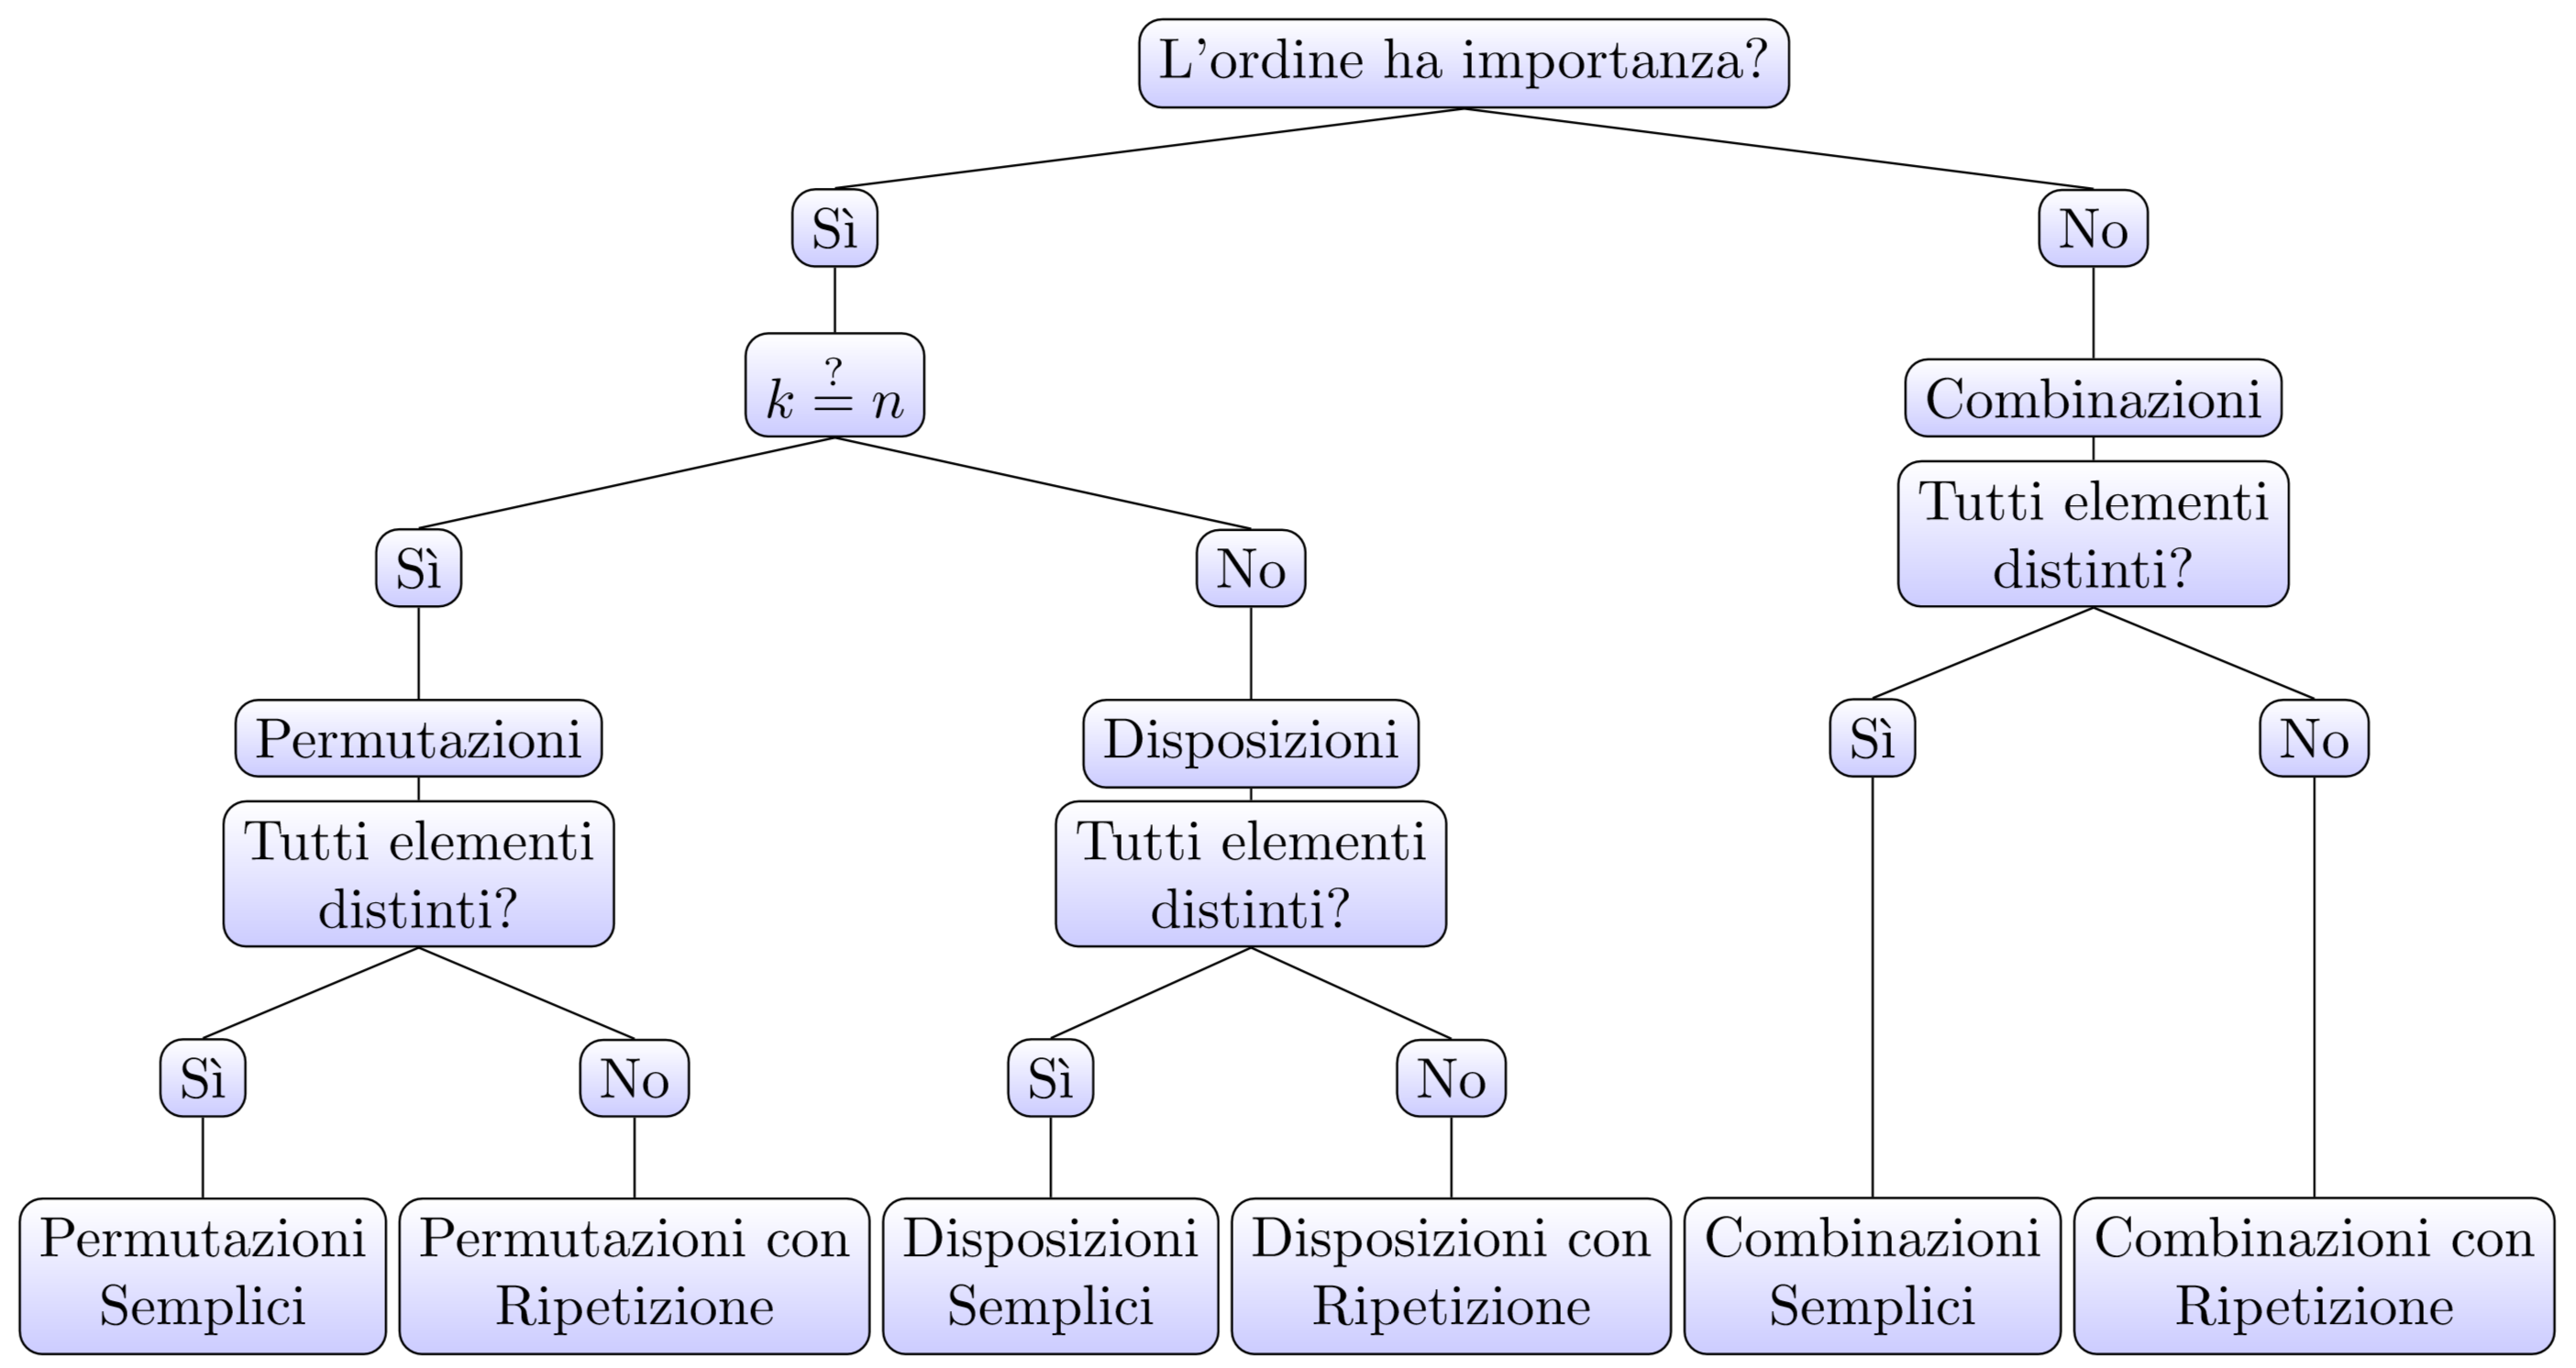
\includegraphics[width=8cm]{image/tree}
	\caption{Si risponda a ciascuna domanda per sapere che tipo di situazione il problema pone.}
\end{figure}

%!TEX ROOT=formularioMatematica.tex

\section{Probabilit�}\label{sec:prob}
La probabilit� � una funzione $p(U)$ che ritorna un valore compreso tra $0$ e $1$ che definisce la 
probilit� di un \emph{evento}.
\begin{equation*}
p:\,p(U) = \frac{\text{Casi favorevoli}}{\text{Casi possibili}}\mapsto {[{0},{1}]}
\end{equation*}

\subsection{Evento ed insieme universo}
Per un qualsiasi caso di studio esiste un insieme \emph{Universo} definito $\mathbb{U}$ che contiene
tutte le possibili uscite dell'oservazione. Ciascuna di queste uscite � definito \emph{evento}.
Quindi
\begin{equation*}
\mathbb{E} \subseteq \mathbb{U}
\end{equation*}
e detto in altri termini, un evento � un insieme di possibilit�. Ad esempio
\begin{equation*}
\mathbb{E} = \{2,4,5\}
\end{equation*}
pu� essere un evento nel lancio di un dado.\\
$p(\mathbb{U}) = 1$ per qualsiasi tipo di osservazione. Quindi la probabilit� che \textbf{non} avvenga
un evento � $1-p(\mathbb{E})$

\subsubsection{Eventi incompatibili}
Due eventi si dicono incompatibili quando
\begin{equation*}
\mathbb{E}_1 \cap \mathbb{E}_2 = \emptyset
\end{equation*}

\subsubsection{Eventi indipendenti}
Due eventi si dicono indipendenti quando
\begin{equation*}
p\left(\mathbb{E}_1\mid\mathbb{E}_2\right) = p(\mathbb{E}_1)
\end{equation*}

\subsection{Probabilit� di eventi incompatibili}
\begin{equation*}
p(\mathbb{E}_1\cup\mathbb{E}_2) = p(\mathbb{E}_1) + p(\mathbb{E}_2)
\end{equation*}

\subsection{Probabilit� di eventi compatibili}
\begin{equation*}
p(\mathbb{E}_1\cup\mathbb{E}_2) = p(\mathbb{E}_1)+p(\mathbb{E}_2)-p(\mathbb{E}_1\cap\mathbb{E}_2)
\end{equation*}
Si estenda questa formula in modo che si tolgano tutte le intersezioni fra eventi per non ripetere 
risultati.

\subsection{Probabilit� condizionata}
La probabilit� condizionata indica la probabilit� che si verifichi l'evento $\mathbb{E}_1$ 
verificatosi $\mathbb{E}_2$.
\begin{equation*}
p\left(\mathbb{E}_1\mid\mathbb{E}_2\right) = 
\frac{p\left(\mathbb{E}_1\cap\mathbb{E}_2\right)}{p(\mathbb{E}_2)}
\end{equation*}

\subsection{Probabilit� composta}
Indica la probabilit� che si verifichi un evento intersezione di altri due.
\begin{equation*}
p\left(\mathbb{E}_1\cap\mathbb{E}_2\right) = p(\mathbb{E}_1)\cdot
p\left(\mathbb{E}_1\mid\mathbb{E}_2\right)
\end{equation*}

Per� se sono eventi indipendenti si semplifica in
\begin{equation*}
p\left(\mathbb{E}_1\cap\mathbb{E}_2\right) = p(\mathbb{E}_1)\cdot p(\mathbb{E}_2)
\end{equation*}

\subsubsection{Formule di Bayes}
\subsubsection{Prima formula}
Essendo $\mathbb{F}_1, \mathbb{F}_2,\dotsc,\mathbb{F}_n$ $n$ eventi incompatibili tali che
\begin{equation*}
\mathbb{U} = \mathbb{F}_1\cup\mathbb{F}_2\cup\dotsb\cup\mathbb{F}_n
\end{equation*}
si consideri un evento $\mathbb{E}$ tale che
\begin{equation*}
\mathbb{E} = \left(\mathbb{E}\cap\mathbb{F}_1\right)\cup\left(\mathbb{E}\cap\mathbb{F}_2\right)\cup
\dots\cup\left(\mathbb{E}\cap\mathbb{F}_n\right)
\end{equation*}
si ha
\begin{equation*}
p(\mathbb{E}) = \sum\limits_{i=1}^{n}p\left(\mathbb{E}\cap\mathbb{F}_i\right) =
\sum\limits_{i=1}^{n}\big(p\left(\mathbb{E}\mid\mathbb{F}_i\right)\cdot 
p\left(\mathbb{F}i\right)\big)
\end{equation*}

\subsubsection{Seconda formula}
Essendo $\mathbb{F}_1, \mathbb{F}_2,\dotsc,\mathbb{F}_n$ $n$ eventi incompatibili tali che
\begin{equation*}
\mathbb{U} = \mathbb{F}_1\cup\mathbb{F}_2\cup\dotsb\cup\mathbb{F}_n
\end{equation*}
sia $\mathbb{E}$ un evento tale che $p(\mathbb{E})>0$, per calcolare le probabilit� condizionali si
usi
\begin{equation*}
p\left(\mathbb{F}_i\mid\mathbb{E}\right) =
\frac{p\left(\mathbb{E}\mid\mathbb{F}_i\right)\cdot p(\mathbb{F}_i)}
{\sum\big(p\left(\mathbb{E}\mid\mathbb{F}_i\right)\cdot p(\mathbb{F}_i)\big)}
\end{equation*}

%!TEX ROOT=formularioMatematica.tex

\section{Affinit�}\label{sec:aff}
Si definisce un'affinit� come una corrispondenza biunivoca tra due piani e tra punti dello stesso 
piano che trasformi rette in rette conservando il parallelismo.\\
Un'affinit� generica denominata $T$ pu� essere espressa nei seguenti modi
\begin{equation*}
T:\,\begin{cases}
x'=ax+by+e\\
y'=cx+dy+f
\end{cases}
\end{equation*}
\begin{equation*}
T:\,\begin{bmatrix}[1]
x'\\y'
\end{bmatrix}=
\begin{bmatrix}[1]
a&b\\
c&d
\end{bmatrix}
\begin{bmatrix}[1]
x\\y
\end{bmatrix}
+\begin{bmatrix}[1]
e\\f
\end{bmatrix}
\end{equation*}
\begin{equation*}
T:\,(x,y)\mapsto(ax+by+e,cx+dy+f)
\end{equation*}
Tutte le affinit� hanno il determinante della matrice dei coefficienti � sempre diverso da zero
\begin{equation*}
\begin{vmatrix}[1]
a&b\\
c&d
\end{vmatrix} = ad-cb \neq0
\end{equation*}
Se il determinante � pari a $1$ � un'isometria e quindi mantiene le distanze.\\\\

Si definisce punto unito qualunque punto che si trasforma in s� stesso, ovvero
\begin{equation*}
T(U) \equiv U (\equiv U')
\end{equation*}

Essendo le affinit� propriet� binuivoche, esiste anche la trasformazione inversa, generalmente 
indicata con $T^{-1}$.\\
Per gli esercizi si vada \hyperref[ex:aff]{qui}.

\subsection{Prodotto di trasformazioni}
Se si hanno due trasformazioni $T$ e $T'$, il loro prodotto � descritto come $T\ast T'$ e si ottiene
effettuando prima $T'$ e successivamente $T$. Quindi � equivalente a $T(T'(P))$.\\
La matrice dei coefficienti si ottiene moltiplicando le due matrici $A\ast A'$.

\subsection{Traslazione}
\begin{center}
	\begin{tikzpicture}
		\coordinate (A) at (1,2);
		\coordinate (B) at (4,3);
		
		\tkzInit[xmin=-1,ymin=-1,xmax=5,ymax=5]
		\tkzGrid
		\tkzAxeXY
		
		\filldraw (A) circle (0.05);
		\filldraw (B) circle (0.05);
		\draw[red, thick, -stealth] (A) -- (B)
			node[pos=0.5, fill=white, text=red]{$\vec{v}(a,b)$};
	\end{tikzpicture}
\end{center}
\begin{equation*}
\tau_{\begin{bmatrix}[0.7]
	\mathcolor{red}{a}\\\mathcolor{red}{b}
	\end{bmatrix}}:
\begin{cases}
x'= x+\mathcolor{red}{a}\\
y'= y+\mathcolor{red}{b}
\end{cases}
\end{equation*}
\begin{equation*}
\tau_{\begin{bmatrix}[0.7]
	\mathcolor{red}{a}\\\mathcolor{red}{b}
	\end{bmatrix}}^{-1}:
\begin{cases}
x = x'-\mathcolor{red}{a}\\
y = y'-\mathcolor{red}{b}
\end{cases}
\end{equation*}

\subsection{Rotazione}
\begin{center}
	\begin{tikzpicture}
		\coordinate (A) at (1,2);
		\coordinate (B) at (2.23,0);
		\coordinate (O) at (0,0);
		
		\tkzInit[xmin=-1,ymin=-1,xmax=5,ymax=5]
		\tkzGrid
		\tkzAxeXY
		
		\filldraw (A) circle (0.05);
		\filldraw (B) circle (0.05);
		\path[thick, red, -stealth, bend left] (A) edge (B);
		\draw (O) -- (A);
		\markangle{O}{A}{B}{0.5}{1.5}{$\theta$}
	\end{tikzpicture}
\end{center}
\begin{equation*}
\rho_{O,\theta}:\,\begin{cases}
x'=x\cos\theta-y\sin\theta\\
y'=x\sin\theta+y\cos\theta
\end{cases}
\end{equation*}
\begin{equation*}
\rho_{O,\theta}:\,\begin{cases}
x=x'\cos\theta+y'\sin\theta\\
y=-y'\sin\theta+y\cos\theta
\end{cases}
\end{equation*}

\subsection{Simmetria centrale}
\begin{center}
	\begin{tikzpicture}
		\coordinate (A) at (-1,0);
		\coordinate (B) at (2,0);
		\coordinate (C) at (0.5,0);
		
		\tkzInit[xmin=-1.5,ymin=-1,xmax=2.5,ymax=1]
		\tkzGrid
		\tkzAxeXY
		
		\filldraw (A) circle (0.05);
		\filldraw (B) circle (0.05);
		\filldraw (C) circle (0.05);
		\draw (A) -- (B);
		\path[thick, red, bend left, -stealth] (A) edge (B);
	\end{tikzpicture}
\end{center}

\begin{equation*}
\sigma_{C(x_C,y_C)}:\,\begin{cases}
x'= -x+2x_C\\
y'= -y+2y_C
\end{cases}
\end{equation*}
\begin{equation*}
\sigma_{C(x_C,y_C)}^{-1}:\,\begin{cases}
x = -x'+2x_C\\
y = -y'+2y_C
\end{cases}
\end{equation*}

\subsection{Simmetria assiale}
\begin{center}
	\begin{tikzpicture}
		\coordinate (A) at (-2,0);
		\coordinate (B) at (-1,1);
		\coordinate (C) at (1,1);
		\coordinate (D) at (2,0);
		
		\tkzInit[xmin=-3,ymin=-1,xmax=3,ymax=2]
		\tkzGrid
		\tkzAxeXY
		
		\filldraw (A) circle (0.05);
		\filldraw (B) circle (0.05);
		\filldraw (C) circle (0.05);
		\filldraw (D) circle (0.05);
		\draw (A) -- (B);
		\draw (C) -- (D);
		\draw[-stealth, red, thick] (-1.5,0.5) -- (1.5,.5);
	\end{tikzpicture}
\end{center}

\subsubsection{Rispetto a $r:\,y=y_0$}
\begin{equation*}
\sigma_r:\,\begin{cases}
x'= x\\
y'= -y+2y_0
\end{cases}
\end{equation*}

\subsubsection{Rispetto a $r:\,x=x_0$}
\begin{equation*}
\sigma_r:\,\begin{cases}
x'= -x+2x_0\\
y'=y
\end{cases}
\end{equation*}

\subsubsection{Rispetto a $r:\,y=mx+q$}
\begin{equation*}
\sigma_r:\,\begin{cases}
x'=\frac{1}{1+m^2}[(1-m^2)x+2my-2mq]\\
y'=\frac{1}{1+m^2}[2mx+(m^2-1)y+2q]
\end{cases}
\end{equation*}

\begin{equation*}
\sigma_r^{-1}:\,\begin{dcases}
x=\frac{1}{1+m^2}[(1-m^2)x +2my'-2mq]\\
y=\frac{1}{1+m^2}[2mx'+(m^2-1)y'+2q]
\end{dcases}
\end{equation*}

\subsection{Similitudine}
\begin{center}
	\begin{tikzpicture}[scale=0.75]
		\coordinate (A) at (-2,0);
		\coordinate (B) at (0,4);
		\coordinate (O) at (0,0);
		\coordinate (C) at (-4,6);
		\coordinate (D) at (-2,-5);
		\coordinate (E) at (2,-2);
		
		\tkzInit[xmin=-5,ymin=-6,xmax=3,ymax=7]
		\tkzGrid
		\tkzAxeXY
		
		\filldraw (A) circle (0.05);
		\filldraw (B) circle (0.05);
		\filldraw (C) circle (0.05);
		\filldraw (D) circle (0.05);
		\filldraw (E) circle (0.05);
		\filldraw (O) circle (0.05);
		
		\filldraw[thick, cyan, fill opacity = 0.3] (A) -- (B) -- (O) -- cycle;
		\filldraw[thick, red, fill opacity = 0.3] (C) -- (D) -- (E) -- cycle;
		\path[-stealth, red, thick, bend left] (-0.5,2) edge (0.7,-1);
	\end{tikzpicture}
\end{center}

\begin{equation*}
\Sigma:\,
\begin{cases}
\begin{cases}
x'= ax-by+e\\
y'= bx+ay+f
\end{cases}\text{Se diretta, }\det A = \begin{vmatrix}[1]
a&-b\\b&-a
\end{vmatrix}>0\\
\begin{cases}
x'=ax+by+e\\
y'=bx-ay+f
\end{cases}\text{Se indiretta, }\det A = \begin{vmatrix}[1]
a&b\\b&-a
\end{vmatrix}<0
\end{cases}
\end{equation*}
Il rapporto di similitudine � pari a 
\begin{equation*}
k = \sqrt{a^2+b^2}
\end{equation*}

\subsection{Omotetia}
\begin{center}
	\begin{tikzpicture}[scale=0.5]
		\coordinate (A) at (-2,0);
		\coordinate (B) at (-1,1);
		\coordinate (O) at (0,0);
		\coordinate (C) at (-3,-2);
		\coordinate (D) at (4,0);
		\coordinate (E) at (2,-2);
		\coordinate (F) at (6,4);
		
		\tkzInit[xmin=-4,ymin=-3,xmax=7,ymax=5]
		\tkzGrid
		\tkzAxeXY
		
		\filldraw (A) circle (0.05);
		\filldraw (B) circle (0.05);
		\filldraw (C) circle (0.05);
		\filldraw (D) circle (0.05);
		\filldraw (E) circle (0.05);
		\filldraw (F) circle (0.05);
		\filldraw (O) circle (0.05);
		
		\filldraw[thick, cyan, fill opacity = 0.3] (A) -- (B) -- (C) -- cycle;
		\filldraw[thick, red, fill opacity = 0.3] (D) -- (E) -- (F) -- cycle;
		\path[-stealth, red, thick, bend left] (-1,-0.5) edge (3.5,1);
		\draw[dashed] (A) -- (D);
		\draw[dashed] (B) -- (E);
		\draw[dashed] (C) -- (F);
	\end{tikzpicture}
\end{center}

\begin{equation*}
\omega_{C,a}:\,\begin{cases}
x'=a(x-x_C)+x_C\\
y'=a(y-y_C)+y_C
\end{cases} \rightarrow
\begin{cases}
x'= ax+h\\
y'= ay+k
\end{cases}
\end{equation*}

\subsection{Dilatazione}
\begin{center}
	\begin{tikzpicture}
		\tkzInit[xmin=-1,ymin=-1,xmax=4,ymax=3]
		\tkzGrid
		\tkzAxeXY
		\filldraw[thick, cyan, fill opacity = 0.3] (0,0) -- (2,0) -- (2,2) -- (0,2) -- cycle;
		\filldraw[thick, red, fill opacity = 0.3] (2,2) -- (3,2) -- (3,0) -- (2,0);
		\path[-stealth, thick, red] (1,1) edge (2.5,1);
	\end{tikzpicture}
\end{center}

\begin{equation*}
\delta_{x,k}:\,\begin{cases}
x'=kx\\
y'=y
\end{cases}\quad\delta_{y,k}:\,\begin{cases}
x'=x\\
y'=ky
\end{cases}
\end{equation*}

\subsection{Inclinazione}
\begin{center}
	\begin{tikzpicture}
		\tkzInit[xmin=-1,ymin=-1,xmax=6,ymax=3]
		\tkzGrid
		\tkzAxeXY
		\filldraw[thick, cyan, fill opacity = 0.3] (0,0) -- (2,0) -- (2,2) -- (0,2) -- cycle;
		\filldraw[thick, red, fill opacity = 0.3] (0,0) -- (2,0) -- (5,2) -- (3,2) -- cycle;
		\path[-stealth, thick, red] (1,1) edge (2.5,1);
	\end{tikzpicture}
\end{center}
\begin{equation*}
\xi_{x,k}:\,\begin{cases}
x'=x_ky\\
y'=y
\end{cases}\quad\xi_{y,k}:\,\begin{cases}
x'=x\\
y'=y+kx
\end{cases}
\end{equation*}

%!TEX ROOT=formularioMatematica.tex

\section{Numeri complessi}\label{sec:complex}
Fino ad adesso abbiamo sempre lavorato con numeri appartenenti ad $\mathbb{R}$ al di pi�. Ci sono per�
alcune operazioni che non sono possibili da fare in questo insieme numerico. Una di queste �
\begin{equation*}
\sqrt{-r}\qquad\forall r\in\mathbb{R}^+
\end{equation*}
oppure
\begin{equation*}
\log(n)\qquad \forall n\in\mathbb{R}^-
\end{equation*}
Per sopperire a questa mancanza, � stata introdotta l'unit� immaginaria $i$ che � definita come
\begin{equation*}
i=\sqrt{-1}
\end{equation*}
Un numero complesso � un numero composto da una parte reale e una immaginaria. Esso pu� essere scritto
come
\begin{equation*}
z = \overbrace{a}^{\text{Reale}} + \overbrace{ib}^{\text{Immaginaria}}
\end{equation*}
Quindi
\begin{equation*}
\Re(z) = a \quad\text{e}\quad\Im(z)=ib
\end{equation*}
Questo non � l'unico modo di identificare un numero complesso. Pi� avanti vedremo anche gli altri.\\
$\mathbb{C}$ � quindi definito come
\begin{equation*}
\mathbb{C}=\left\{a+ib: a,b\in\mathbb{R}\right\}
\end{equation*}
Il numero complesso $\bar{z}$ � definito il \textit{coniugato} di $z$ quindi
\begin{equation*}
z=a+ib\qquad\text{e}\qquad\bar{z}=a-ib
\end{equation*}
Si noti che se si deve fare ricorso a \hyperref[ruffini]{Ruffini} si ricerchi lo zero anche in 
$\mathbb{C}$.\\
Per gli esercizi si vada \hyperref[ex:complex]{qui}.

\subsection{Rappresentazione cartesiana}\label{subsec:complex:cart}
Essendo questo numero composto da parte reale e immaginaria, il piano cartesiano non basta pi�. Quindi 
si � deciso di estenderlo a quello che viene comunemente denominato il piano di \textbf{Argrand-Gauss}.
Esso � composto dall'asse delle ascisse come parte reale e quello delle ordinate come parte 
immaginaria.

\begin{center}
	\begin{tikzpicture}
		\coordinate (A) at (1,1.5);
		\coordinate (O) at (0,0);
		\coordinate (B) at (2,0);
		
		\tkzInit[xmin=-2,ymin=-2,xmax=2,ymax=2]
		\tkzGrid
		\tkzAxeXY
		\filldraw[red] (A) circle (0.05);
		\draw[-stealth] (O) -- (A);
		\markangle{O}{A}{B}{0.5}{1.5}{$\theta$}
		\node[above right] at (A) {$P(a,b)$};
	\end{tikzpicture}
\end{center}

La distanza $\overline{OP}$ � detta \emph{modulo} del numero immaginario ed � descritto come
\begin{equation*}
\rho=\norm{z} = \sqrt{a^2+b^2}
\end{equation*}

\subsection{Operazioni tra numeri complessi}
\subsubsection{Somma}
La somma tra due numeri complessi richiede solo di sommare le parti simili fra di loro.
\begin{align*}
&z_1=a_1+i+b_1\qquad\text{e}\qquad z_2=a_2+i_b2
\intertext{La loro somma �}
&z=z_1+z_2=a_1+a_2+i(b_1+b_2)
\end{align*}
Nella somma vige la seguente caratteristica
\begin{equation*}
\overline{z_1+z_2} = \overline{z_1}+\overline{z_2}
\end{equation*}

\subsubsection{Differenza}
La differenza � esattamente come la somma, ovvero si opera parte a parte.
\begin{align*}
&z_1=a_1+i+b_1\qquad\text{e}\qquad z_2=a_2+i_b2
\intertext{La loro differenza �}
&z=z_1-z_2=a_1-a_2+i(b_1-b_2)
\end{align*}
Nella somma e differenza vigono le seguenti caratteristiche
\begin{equation*}
z+\overline{z}=2a\qquad\text{e}\qquad z-\overline{z}=2ib
\end{equation*}

\subsubsection{Prodotto}
Il prodotto si effettua moltiplicando fra di loro parti simili.
\begin{align*}
&z_1=a_1+i+b_1\qquad\text{e}\qquad z_2=a_2+i_b2
\intertext{Il loro prodotto �}
&z=z_1\cdot z_2=a_1a_2-b_1b_2+i(b_1a_2+a_1b_2)
\end{align*}	

\subsubsection{Quoziente}
Il quoziente � un'operazione particolare.
\begin{align*}
&z_1=a_1+i+b_1\qquad\text{e}\qquad z_2=a_2+i_b2
\intertext{Il loro quoziente �}
&z=\frac{z_1}{z_2}=\frac{a_1a_2+b_1b_2}{a_2^2+b_2^2}+i\frac{b_1a_2-a_2b_2}{a_2^2+b_2^2}
\end{align*}

\subsection{Rappresentazione trigonometrica di un numero complesso}
Un modo per definire un numero complesso � gi� stato chiarito. Ne esiste un altro per� che fa capo
alla rappresentazione polare del numero (tramite un altro sistema di assi che identifica un punto
tramite l'angolo che compie un segmento dall'asse $x$).
\begin{equation*}
z=\rho(\cos\theta+i\sin\theta)
\end{equation*}
dove $\theta$ rappresenta l'angolo indicato nella sottosezione
\hyperref[subsec:complex:cart]{Rappresentazione cartesiana}.

\subsubsection{Prodotto}
\begin{align*}
&z_1=\rho_1(\cos\theta_1+i\sin\theta_1)\quad\text{e}\quad z_2=\rho_2(\cos\theta_2+i\sin\theta_2)
\intertext{Il loro prodotto �}
&z=z_1\cdot z_2=\rho_1\rho_2[\cos(\theta_1+\theta_2)_i\sin(\theta_1+\theta_2)]
\end{align*}
\subsubsection{Quoziente}
\begin{align*}
&z_1=\rho_1(\cos\theta_1+i\sin\theta_1)\quad\text{e}\quad z_2=\rho_2(\cos\theta_2+i\sin\theta_2)
\intertext{Il loro quoziente �}
&z=\frac{z_1}{z_2}=\frac{\rho_1}{\rho_2}[\cos(\theta_1-\theta_2)_i\sin(\theta_1-\theta_2)]
\end{align*}

\subsection{Elevazione a potenza}
Messa successivamente alle altre operazioni perch� varia in base alla notazione scelta.
\subsubsection{Algebrica}
\begin{equation*}
z^n = (a+ib)^n
\end{equation*}
\subsubsection{Trigonometrica (Formula di De Moivre)}
\begin{equation*}
z^n=\rho^n(\cos n\theta+i\sin n\theta)
\end{equation*}

\subsection{Radici di un numero complesso}
\begin{align*}
&z = \rho(\cos\theta+i\sin\theta)
\intertext{La radice $n$-esima � pari a}
&\sqrt[n]{z}=\sqrt[n]{\rho}\left(\cos\frac{\theta+2k\pi}{n}+i\sin\frac{\theta+2k\pi}{n}\right)
\end{align*}
Una caratteristica interessante delle radici � la loro rappresentazione grafica. Infatti se si prendono
le coordinate e si uniscono fra di loro si costruir� un poligono regolare con $n$ lati inscritto 
all'interno di una circonferenza di raggio $\rho$.\\
Per calcolarle, sostituire $k$ con i numeri che vanno da $0$ a $n-1$.

\subsection{Teroema fondamentale dell'algebra}
Esso cita:
\begin{tfa}
	Ogni polinomio di grado $n\geq1$
	\begin{equation*}
	P(x) = \sum\limits_{i=0}^{n} a_ix^i
	\end{equation*}
	a coefficienti $\mathbb{C}$ ha almeno uno zero in $\mathbb{C}$.
\end{tfa}
Da questo deriva
\begin{tfa-ext}
	Per ogni polinomio di grado $n\geq1$
	\begin{equation*}
	P(x) = \sum\limits_{i=0}^{n} a_ix^i
	\end{equation*}
	a coefficienti $\mathbb{C}$ ha esattamente $n$ zeri in $\mathbb{C}$, con la convenzione di contare
	$r$ volte uno zero di molteplicit� $r$.
\end{tfa-ext}
Per molteplicit� si intende
\begin{molteplic}
	Se il polinomio $P(x)$ si pu� scomporre nel prodotto
	\begin{equation*}
	P(x) = (x-\alpha)^rP_r(x)
	\end{equation*}
	dove il polinomio $P_r(x)$ � di grado $(n-r)$, si dice che $P(x)$ � divisibile per $(x-\alpha)^r$
	e se $P_r(x)$ non � divisibile per $(x-\alpha)$, si dice che $\alpha$ � uno \textbf{zero di 
	molteplicit�} $r$ per $P(x)$.
\end{molteplic}

\subsection{Esponenziali complessi}
Detta $e$ la costante di Nepero (anche chiamato numero di Eulero)
\begin{equation*}
e \approx 2.71828\ldots
\end{equation*}
si definisce per ogni numero complesso $z = a+ib$ l'esponenziale complesso $e^{a+ib}$ come il numero
complesso 
\begin{equation*}
w=e^x(\cos a+i\sin b)
\end{equation*}
Quindi possiamo dire che 
\begin{equation*}
e^{z} = \rho e^{i\theta}
\end{equation*}
Proprio da questa formula ne viene ricavata una delle pi� famose della storia della matematica
\begin{equation*}
e^{i\pi}+1=0
\end{equation*}
che collega 5 unit� fondamentali della matematica.

\subsection{Formule di Eulero}
\begin{equation*}
\cos\theta=\frac{e^{i\theta}+e^{-i\theta}}{2}\qquad\sin\theta=\frac{e^{i\theta}-e^{-i\theta}}{2}
\end{equation*}
Queste formule permettono di trasferire tutte le caratteristiche della notazione trigonometrica in 
quella esponenziale.
%!TEX ROOT=formularioMatematica.tex

\section{Insiemi numerici}\label{sec:insiemi}
Se durante la nostra carriera scolastica abbiamo sempre lavorato con $\mathbb{R}$ o al massimo in 
$\mathbb{C}$, nulla vieta che noi creiamo nuovi insiemi numerici e li studiamo per trovarne alcune
caratteristiche.\\
Ogni insieme numerico possiede delle caratteristiche che noi possiamo studiare
\begin{enumerate}
	\item È limitato/illimitato
	\item Possiede un $\max$ e un $\min$
	\item Possiede \emph{maggioranti} o \emph{minoranti}
	\item Possiede un $\sup$ o un $\inf$
\end{enumerate}
Per le seguenti definizioni ed esempi, prenderemo in considerazione
\begin{equation*}
A = \left\{\frac{1}{n}\mid n\in\mathbb{N}_0\right\}
\end{equation*}

\subsection{Condizioni di limitazione}
La o le condizioni di limitazione indicani quale può essere un limite o i limiti di un insieme. In 
insieme può essere illimitato (ovvero che per qualunque numero noi scegliamo, esisterà un punto
sulla retta che lo rappresenta), limitato \emph{superiormente}, \emph{inferiormente} o entrambi
contemporaneamente.\\
In generale la condizione di limitazione (superiore ed inferiore per uno stesso valore) è
\begin{equation*}
\exists\,k>0\land k\in\mathbb{R}\mid \forall x \in A, \abs{x} \leq k
\end{equation*}
Generalizzando ancora per due valori diversi
\begin{equation*}
\exists\,k_1,k_2>0\land k_1,k_2\in\mathbb{R}\mid \forall x\in A, k_1\leq x \leq k_2
\end{equation*}

\subsection{Maggioranti e minoranti}
Prendendo le condizioni di limitazione separatamente
\begin{align*}
\exists\,m\in\mathbb{R}\mid\forall x\in A x\geq m
\intertext{e}
\exists\,M\in\mathbb{R}\mid\forall x\in A x\leq M
\end{align*}
$m$ rappresenta un \textbf{minorante} di $A$ e $M$ rappresenta un \textbf{maggiorante} di $A$.

\subsection{Massimi e minimi}
Un numero si definisce \emph{massimo} se
\begin{equation*}
\exists\,L\in\mathbb{A}\mid\forall x\in A, L\geq x
\end{equation*}
quindi è il valore più alto che l'insieme contiene.\\
Un numero si definisce \emph{minimo} se
\begin{equation*}
\exists\,l\in\mathbb{A}\mid\forall x\in A, l\leq x
\end{equation*}
quindi è il valore più basso che l'insieme contiene.

\subsection{Intervalli}
Un \emph{intervallo} può essere aperto (illimitato) o chiuso (limitato). La notazione più comune è la 
seguente
\begin{align*}
\textbf{Limitato }&{[{1},{4}]}\coloneqq\{x\in\mathbb{R}\mid1\leq x \leq4\}\\
\textbf{Illimitato }&{]{-\infty},{\pi}[}\coloneq\{x\in\mathbb{R}\mid-\infty<x<\pi\}
\end{align*}
Da notare che $\pm\infty$ è sempre escluso in quanto tecnicamente non appartiene a $\mathbb{R}$.\\
Un \emph{intorno} non è altro che un intervallo che comprende un numero specifico. In simboli
\begin{equation*}
I(x_0)\coloneqq{]{x_0-\delta_1},{x_0+\delta_2}[} \qquad(\delta_1,\delta_2\in\mathbb{R})
\end{equation*}
Ovviamente si può definire un intorno che sia limitato con una distanza
\begin{equation*}
I_\varepsilon(x_0)\coloneqq{]{x_0-\varepsilon},{x_0+\varepsilon}[} 
\end{equation*}
Questo è completo e ovviamente possiamo anche fare intorni non completi (quindi solo da un lato). Essi 
sono di conseguenza denominati sinistri o destri.

\subsection{Punti isolati}
Un punto isolato è un punto i cui intorni non contengono alcun elemento dell'insieme.
\begin{equation*}
x_0\in A, \exists\,I(x_0)\mid\forall x\in A\setminus\{x_0\}\not\supset I(x_0)
\end{equation*}

\subsection{Punti di accumulazione}
Un punto di accumulazione è un punto in cui ogni suo intorno cade almeno un elemento distinto 
dell'insieme.
\begin{equation*}
x_0,y\in A,\forall I(x_0), y\in I(x_0)
\end{equation*}

\subsection{Estremi}
L'estremo superiore è quel valore che non viene mai superato. A seconda dei casi può essere il 
\emph{più grande elemento dell'insieme} o il \emph{più piccolo dei maggioranti}.
\begin{equation*}
\forall x\in A\implies x\leq\Lambda\quad\text{e}\quad \forall\varepsilon\in\mathbb{R}_0^+,
\exists\,x\in A\mid x>\Lambda-\varepsilon
\end{equation*}
L'estremo inferiore è quel valore che non non ha valori inferiori. A seconda dei casi può essere il
\emph{più piccolo elemento dell'insieme} o il \emph{più grande dei minoranti}.
\begin{equation*}
\forall x\in A\implies x\geq\lambda\quad\text{e}\quad \forall\varepsilon\in\mathbb{R}_0^+,
\exists\,x\in A\mid x<\lambda+\varepsilon
\end{equation*}
%!TEX ROOT=formularioMatematica.tex

\section{Limiti}\label{sec:limiti}
Per introdurre il concetto di limite, prendiamo ad esempio la funzione
\begin{equation*}
  f:\,\mathscr{D}_f\mapsto\mathbb{R}\mid x\mapsto\frac{2x^2-8}{x-2}
\end{equation*}
essendo
\begin{equation*}
  \mathscr{D}_f=\mathbb{R}-\{2\}
\end{equation*}
La funzione non è definita per $x = 2$ però possiamo comunque trovare i valori della funzione per numeri
che si avvicinano sempre più a $2$
\begin{center}
  \begin{tabular}{cc}
    $\boldsymbol{x}$ & $\boldsymbol{f(x)}$\\\hline
    $1$ & $6$\\
    $1.5$ & $7$\\
    $1.9$ & $7.8$\\
    $1.9991$ & $7.9982$\\
    $\ldots$ & $\ldots$\\
    $2.0001$ & $8.002$\\
    $2.1$ & $8.2$\\
    $2.5$ & $9$\\
    $3$ & $10$ 
  \end{tabular}
\end{center}
Come notiamo dalla tabella, più i ci si avvicina a $2$ più i valori si avvicinano a $8$. A questo
comportamento diamo il nome di \textbf{limite finito}.\\
Possiamo quindi dire che per un numero $\varepsilon$ positivo
\begin{equation*}
  \left\lvert\frac{2x^2-8}{x-2}-8\right\rvert<\varepsilon
\end{equation*}
Questa disequazione ammette come soluzioni un intervalo opportuno di centro $x=2$. Tenuto conto che
\begin{align*}
  &2x^2-8=2(x-2)(x+2)
  \intertext{riducendo}
  &\abs{2x-4}<\varepsilon\quad x \neq 2
  \intertext{ovvero}
  &-\varepsilon<2x-4<\varepsilon\quad x \neq 2
  \intertext{ossia}
  &2-\frac{\varepsilon}{2}<x<2+\frac{\varepsilon}{2}\quad x \neq 2
  \intertext{Questo vuol dire che se}
  &x\in{\left]{2-\frac{\varepsilon}{2}},{2+\frac{\varepsilon}{2}}\right[}\quad x \neq 2
  \intertext{i corrispondenti valori di $f(x)$ distano da $8$ meno di $\varepsilon$}
\end{align*}
Scriveremo allora
\begin{equation*}
  \lim\limits_{x\to2}\frac{2x^2-8}{x-2}=8
\end{equation*}
che si legge \emph{il limite per $x$ che tende a $2$ di $\frac{2x^2-8}{x-2}$ è uguale a $8$}.\\\\
Consideriamo ora la funzione
\begin{equation*}
  f:\,\mathscr{D}_f\mapsto\mathbb{R}\mid x\mapsto\frac{1}{(x+1)^2}
\end{equation*}
essendo
\begin{equation*}
  \mathscr{D}_f = \mathbb{R}-\{-1\}
\end{equation*}
Attribuiamo ora a $x$ valori sempre più vicini a $-1$
\begin{center}
  \begin{tabular}{cc}
    $\boldsymbol{x}$ & $\boldsymbol{f(x)}$\\\hline
    $-2$ & $1$\\
    $-1.5$ & $4$\\
    $-1.001$ & $1,000,000$\\
    $\ldots$ & $\ldots$\\
    $0$ & $1$\\
    $-0.5$ & $4$\\
    $-0.99995$ & $400,000,000$
  \end{tabular}
\end{center}
Notiamo che per valori che si avvicinano a $-1$ otteniamo sempre valori molto grandi. A questo 
comportamento si da il nome di \textbf{limite a più infinito ($+\infty$)}.\\
Quindi si può scrivere
\begin{equation*}
  \lim\limits_{x\to-1}\frac{1}{(x+1)^2}=+\infty
\end{equation*}
che sgnifica che comunque si prenda un numero $M$ la disuguaglianza
\begin{equation*}
  \frac{1}{(x+1)^2}>M
\end{equation*}
è soddisfatta dai punti di un intorno di $-1$, escluso $-1$ stesso.\\
Supposto che $x\neq-1$ l'equazione equivale a
\begin{align*}
  &(x+1)^2<\frac{1}{M}
  \intertext{verificata per}
  &-\frac{1}{\sqrt{M}}<x+1<\frac{1}{\sqrt{M}}
  \intertext{cioè}
  &-1-\frac{1}{\sqrt{M}}<x<-1+\frac{1}{\sqrt{M}}\quad x\neq-1
\end{align*}
Tali valori effettivamente rappresentano un intorno di $-1$ escluso $-1$ stesso.\\
Analogamente al limite che tende a $+\infty$, si può trovare il limite a $-\infty$.\\\\
Un problema simile a quelli precedenti è quello di un valore che dopo un po' si stabilizza. In altre
parole, un valore che tendendo ad $\infty$ tende ad un numero finito. Questi sono definiti \textbf{
limiti finiti di una funzione all'infinito}. In simboli
\begin{equation*}
  \lim\limits_{x\to+\infty}f(x)=l
\end{equation*}
Possiamo ulteriormente estendere il concetto a \textbf{limiti infiniti di una funzione all'infinito}.
Ad esempio
\begin{equation*}
  \lim\limits_{x\to-\infty}f(x)=+\infty
\end{equation*}


\subsection{Definizione di limite finito}
\begin{definizioneLimiteFinito}
  Sia $f$ una funzione definita in un intorno $I$ del punto $x_0$, senza che sia necessariamente
  definita in $x_0$.\\
  Si dice che il numero $l$ è il \textbf{limite} della funzione $f$ nel punto $x_0$ e si scrive
  \begin{equation*}
    \lim\limits_{x\to x_0}f(x)=l
  \end{equation*}
  se, fissato comunque un numero $\varepsilon>0$, è possibile determinare in corrispondenza di esso 
  un numero $\delta_\varepsilon>0$ tale che, per ogni $x$ appartenente a $I$ verificante la 
  condizione
  \begin{equation*}
    0<\abs{x-x_0}<\delta_\varepsilon
  \end{equation*}
  risulti
  \begin{equation*}
    \abs{f(x)-l}<\varepsilon
  \end{equation*}
  In simboli
  \begin{align*}
    \lim\limits_{x\to x_0} f(x) &= l\\
    \ArrowBetweenLines
    \forall \varepsilon, \exists\,\delta_\varepsilon>0\mid\forall x: 0<\vert x-x_0\vert 
    &<\delta_\varepsilon \Rightarrow \vert f(x) - l\vert < \varepsilon
  \end{align*}
\end{definizioneLimiteFinito}

\subsection{Definizione di limite infinito}
\subsubsection{A $+\infty$}
\begin{definizioneLimiteInfinito1}
  Sia $f$ una funzione definita in un intorno $I$ di $x_0$, escluso al più il punto $x_0$. Si dice
  che
  \begin{equation*}
    \lim\limits_{x\to x_0}f(x)=+\infty
  \end{equation*}
  se, fissato comunque un numero $M$, è possibile determinare in corrispondenza di esso un numero
  $\delta_M>0$ tale che, per ogni $x$ di $I$ verificante la condizione
  \begin{equation*}
    0<\abs{x-x_0}<\delta_M
  \end{equation*}
  risulti
  \begin{equation*}
    f(x)>M
  \end{equation*}
  In simboli
  \begin{align*}
    \lim\limits_{x\to x_0} f(x) &= l\\
    \ArrowBetweenLines
    \forall M>0, \exists\,\delta_M>0\mid\forall x: 0<\vert x-&x_0\vert < \delta_M \Rightarrow
    f(x) > M
  \end{align*}
\end{definizioneLimiteInfinito1}
\subsubsection{A $-\infty$}
\begin{definizioneLimiteInfinito2}
  Sia $f$ una funzione definita in un intorno $I$ di $x_0$, escluso al più il punto $x_0$. Si dice
  che
  \begin{equation*}
    \lim\limits_{x\to x_0}f(x)=-\infty
  \end{equation*}
  se, fissato comunque un numero $M$, è possibile determinare in corrispondenza di esso un numero
  $\delta_M>0$ tale che, per ogni $x$ di $I$ verificante la condizione
  \begin{equation*}
    0<\abs{x-x_0}<\delta_M
  \end{equation*}
  risulti
  \begin{equation*}
    f(x)<M
  \end{equation*}
  In simboli
  \begin{align*}
    \lim\limits_{x\to x_0} f(x) &= l\\
    \ArrowBetweenLines
    \forall M, \exists\,\delta_M>0\mid\forall x: 0<\vert x-x_0\vert &< \delta_M \Rightarrow
    f(x) < M
  \end{align*}
\end{definizioneLimiteInfinito2}

\subsection{Definizione di limite finito di una funzione all'infinito}
\subsubsection{Per $x\to+\infty$}
\begin{definizioneLimiteInfinitoFinito1}
  Sia $f$ una funzione definita in un insieme $\mathscr{D}_f$ illimitato superiormente.\\
  Si dice che
  \begin{equation*}
    \lim\limits_{x\to+\infty}f(x)=l
  \end{equation*}
  se, fissato comunque un numero $\varepsilon>0$ è possibile determinare in corrispondenza di esso 
  un numero $k_\varepsilon$ tale che, per ogni $x\in\mathscr{D}_f$ e maggiore di $k_\varepsilon$, 
  risulti
  \begin{equation*}
    \abs{f(x)-l}<\varepsilon
  \end{equation*}
  In simboli
  \begin{align*}
    \lim\limits_{x\to x_0} f(x) &= l\\
    \ArrowBetweenLines
    \forall \varepsilon, \exists\,k_\varepsilon>0\mid\forall x: x>&k_\varepsilon \Rightarrow
    \vert f(x) - l\vert < \varepsilon
  \end{align*}
\end{definizioneLimiteInfinitoFinito1}
\subsubsection{Per $x\to-\infty$}
\begin{definizioneLimiteInfinitoFinito2}
  Sia $f$ una funzione definita in un insieme $\mathscr{D}_f$ illimitato superiormente.\\
  Si dice che
  \begin{equation*}
    \lim\limits_{x\to-\infty}f(x)=l
  \end{equation*}
  se, fissato comunque un numero $\varepsilon>0$ è possibile determinare in corrispondenza di esso 
  un numero $k_\varepsilon$ tale che, per ogni $x\in\mathscr{D}_f$ e minore di $k_\varepsilon$, 
  risulti
  \begin{equation*}
    \abs{f(x)-l}<\varepsilon
  \end{equation*}
  In simboli
  \begin{align*}
    \lim\limits_{x\to x_0} f(x) &= l\\
    \ArrowBetweenLines
    \forall \varepsilon, \exists\,k_\varepsilon>0\mid\forall x: x<&k_\varepsilon \Rightarrow
    \vert f(x) - l\vert < \varepsilon
  \end{align*}
\end{definizioneLimiteInfinitoFinito2}

\subsection{Definizione di limite infinito di una funzione all'infinito}
\subsubsection{A $+\infty$}
\begin{definizioneLimiteInfinitoInfinito1}
  Sia $f$ una funzione definita in un insieme $\mathscr{D}_f$ illimitato superiormente 
  [inferiormente]. Si dice che
  \begin{equation*}
    \lim\limits_{\substack{x\to+\infty\\ [x\to-\infty]}}f(x)=+\infty
  \end{equation*}
  se, fissato comunque un numero $M$, è possibile determinare in corrispondenza di esso un numero 
  $k_M$ tale che, per ogni $x\in\mathscr{D}_f$ che verifichi la condizione $x>k_M\,[x<k_M]$, risulti
  \begin{equation*}
    f(x)>M
  \end{equation*}
  In simboli
  \begin{align*}
    \lim\limits_{\substack{x\to+\infty\\ [x\to-\infty]}}f(x)&=+\infty\\
    \ArrowBetweenLines
    \forall k_M>0, \exists\,M>0\mid\forall x: x>&k_M[<k_M] \Rightarrow f(x) > M
  \end{align*}
\end{definizioneLimiteInfinitoInfinito1}
\subsubsection{A $-\infty$}
\begin{definizioneLimiteInfinitoInfinito2}
  Sia $f$ una funzione definita in un insieme $\mathscr{D}_f$ illimitato superiormente 
  [inferiormente]. Si dice che
  \begin{equation*}
    \lim\limits_{\substack{x\to+\infty\\ [x\to-\infty]}} f(x)=-\infty
  \end{equation*}
  se, fissato comunque un numero $M$, è possibile determinare in corrispondenza di esso un numero 
  $k_M$ tale che, per ogni $x\in\mathscr{D}_f$ che verifichi la condizione $x>k_M\,[x<k_M]$, risulti
  \begin{equation*}
    f(x)<M
  \end{equation*}
  In simboli
  \begin{align*}
    \lim\limits_{\substack{x\to+\infty\\ [x\to-\infty]}}f(x)&=+\infty\\
    \ArrowBetweenLines
    \forall k_M, \exists\,M>0\mid\forall x: x>k_M&[<k_M] \Rightarrow f(x) < M
  \end{align*}
\end{definizioneLimiteInfinitoInfinito2}

\subsection{Limite sinistro e destro}
Avere limite $l$ in un punto $x_0$ significa per una funzione essere regolare, ovvero assumere valori
sempre più prossimi a $l$ tanto $x$ è prossimo a $x_0$.\\
Questa regolarità però può mancare in senso assoluto. Ciò avviene quando la funzione si stabilizza
su due numeri diversi a seconda che ci si avvicini da destra o da sinistra.
\begin{equation*}
  \lim\limits_{x\to x_0^+}f(x)
\end{equation*}
indica un limite destro,
\begin{equation*}
  \lim\limits_{x\to x_0^-}f(x)
\end{equation*}
un limite sinistro.
\begin{definizioneLimiteFinitoDestro}
  Sia $f$ una funzione definita in un intorno destro $I^+(x_0)$ di $x_0$, privato al più del punto
  $x_0$.\\
  Si dice che
  \begin{equation*}
    \lim\limits_{x\to x_0^+}f(x) = l
  \end{equation*}
  se, fissato comunque un numero $\varepsilon>0$, è possibile determinare in corrispondenza di esso
  un numero $\delta_\varepsilon>0$ tale che, per ogni $x\in I^+(x_0)$ verificante la condizione
  \begin{equation*}
    0<x-x_0<\delta_\varepsilon
  \end{equation*}
  risulti
  \begin{equation*}
    \abs{f(x)-l}<\varepsilon
  \end{equation*}
  In simboli
  \begin{align*}
    \lim\limits_{x\to x_0^+} f(x) &= l\\
    \ArrowBetweenLines
    \forall \varepsilon, \exists\,\delta_\varepsilon>0\mid\forall x: x_0< x <x_0+&\delta_\varepsilon 
    \Rightarrow \vert f(x) - l\vert < \varepsilon
  \end{align*}
\end{definizioneLimiteFinitoDestro}
\begin{definizioneLimiteFinitoSinistro}
  Sia $f$ una funzione definita in un intorno sinistro $I^-(x_0)$ di $x_0$, privato al più del punto
  $x_0$.\\
  Si dice che
  \begin{equation*}
    \lim\limits_{x\to x_0^-}f(x) = l
  \end{equation*}
  se, fissato comunque un numero $\varepsilon>0$, è possibile determinare in corrispondenza di esso
  un numero $\delta_\varepsilon>0$ tale che, per ogni $x\in I^-(x_0)$ verificante la condizione
  \begin{equation*}
    0<x-x_0<\delta_\varepsilon
  \end{equation*}
  risulti
  \begin{equation*}
    \abs{f(x)-l}<\varepsilon
  \end{equation*}
  In simboli
  \begin{align*}
    \lim\limits_{x\to x_0^-} f(x) &= l\\
    \ArrowBetweenLines
    \forall \varepsilon, \exists\,\delta_\varepsilon>0\mid\forall x: x_0-\delta_\varepsilon<x&<x_0
    \Rightarrow \vert f(x) - l\vert < \varepsilon
  \end{align*}
\end{definizioneLimiteFinitoSinistro}

\subsection{Definizione generale di limite}
Fin'ora abbiamo elencato varie definizioni formali ma ce n'è una generale, che le comprenda tutte? 
Certo che sì e anzi, è anche più facile da ricordare in quanto è una unica. Sapendo poi adattarla, si
ricavano tute le altre.
\begin{definizioneGeneraleLimite}
  Siano $V(l)$ e $U(x_0)$ due intorni dei rispettivi parametri. Si ha allora che
  \begin{align*}
    \lim\limits_{x\to x_0} f(x) &= l\\
    \ArrowBetweenLines
    \forall V(l), \exists\,U(x_0)\mid\forall x\in U(x_0)&\setminus\{x_0\}\Rightarrow f(x)\in V(l)
  \end{align*}
\end{definizioneGeneraleLimite}
Questo permette di imparare una sola formula che però, opportunamente adattata, permette di ricavare
le definizioni formali di ogni limite.

\subsection{Teoremi sui limiti}
\begin{uniLim}\hypertarget{teor:uniLim}{}
  Se una funzione ammette limite per $x\to x_0$, tale limite è unico.
\end{uniLim}
\begin{confrontoLim}\hypertarget{teor:confLim}{}
  Siano $f$, $g$ e $h$ tre funzioni definite in un intorno $I$ di $x_0$, escluso al più $x_0$, e tali
  che per ogni $x\in I$ risulti
  \begin{equation*}
    f(x)\leq g(x)\leq h(x)
  \end{equation*}
  Se
  \begin{equation*}
    \lim\limits_{x\to x_0} f(x) = \lim\limits_{x\to x_0} h(x) = l
  \end{equation*}
  allora risulterà
  \begin{equation*}
    \lim\limits_{x\to x_0}g(x)=l
  \end{equation*}
\end{confrontoLim}
\begin{permanenzaSegno}\hypertarget{teor:segno}{}
  Se
  \begin{equation*}
    \lim\limits_{x\to x_0}f(x)=l\neq0
  \end{equation*}
  esiste un intorno $I(x_0)$, privato al più del punto $x_0$, in cui la funzione assume lo stesso 
  segno di $l$.\\
  Viceversa, se esiste un intorno $I(x_0)$ di $x_0$ privato al più di $x_0$, in cui risulta $f(x)>0$
  [$f(x)<0$], e se esiste $\lim\limits_{x\to x_0}f(x)=l$ si avrà
  \begin{equation*}
    l\geq0\quad[l\leq0]
  \end{equation*}
\end{permanenzaSegno}

\subsection{Operazioni sui limiti}
\subsubsection{Somma}
\begin{sommaLimiti}\hypertarget{teor:sommaLimiti}{}
  Il limite di una somma di funzioni è uguale alla somma dei limiti se questi sono finiti.
  \begin{equation*}
    \lim\limits_{x\to x_0}[f(x)+g(x)] = l_1+l_2
  \end{equation*}
\end{sommaLimiti}

\subsubsection{Prodotto}
\begin{prodottoLimiti}\hypertarget{teor:prodottoLimiti}{}
  Il limite di un prodotto di funzioni è uguale al prodotto dei limiti delle funzioni se questi sono
  finiti.
  \begin{equation*}
    \lim\limits_{x\to x_0}f(x)\cdot g(x)=l_1\cdot l_2
  \end{equation*}
\end{prodottoLimiti}
Dal prodotto si possono ricavare anche i seguenti 2 teoremi
\begin{prodottoLimiti1}
  Se $f(x)$ è una funzione che ammette limite $l$ per $x$ che tende a $x_0$ e $k$ è un numero reale,
  si ha
  \begin{equation*}
    \lim\limits_{x\to x_0}k\,f(x) = k\cdot l
  \end{equation*}
\end{prodottoLimiti1}
\begin{prodottoLimiti2}
  Se $f(x)$ e $g(x)$ sono due funzioni che per $x$ che tende a $x_0$ hanno limiti $l_1$ e $l_2$, e
  $\lambda$ e $\mu$ sono due numeri reali, si ha
  \begin{equation*}
    \lim\limits_{x\to x_0}[\lambda f(x)+\mu g(x)]=\lambda l_1+\mu l_2
  \end{equation*}
\end{prodottoLimiti2}

\subsubsection{Quoziente}
\begin{quozienteLimiti}
  Se $f(x)$ e $g(x)$ sono due funzioni aventi rispettivamente i limiti $l_1$ e $l_2$ per $x$ che 
  tende a $x_0$ e se $l_2\neq0$ si ha
  \begin{equation*}
    \lim\limits_{x\to x_0}\frac{f(x)}{g(x)}=\frac{l_1}{l_2}
  \end{equation*}
\end{quozienteLimiti}

\subsubsection{Potenza}
\begin{potenzaLimiti}
  Se $\lim\limits_{x\to x_0}f(x)=l$ e $a\in\mathbb{R}_0^+$
  \begin{equation*}
    \lim\limits_{x\to x_0}a^{f(x)} = a^l
  \end{equation*}
\end{potenzaLimiti}
\begin{potenzaLimiti1}
  Se $\lim\limits_{x\to x_0}f(x)=l>0$ e $a\in\mathbb{R}$
  \begin{equation*}
    \lim\limits_{x\to x_0}[f(x)]^a = l^a
  \end{equation*}
\end{potenzaLimiti1}
\begin{potenzaLimiti2}
  Se $\lim\limits_{x\to x_0}f(x)=l_1>0$ e $\lim\limits_{x\to x_0}g(x)=l_2$
  \begin{equation*}
    \lim\limits_{x\to x_0}[f(x)]^{g(x)} = l_1^{l_2}
  \end{equation*}
\end{potenzaLimiti2}

\subsubsection{Modulo}
\begin{moduloLimiti}
  Se $\lim\limits_{x\to x_0}=l$
  \begin{equation*}
    \lim\limits_{x\to x_0}\abs{f(x)}=\abs{l}
  \end{equation*}
\end{moduloLimiti}

\subsubsection{Logaritmo}
\begin{logLimiti}
  Se $\lim\limits_{x\to x_0}=l>0$ e $a\in\mathbb{R}_0^+\setminus\{1\}$
  \begin{equation*}
    \lim\limits_{x\to x_0}\log_af(x)=\log_al
  \end{equation*}
\end{logLimiti}

\subsection{Forme indeterminate}
Le forme indeterminate si ottengono quando si cerca di fare operazioni con limiti all'infinito. Le
forme indeterminate indicano che la sola conoscenza dei limiti delle due funzioni non determina la 
conoscenza del limite della loro operazione.\\
Quelle che vengono riquadrate di seguito sono le forme indeterminate nei vari casi.
\subsubsection{Somma}
\begin{center}
  \begin{tabular}{ccc}
    $\boldsymbol{\lim f(x)}$ & $\boldsymbol{\lim g(x)}$ & $\boldsymbol{\lim[f(x)+g(x)]}$\\\hline
    $l$ & $+\infty$ & $+\infty$\\
    $l$ & $-\infty$ & $-\infty$\\
    $\pm\infty$ & $\pm\infty$ & $\pm\infty$\\
    $\pm\infty$ & $\mp\infty$ & $\boxed{+\infty-\infty}$
  \end{tabular}
\end{center}

\subsubsection{Prodotto}
\begin{center}
  \begin{tabular}{ccc}
    $\boldsymbol{\lim f(x)}$ & $\boldsymbol{\lim g(x)}$ & $\boldsymbol{\lim[f(x)\cdot 
    g(x)]}$\\\hline
    $l\neq0$ & $\pm\infty$ & $\pm\infty$\\
    $\pm\infty$ & $\pm\infty$ & $\infty$\\
    $0$ & $\pm\infty$ & $\boxed{0\cdot\infty}$
  \end{tabular}
\end{center}

\subsubsection{Quoziente}
\begin{center}
  \begin{tabular}{ccc}
    $\boldsymbol{\lim f(x)}$ & $\boldsymbol{\lim g(x)}$ &
    $\boldsymbol{\lim\frac{f(x)}{g(x)}}$\\\hline
    $l$ & $\pm\infty$ & $0$\\
    $\pm\infty$ & $l\neq0$ & $\pm\infty$\\
    $\pm\infty$ & $\pm\infty$ & $\boxed{\frac{\pm\infty}{\pm\infty}}$\\
    $0$ & $0$ & $\boxed{\frac{0}{0}}$
  \end{tabular}
\end{center}

\subsubsection{Potenza}
\begin{center}
  \begin{tabular}{ccc}
    $\boldsymbol{\lim f(x)}$ & $\boldsymbol{\lim g(x)}$ &
    $\boldsymbol{\lim[f(x)]^{g(x)}}$\\\hline
    $l$ & $\pm\infty$ & $\pm\infty$\\
    $1$ & $\pm\infty$ & $\boxed{1^{\pm\infty}}$\\
    $+\infty$ & $0$ & $\boxed{+\infty^0}$\\
    $0$ & $0$ & $\boxed{0^0}$
  \end{tabular}
\end{center}

Per la risoluzione delle forme indeterminate, si utilizzino i limiti di una funzione razionale o 
limiti notevoli.

\subsection{Limite finito di una funzione razionale}
\begin{limiteFinitoFunzRaz}
  Quando $x$ tende a $x_0$, il limite di un polinomio coincide con il limite calcolato con 
  sostituzione.
\end{limiteFinitoFunzRaz}

Prendiamo ad esempio
\begin{equation*}
  \lim\limits_{x\to3^+}\frac{x^2-5x+6}{(x-3)^2}
\end{equation*}
Se provassimo a sostituire otterremmo
\begin{equation*}
  \lim\limits_{x\to3^+}\frac{x^2-5x+6}{(x-3)^2} = \frac{0}{0}
\end{equation*}
che è una forma indeterminata. In questa situazione si usa \hyperref[ruffini]{Ruffini} per ridurlo di
grado e ottenere
\begin{equation*}
  \lim\limits_{x\to3^+}\frac{x^2-5x+6}{(x-3)^2} = 
  \lim\limits_{x\to3^+}\frac{\cancel{(x-3)}(x-2)}{\cancel{(x-3)}(x-2)}
\end{equation*}
e per i teoremi dei limiti
\begin{equation*}
  \lim\limits_{x\to3^+}\frac{(x-2)}{(x-2)} = +\infty
\end{equation*}
In generale quindi
\begin{equation*}
  \lim\limits_{x\to x_0}\frac{p(x)}{q(x)} \overset{\left[\frac{0}{0}\right]}{=} =
  \lim\limits_{x\to x_0}\frac{p_1(x)}{q_1(x)} = \dotsb = \begin{cases}
    \text{Ruffini se }\frac{0}{0}\\
    l
  \end{cases}
\end{equation*}

\subsection{Limite all'infinito di una funzione razionale}
\hypertarget{teor:limiteInfinitoFunzRaz}{}
\begin{limiteInfinitoFunzRaz}
  Quando $x$ tende a $\pm\infty$, il limte di un polinomio coincide con il limite del suo monomio di
  grado più alto.
\end{limiteInfinitoFunzRaz}
Ad esempio consideriamo
\begin{equation*}
  \lim\limits_{x\to+\infty}(3x^3-5x^2+4x+1)
\end{equation*}
Poiché per $x\neq0$
\begin{equation*}
  3x^3-5x^2+4x+1=x^3\left(3-\frac{5}{x}+\frac{4}{x^2}+\frac{1}{x^3}\right)
\end{equation*}
si ha
\begin{equation*}
  \lim\limits_{x\to+\infty}\left(3-\frac{5}{x}+\frac{4}{x^2}+\frac{1}{x^3}\right) = 3
\end{equation*}
allora
\begin{equation*}
  \lim\limits_{x\to+\infty}(3x^3-5x^2+4x+1)=\lim\limits_{x\to+\infty}(3x^3) = +\infty
\end{equation*}
Se invece abbiamo una frazione, abbiamo
\begin{align*}
  &\lim\limits_{x\to\infty}\frac{a_nx^n+a_{n-1}x^{n-1}+\dotsb+a_0}{b_mx^m+b_{m-1}x^{m-1}+\dotsb+b_0}=
  \lim\limits_{x\to\infty}\frac{a_nx^n}{b_mx^m} = \\
  &\lim\limits_{x\to\infty}\left(\frac{a_n}{b_m}x^{n-m}\right) =
  \begin{dcases}
    \infty, &\text{se } n > m\\
    \frac{a_n}{b_n}, &\text{se } n = m\\
    0, &\text{se } n < m
  \end{dcases}
\end{align*}

\subsection{Limiti di funzioni irrazionali}
Creiamo questa sottosezione per la particolarità che i limiti con radicali possono avere. Prendiamo ad
esempio
\begin{equation*}
  \lim\limits_{x\to-\infty}\left(\sqrt{4x^2+1}-x\right)
\end{equation*}
Notiamo subito che se proviamo a sostituire, otteniamo la forma indeterminata
\begin{equation*}
  -\infty+\infty
\end{equation*}
Per risolvere questo tipo di limite, isoliamo il termine di grado massimo (quello che cresce più 
velocemente). Quindi
\begin{equation*}
  \lim\limits_{x\to+\infty}\left(\sqrt{4x^2+1}-x\right) = 
  \lim\limits_{x\to+\infty}\left(\sqrt{x^2\left(4+\frac{1}{x^2}\right)}-x\right)
\end{equation*}
Ora possiamo portare fuori $x^2$ dalla radice
\begin{equation*}
  \lim\limits_{x\to+\infty}\left(\sqrt{x^2\left(4+\frac{1}{x^2}\right)}-x\right) =
  \lim\limits_{x\to+\infty}\left(\abs{x}\sqrt{4+\frac{1}{x^2}}-x\right)
\end{equation*}
Ora possiamo sostituire $\abs{x} = x$ perché siamo in un intorno di $+\infty$. Questo perché sono 
numeri sicuramente $>0$ quindi il loro valore assoluto è esattamente lo stesso loro. (Se fossimo in un
$I(-\infty)$ sostituiremmo $\abs{x} = -x$). Proseguendo nella risoluzione
\begin{align*}
  &\lim\limits_{x\to+\infty}\left(\abs{x}\sqrt{4+\frac{1}{x^2}}-x\right)=
  \lim\limits_{x\to+\infty}\overbrace{x}^{\mathclap{\to+\infty}}
  \overbrace{\left(\sqrt{4+\frac{1}{x^2}}-x\right)}^{\mathclap{\to\sqrt{4+0}-1\to2-1\to1}}=\\
  &+\infty\cdot1 = \boxed{+\infty}
\end{align*}
In generale, quindi, si deve sempre isolare il termine che cresce più rapidamente utilizzando a proprio
favore l'operatore $\lim$.

\subsection{Limiti notevoli}
Ci sono dei limiti particolari che è estremamente comodo conoscere a memoria. Principalmente sono 2
\begin{equation*}
  \lim\limits_{x\to0}\frac{\sin x}{x}=1\qquad\lim\limits_{x\to+\infty}\left(1+\frac{1}{x}\right)^x=e
\end{equation*}
Da questi due se ne possono ricavare altri 6. Dal primo
\begin{equation*}
  \lim\limits_{x\to0}\frac{\tan x}{x}=1\quad\lim\limits_{x\to0}\frac{1-\cos x}{x^2}=\frac{1}{2}\quad
  \lim\limits_{x\to0}\frac{1-\cos x}{x}=0
\end{equation*}
Dal secondo
\begin{equation*}
  \lim\limits_{x\to0}(1+x)^{\frac{1}{x}}=e\,\lim\limits_{x\to0}\frac{a^x-1}{x}=\ln a\,
  \lim\limits_{x\to0}\frac{\log_a(x+1)}{x}=\log_a e
\end{equation*}
Infine ne esiste un ultimo che è molto simile al primo ma non identico
\begin{equation*}
  \lim_{x \to \infty} \frac{\sin x}{x} = 0 
\end{equation*}


\subsection{Consigli nella risoluzione di limiti deducibili}
Prendiamo ad esempio
\begin{equation*}
  \lim\limits_{x\to4^-}\frac{1}{\log_2 x -2}
\end{equation*}
Per trovare questo limite, sostituiamo $x = 4$ nella funzione. Otteniamo
\begin{equation*}
  \lim\limits_{x\to4^-}\frac{1}{\log_2 2} \to \lim\limits_{x\to4^-}\frac{1}{1} = 1
\end{equation*}
Abbiamo molto semplicemente trovato il limite sostituendo. Spesso però bisogna anche stare attenti 
da che parte $x$ tende.\\[\baselineskip]
Prendiamo un altra funzione
\begin{equation*}
  \lim\limits_{x\to2^+}\sqrt{\log_2\frac{x+2}{x-2}}
\end{equation*}
Questa può far paura ma andando con calma, scopriamo che non è affatto difficile. Dobbiamo un po'
lavorare come con i domini: dall'interno all'esterno. Con valori numerici, sostiuiamo ad $x$ il valore
di $x_0$
\begin{equation*}
  \lim\limits_{x\to2^+}x+2 \to 2^++2 \to 4^+
\end{equation*}
(Il segno qui non è obbligatorio da mantenere in quanto stiamo lavorando su $4$, se invece stessimo
usando $0$, è determinante in quanto può cambiare il risultato).
\begin{equation*}
  \lim\limits_{x\to2^+}x-2 \to 2^+-2 \to 0^+
\end{equation*}
(Il segno invece qui è indispensabile, ora capiremo perché)
\begin{equation*}
  \lim\limits_{x\to2^+}\frac{x+2}{x-2}\to\lim\limits_{x\to2^+}\frac{4^+}{0^+}\to+\infty
\end{equation*}
Se avessimo avuto $0^-$ non ci saremmo più avvicinati da destra, ma da sinistra e quindi avremmo 
ottenuto $-\infty$ in quanto il grafico di $\frac{1}{x}$ per $x\to 0^+$ tende all'infinito positivo,
per $x\to0^-$ a quello negativo. Proseguendo
\begin{equation*}
  \lim\limits_{x\to2^+}\log_2 +\infty \to +\infty
\end{equation*}
Questo lo si può capire molto facilmente dal grafico (si veda sopra). Ecco perché conoscere i grafici
generali delle funzioni più comuni è molto comodo.
\begin{equation*}
  \lim\limits_{x\to2^+}\sqrt{+\infty}\to+\infty
\end{equation*}
Quindi, con questo
\begin{equation*}
  \lim\limits_{x\to2^+}\sqrt{\log_2\frac{x+2}{x-2}} = +\infty
\end{equation*}
In definitiva quindi il consiglio è di andare con molta calma e ricordarsi le possibilità che la
funzione $\lim$ offre.

\subsection{Asintoti}
Un asintoto è quella retta a cui la funzione tende sempre di più. Sia $f(x)$ la funzione in 
questione, allora $G(f)$ è il suo grafico. Se $r$ è la retta che stiamo cercando, $P\in G(f)$,
$PH$ è la distanza punto-retta. Si ha quindi
\begin{equation*}
  \lim_{x\to\infty}\overline{PH}=0 
\end{equation*}
Ci sono 3 tipi di asintoti: \emph{verticali},  \emph{orizzontali} e  \emph{obliqui}.

\subsubsection{Verticali}
\begin{equation*}
  x=x_0\quad \lim_{x\to x_0^{\pm}}f(x)=\pm\infty
\end{equation*}
Una funzione può avere nessuno, 1 o infiniti asintoti verticali.

\subsubsection{Orizzontali}
\begin{equation*}
  y=l\quad \lim_{x\to\pm\infty}f(x)=l
\end{equation*}
Perché ci siano asintoti orizzontali è necessario che negli intorni di $\pm\infty$ il dominio sia
illimitato.

\subsubsection{Obliqui}
\begin{equation*}
  y=mx+q\quad m =\lim_{x\to\pm\infty}\frac{f(x)}{x}\quad 
  q=\lim_{x\to\pm\infty}\left( f(x)-mx \right) 
\end{equation*}
Per trovare gli asintoti obliqui prima si trovi $m$ e poi la si inserisca per trovare $q$.

\subsubsection{Generalizzazione}
In generale, una funzione $\alpha(x)$ si può definire asintoto di una funzione $\beta(x)$ se
\begin{equation*}
  \lim_{x\to\infty}\left( \alpha(x) - \beta(x) \right) = 0
\end{equation*}
Quindi se la differenza tra le ordinate della funzione asintotica ($\alpha$) e della funzione 
cercata ($\beta$) è $0$ per un intorno di $\infty$.\\ [\baselineskip]
Inoltre si può anche dire che un asintoto obliquo sia il quoziente tra un polinomio $f(x)$ e un 
altro $g(x)$. Da un quoziente di polinomi otteniamo un resto e un quoziente. Ovvero
\begin{equation*}
  y = \frac{f(x)}{g(x)}\quad f(x) = g(x)\cdot q(x)+r(x)
\end{equation*}
sistemando la seconda equazione otteniamo
\begin{equation*}
  \frac{f(x)}{g(x)}-q(x) = \frac{r}{g(x)}
\end{equation*}
questo ci viene molto utile specialmente dato che
\begin{equation*}
  \lim_{x\to\infty} \left[ \frac{f(x)}{g(x)}-q(x) \right] = \lim_{x\to\infty} \frac{r}{g(x)} = 0
\end{equation*}
In definitiva si segua
\begin{itemize}
  \item Eseguire la divisione fra polinomi
  \item Ottenere il resto e il quoziente
\end{itemize}
Il quoziente che otterremo sarà la funzione asintotica quella data. Per trovare see l'asintoto
è superiore o inferiore alla funzione, si trovi il segno di $\frac{r}{g(x)}$. Se è $>0$ anche il
grafico della funzione è sopra l'asintoto, sotto altrimenti. \\ [\baselineskip]
Da questo si ricava una cosa molto interessante ovvero che se $f(x)$ è di grado 3 e $g(x)$ è 
di primo grado, otteniamo che il quoztiente viene di grado secondo, quindi l'asintoto non è
una retta, ma è una parabola!

%!TEX ROOT=formularioMatematica.tex

\section{Esercizi}
Questa sezione � dedicata ad alcuni esercizi con relativa risoluzione e spiegazione. Il suo scopo
� quello di chiarire i concetti teorici con esempi pratici.

\subsection*{\hyperref[sec:gen]{Generale}}\label{ex:generale}

\subsubsection*{\hyperref[subsec:gen:prodnot]{Prodotti notevoli}}
\paragraph{Esercizio 1}
Si scompongano il seguenti polinomi usando i prodotti notevoli.
\begin{equation}\label{eq:ex:prodnot1}
18x^3 - 4 -8x + 9x^2
\end{equation}
\begin{equation}\label{eq:ex:prodnot2}
a^2x^2 - a^2y^2 - b^2x^2 + b^2y^2
\end{equation}
% Reset the counter
\setcounter{equation}{0}
\divisor

Per semplificare \eqref{eq:ex:prodnot1} innanzitutto riscriviamo il polinomio in modo decrescente
\begin{equation*}
18x^3 + 9x^2- 8x - 4
\end{equation*}
Ora possiamo notare che i primi due elementi sono semplificabili, cos� come anche i secondi due per 
uno stesso fattore.
\begin{equation*}
\underbrace{18x^3 + 9x^2}_{9x^2(2x + 1)} \overbrace{- 8x - 4}^{-4(2x + 1)} = 
(9x^2 - 4)(2x + 1)
\end{equation*}
Ora abbiamo solo un altro prodotto da semplificare. Ricordando che $a^2-b^2 = (a-b)(a+b)$ possiamo
espandere la prima parentesi
\begin{equation*}
\boxed{(3x-2)(3x+2)(2x+1)}
\end{equation*}
Per semplificare \eqref{eq:ex:prodnot2} possiamo raccogliere i coefficienti di $x$ e $y$
\begin{equation*}
a^2x^2 - a^2y^2 - b^2x^2 + b^2y^2 = x^2(a^2-b^2) + y^2(b^2-a^2)
\end{equation*}
Ora per�, se si guardano attentamente i coefficienti, si vede che sono semplicemente opposti di segno,
quindi possiamo portare fuori il meno dal secondo e renderli uguali
\begin{align*}
x^2(a^2-b^2) + y^2(b^2-a^2) &= x^2(a^2-b^2) -y^2(a^2-b^2) =\\ &(x^2 - y^2)(a^2-b^2)
\end{align*}
Ricordando che $a^2-b^2 = (a-b)(a+b)$ possiamo espandere e concludere
\begin{equation*}
(x^2 - y^2)(a^2-b^2) = \boxed{(x-y)(x+y)(a-b)(a+b)}
\end{equation*}

\subsection*{\hyperref[sec:geomanal]{Geometria Analitica}}\label{ex:geomanal}
\subsubsection*{\hyperref[subsec:geomanal:retta]{Rette}}
\paragraph{Esercizio 1}
Dato il triangolo di vertici $A(-2,3)$, $B(-2,-1)$ e $C(3,4)$, determinare:
\begin{enumerate}
	\item le equazioni dei lati; \label{enum:ex:retta:1:1}
	\item il perimetro e l'area del triangolo \label{enum:ex:retta:1:2}
	\item detta $t$ la retta passante per $C$ e perpendicolare alla retta $BC$ e detto $D$ il punto
	d'intersezione di $t$ con l'asse $x$, l'area del quadrilatero ACDB; \label{enum:ex:retta:1:3}
	\item i punti della retta $y = 2x$ che hanno distanza uguale a $3$ dalla retta AB.
	\label{enum:ex:retta:1:4}
\end{enumerate}
\divisor

Come in ogni esercizio di geometria, partiamo dal disegno. Lo miglioreremo man mano che andiamo 
avanti.
\begin{center}
	\begin{tikzpicture}[scale=0.75]
		\coordinate (A) at (-2,3);
		\coordinate (B) at (-2,-1);
		\coordinate (C) at (3,4);
		
		\tkzInit[xmin=-5,ymin=-5,xmax=5,ymax=5]
		\tkzGrid
		\tkzAxeXY
		
		% Triangle
		\draw[red, thick] (A) -- (B) -- (C) -- cycle;
		\filldraw (A) circle (0.05)
			node[above left]{$A$};
		\filldraw (B) circle (0.05)
			node[below left]{$B$};
		\filldraw (C) circle (0.05)
			node[above right]{$C$};
	\end{tikzpicture}
\end{center}

Per i primi due punti, questo � tutto quello che ci serve.\\
\textbf{Per il punto~\ref{enum:ex:retta:1:1}}, possiamo semplicemente usare la formula per la retta 
passante per due punti. Per convenienza, denominiamo le rette in base ai vertici che attraversano.\\
Per la retta $AB$ � immediato: si nota che hanno la stessa ascissa, quindi la retta passante per i due
punti � solo $\boxed{AB: x = -2}$.\\ [\baselineskip]
Per $AC$:
\begin{align*}
\frac{y-y_1}{y_2-y_1} = \frac{x-x_1}{x_2-x_1} &\rightarrow
\frac{y-3}{4-3} = \frac{x-(-2)}{3-(-2)} \rightarrow\\
\frac{y-3}{1} = \frac{x+2}{5} &\rightarrow y = \frac{x+2}{5} + 3\\
y = \frac{1}{5}x + \frac{2}{5} + \frac{15}{5} &\rightarrow \boxed{AC: y = \frac{1}{5}x + \frac{17}{5}}
\end{align*}
Infine per $BC$
\begin{align*}
\frac{y-y_1}{y_2-y_1} = \frac{x-x_1}{x_2-x_1} &\rightarrow
\frac{y+1}{4+1} = \frac{x-(-2)}{3+2}\\
\frac{y+1}{5} = \frac{x+2}{5} &\rightarrow \boxed{BC: y = x + 1}
\end{align*}

\textbf{Ci avviamo ora al punto~\ref{enum:ex:retta:1:2}} e per l'area possiamo usare la matrice
\begin{equation*}
\mathscr{A}(ABC) = \frac{1}{2}\left\lvert 
\begin{matrix}[1]
x_1 & y_1 & 1\\
x_2 & y_2 & 1\\
x_3 & y_3 & 1
\end{matrix}\right\rvert
\end{equation*}
Che poi si semplifica usando Sarrus in
\begin{equation*}
\mathscr{A}(ABC) = \frac{1}{2}\left\lvert x_1y_2 + y_1x_3 + x_2y_3 -x_3y_2 -y_3x_1 -x_2y_1\right\rvert
\end{equation*}
E sostituendo otteniamo
\begin{align*}
\mathscr{A}(ABC) &= \frac{1}{2}\left\lvert -2\cdot1 + 3\cdot3 -2\cdot4 -3\cdot1 - 4\cdot(-2) +
2\cdot3\right\rvert\\
\mathscr{A}(ABC) &= \frac{1}{2}\left\lvert -2+9-8-3+8+6\right\rvert\\
\Aboxed{\mathscr{A}(ABC) &= 10}
\end{align*}
Per trovare il perimetro, possiamo usare la distanza tra due punti e trovare tutte le lunghezze.\\
$AB$ � immediato in quanto hanno la stessa ascissa. $\boxed{AB = 3 + 1 = 4}$.\\ [\baselineskip]
Per trovare $AC$
\begin{align*}
AC &= \sqrt{(x_C-x_A)^2+(y_C-y_A)^2} \rightarrow \\
AB &= \sqrt{(3+2)^2 + (4-3)^2} = \sqrt{5^2+1^2} \\
 &= \sqrt{25+1} = \boxed{\sqrt{26}}
\end{align*}
Per trovare $BC$
\begin{align*}
BC &= \sqrt{(x_C-x_B)^2+(y_C-y_B)^2} \rightarrow \\
BC &= \sqrt{(3+2)^2+(4+1)^2} = \sqrt{5^2+5^2} =
\sqrt{25+25} \\
&= \sqrt{50} = \sqrt{5^2\cdot2} = \boxed{5\sqrt{2}}
\end{align*}
E ora non resta che sommare
\begin{equation*}
2p = AB + AC + BC = 4 + \sqrt{26} + 5\sqrt{2}
\end{equation*}

\textbf{Per il punto~\ref{enum:ex:retta:1:3}} aggiorniamo il disegno
\begin{center}
	\begin{tikzpicture}[scale=0.75]
	\coordinate (A) at (-2,3);
	\coordinate (B) at (-2,-1);
	\coordinate (C) at (3,4);
	\coordinate (D) at (0,7);
	
	
	%\draw[step=1,very thin,darkgray] (-5,-3) grid (5,8);
	%\draw[thick,-stealth] (-5,0) -- (5,0)
	%	node[pos=1,above]{$x$};
	%\draw[thick,-stealth] (0,-3) -- (0,8)
	%	node[pos=1,right]{$y$};
	\tkzInit[xmax=5,ymax=8,xmin=-5,ymin=-3]
	\tkzGrid
	\tkzAxeXY
	
	\filldraw[red, fill opacity = 0.1](A) -- (B) -- (C) -- cycle;
	\filldraw[blue, fill opacity = 0.3] (A) -- (B) -- (C) -- (D) -- cycle;
	
	% Triangle
	\filldraw (A) circle (0.05)
		node[above left]{$A$};
	\filldraw (B) circle (0.05)
		node[below left]{$B$};
	\filldraw (C) circle (0.05)
		node[above right]{$C$};
	\filldraw (D) circle (0.05)
		node[above right]{$D$};
	
	\draw[dashed, blue, thick] (5,2) -- (-1,8)
		node[pos=0.25, above]{$t$};
	\end{tikzpicture}
\end{center}
Noi dobbiamo calcolare l'area di $ABCD$. Abbiamo varie strade che possiamo seguire. Ne propongo una
che pu� essere usata per praticamente ogni figura. Il tutto si basa su trovare l'area del rettangolo 
che contiene la figura e togliere dei triangoli che possiamo individuare. Nel nostro caso

\begin{center}
	\begin{tikzpicture}[scale=0.75]
	\coordinate (A) at (-2,3);
	\coordinate (B) at (-2,-1);
	\coordinate (C) at (3,4);
	\coordinate (D) at (0,7);
	
	\tkzInit[xmin=-5,ymin=-3,xmax=5,ymax=8]
	\tkzGrid
	\tkzAxeXY
	
	%\filldraw[red, fill opacity = 0.1](A) -- (B) -- (C) -- cycle;
	\filldraw[blue, fill opacity = 0.2] (A) -- (B) -- (C) -- (D) -- cycle;
	\filldraw[magenta, fill opacity = 0.3] (B) -- (C) -- (3,-1) -- cycle;
	\filldraw[orange, fill opacity = 0.3] (A) -- (D) -- (-2,7) -- cycle;
	\filldraw[cyan, fill opacity = 0.3] (D) -- (C) -- (3,7) -- cycle;
	
	% Triangle
	\filldraw (A) circle (0.05)
		node[above left]{$A$};
	\filldraw (B) circle (0.05)
		node[below left]{$B$};
	\filldraw (C) circle (0.05)
		node[above right]{$C$};
	\filldraw (D) circle (0.05)
		node[above right]{$D$};
	\filldraw (3,-1)  circle (0.05)
		node[below right]{$X$};
	\filldraw (-2,7)  circle (0.05)
		node[above left]{$Y$};
	\filldraw (3,7) circle (0.05)
		node[above right]{$Z$};
	
	\draw[dashed, blue, thick] (5,2) -- (-1,8)
		node[pos=0.25, above]{$t$};
	\node[magenta] (F1) at (2,1){$F1$};
	\node[red] (F2) at (-1.5,6.5){$F2$};
	\node[blue] (F3) at (2,6){$F3$};
	\end{tikzpicture}
\end{center}

vediamo che possiamo trovare l'area facendo
\begin{equation*}
\mathscr{A}(YZXB) - \mathscr{A}(F1) - \mathscr{A}(F2) - \mathscr{A}(F3)
\end{equation*}
o pi� semplicemente, sostituendo
\begin{align*}
\mathscr{A}(ABCD) &= BX\cdot BY - \overbrace{\frac{5^2}{2}}^{\mathscr{A}(\mathcolor{magenta}{F1})} - 
\overbrace{\frac{2\cdot4}{2}}^{\mathscr{A}(\mathcolor{orange}{F2})} -
\overbrace{\frac{3^2}{2}}^{\mathscr{A}(\mathcolor{blue}{F3})} \\
&= 5\cdot8 - 12.5 - 4 -4.5 = 40 - 21 = 19
\end{align*}

Ora per \textbf{l'ultimo punto} possiamo semplificare il disegno e pulirlo un po'.
\begin{center}
	\begin{tikzpicture}[scale=0.75]
	
	\tkzInit[xmin=-5,ymin=-11,xmax=5,ymax=3]
	\tkzGrid
	\tkzAxeXY

	\draw[red, thick] (-2,-11) -- (-2,3);
	\draw[blue, thick] (-5,-10) -- (1.5,3)
		node[pos=0.75, right]{$y = 2x$};
	\filldraw (-5,-10) circle (0.05);
	\filldraw (1,2) circle (0.05);
	
	\draw[dashed, orange, very thick] (1,2) -- ++(-3,0);
	\draw[dashed, orange, very thick] (-5,-10) -- ++(3,0);
	\end{tikzpicture}
\end{center}

Per prima cosa dobbiamo trasformare in forma esplicita la retta $x = -2$ per poter usare la formula
della distanza Punto-Retta.
\begin{equation*}
r: x + 2 = 0
\end{equation*}
E ora possiamo scrivere la formula della distanza
\begin{align*}
d &= \frac{\left\lvert ax_P + by_P+c\right\rvert}{\sqrt{a^2+b^2}} \rightarrow
3 = \frac{\left\lvert x + 2\right\rvert}{\sqrt{1^2}} \\
3 &= \frac{\left\lvert x + 2\right\rvert}{\sqrt{1}} \rightarrow
3\cdot1 = \left\lvert x + 2\right\rvert\\
\pm3 &= x + 2 \rightarrow \begin{dcases}
x + 5 = 0\\
x - 1 = 0
\end{dcases} \rightarrow
\begin{dcases}
x = -5\\
x = 1
\end{dcases}
\end{align*}
Abbiamo le ascisse di intersezione con la retta $y = 2x$. Ora possiamo sostituire e trovare $y$.
\begin{equation*}
\begin{dcases}
y = -5\cdot2\\
y = 1\cdot2
\end{dcases} \rightarrow
\boxed{\begin{dcases}
P_1(-5,-10)\\
P_2(1,2)
\end{dcases}}
\end{equation*}

\subsubsection*{\hyperref[subsec:geomanal:fasciorette]{Fasci di rette}}
\paragraph{Esercizio 1}
Dopo aver verificato che l'equazione
\begin{equation*}
(2k+1)x -4ky + 3 + 2k = 0 \qquad (k\in\mathbb{R})
\end{equation*}
rappresenta un fascio proprio di rette, determinare:
\begin{enumerate}
	\item il centro $C$ del fascio; \label{enum:ex:retta:2:1}
	\item la retta $r_1$ del fascio perpendicolare alla bisettrice del $\ang{2}$ e $\ang{3}$ quadrante;
	detto $H$ il loro punto di incontro, trovare poi l'area del triangolo $CHO$, essendo $O$ l'orgine
	degli assi;\label{enum:ex:retta:2:2}
	\item le rette del fascio che intersecano il segmento $OH$;\label{enum:ex:retta:2:3}
	\item le bisettrici degli angoli formati dalle rette $CO$ e $CH$.\label{enum:ex:retta:2:4}
\end{enumerate}
\divisor

Prima di avere il disegno, dobbiamo avere qualcosa da disegnare. Se disegnassimo l'intero fascio 
sarebbe come colorare tutto il piano.\\
\textbf{Per il punto~\ref{enum:ex:retta:2:1}} dobbiamo mettere a sistema le due rette generatrici.
Nella forma attuale, le due equazioni non sono facilmente riconoscibili, quindi raccogliamo $k$ cos�
da isolare le due rette
\begin{align*}
(2k+1)x -4ky + 3 + 2k = 0 &\rightarrow 2kx+x-4ky+3+2k = 0 \rightarrow\\
k\underbrace{(2x-4y+2)}_{\text{Generatrice 1}}&+\underbrace{x+3}_{\text{Generatrice 2}} = 0
\end{align*}
Avendo ora questa forma, possiamo evidentemente vedere che effettivamente si tratta di un fascio 
proprio di rette.\\
Come trovare il centro del fascio? Avendo le due generatrici, le mettiamo a sistema e troviamo la loro
intersezione
\begin{align*}
\begin{dcases}
2x-4y+2=0\\
x=-3
\end{dcases} &\rightarrow
\begin{dcases}
-x-4y+2=0\\
x=-3
\end{dcases} \rightarrow\\
\begin{dcases}
\cancel{-4}y = \cancelto{-1}{4}\\
x=-3
\end{dcases} &\rightarrow
\boxed{\begin{dcases}
y = -1\\
x = -3
\end{dcases}}
\end{align*}

\textbf{Per il punto~\ref{enum:ex:retta:2:2}} facciamo il disegno
\begin{center}
	\begin{tikzpicture}
		\coordinate (C) at (-3,-1);
		\coordinate (H) at (-1,1);
		
		\tkzInit[xmin=-4,ymin=-2,xmax=3,ymax=3]
		\tkzGrid
		\tkzAxeXY
		
		\filldraw[orange, fill opacity = 0.3] (C) -- (H) -- (0,0) -- cycle;
		
		\draw[blue] (-3,3) -- (2,-2)
			node[pos=0.25, left]{$y = -x$};
		\draw[red] (-4,-2) -- (1,3)
			node[pos=0.75, right]{$y = x+2$};
			
		\filldraw (C) circle (0.05)
			node[below]{$C$};
		\filldraw (H) circle (0.05)
			node[above]{$H$};
	\end{tikzpicture}
\end{center}
Ho gi� inserito le cose che ora andiamo a trovare.\\
Innanzitutto sappiamo che la bisettrice del $\ang{2}$ e $\ang{3}$ quadrante � $y=-x$, quindi sappiamo
che la $m$ della perpendicolare deve essere uguale a $1$. Sappiamo anche che fa parte del fascio 
quindi passa per $C(-3,-1)$.
\begin{equation*}
y-y_0 = m(x-x_0) \rightarrow y+1 = x+3 \rightarrow \boxed{y = x+2}
\end{equation*}
E ora ci troviamo $H$, ovvero il punto di intersezione
\begin{equation*}
\begin{dcases}
y = x+2\\
y = -x
\end{dcases} \rightarrow
\begin{dcases}
-x = x+2\\
y = -x
\end{dcases} \rightarrow
\boxed{\begin{dcases}
x = -1\\
y = 1
\end{dcases}}
\end{equation*}
Ora possiamo trovare l'area del triangolo
\begin{align*}
\mathscr{A}(CHO) &= \frac{1}{2}\left\lvert x_1y_2 + y_1x_3 + x_2y_3 -x_3y_2 -y_3x_1-x_2y_1\right\rvert
\rightarrow\\
\mathscr{A}(CHO) &= \frac{1}{2}\left\lvert x_1y_2 + \cancel{y_1x_3} + \cancel{x_2y_3} 
-\cancel{x_3y_2} -\cancel{y_3x_1} -x_2y_1\right\rvert \rightarrow \\
\mathscr{A}(CHO) &= \frac{1}{2}\left\lvert x_1y_2 -x_2y_1\right\rvert \rightarrow
\mathscr{A}(CHO) = \frac{1}{2}\left\lvert -3 -1\right\rvert =\\
\frac{1}{2}&\left\lvert-4\right\rvert \rightarrow \mathscr{A}(CHO) = \frac{1}{2}\cdot4 = \boxed{2}
\end{align*}

\textbf{Il punto~\ref{enum:ex:retta:2:3}}, richiede di trovare i $k$ per cui una retta del fascio 
passi in mezzo al segmento $OH$. La prima cosa da fare � quindi trovare i $k$ degli "estremi" $O$ e
$H$.
\begin{equation*}
k_O = -\frac{a_1x_O+b_1y_O+c_1}{ax_O+by_O+c} \rightarrow k_O = -\frac{c_1}{c} = -\frac{3}{2}
\end{equation*}
\begin{equation*}
k_H = -\frac{a_1x_H+b_1y_H+c_1}{ax_H+by_H+c} \rightarrow k_H = -\frac{-1+0+3}{-2-4+2} = \frac{1}{2}
\end{equation*}

Ora sapendo che la retta esclusa attraversa anch'essa il segmento (per dimostrarlo basta 
semplicemente disegnarla), deduciamo che ai lati della esclusa ci siano le rette per $k\to\pm\infty$,
ovvero man mano che ci si avvicina alla retta esclusa pi� ci si avvicina all'infinito. Questo ci porta
a trovare l'intervallo che �
\begin{equation*}
\boxed{k\leq-\frac{3}{2} \vee k\geq\frac{1}{2}}
\end{equation*}

Infine, il \textbf{punto~\ref{enum:ex:retta:2:4}} richiede un po' di ragionamento. Una bisettrice � la
retta passante per due punti equidistanti alle rette dell'angolo. Per prima cosa quindi, definiamo
$P(x,y)$ un punto del piano in modo che sia $d_{P,CO} = d_{P,CH}$. Per prima cosa dunque dobbiamo 
trovare le rette che passano per $CO$ e $CH$.
\begin{align*}
\frac{y-y_1}{y_2-y_1} &= \frac{x-x_1}{x_2-x_1} \rightarrow
\frac{y+1}{1+1} = \frac{x+3}{-1+3} \rightarrow\\
y+1 &= x+3 \rightarrow CO:\, x-y+2 = 0
\end{align*}
\begin{align*}
\frac{y-y_1}{y_2-y_1} &= \frac{x-x_1}{x_2-x_1} \rightarrow
\frac{y+1}{1}= \frac{x+3}{3} \rightarrow\\
3y+3 &= x+3 \rightarrow CH:\, -x+3y=0
\end{align*}
E ora possiamo scrivere le formule per le distanze
\begin{align*}
\frac{\lvert x-y+2\rvert}{1} = \frac{\lvert -x+3y\rvert}{\sqrt{10}} &\rightarrow\\
\sqrt{10}(\lvert x-y+2\rvert) = \lvert -x+3y\rvert &\rightarrow\\
\sqrt{10}x-\sqrt{10}y+2\sqrt{10} = \pm(-x+3y) &\rightarrow\\
\begin{cases}
\sqrt{10}x-\sqrt{10}y+2\sqrt{10} = -x+3y\\
\sqrt{10}x-\sqrt{10}y+2\sqrt{10} = x-3y
\end{cases} &\rightarrow\\
\begin{cases}
x(\sqrt{10}+1)-y(\sqrt{10}+3) + 2\sqrt{10}\\
x(\sqrt{10}-1)-y(\sqrt{10}-3) + 2\sqrt{10}
\end{cases} &\rightarrow\\
\boxed{x(\sqrt{10}\pm1)-y(\sqrt{10}\pm3)+2\sqrt{10}}
\end{align*}

\subsubsection*{\hyperref[subsec:geomana:circ]{Circonferanza}}\label{ex:circ}
\paragraph{Esercizio 1}
Determinare l'equazione della circonferenza passante per $A(-2,2)$ e $B(4,-4)$ e avente il centro
sulla retta $x+2y-8=0$, e le equazioni delle rette $t_1$ e $t_2$ passanti per $H(0,8)$ e tangenti 
alla circonferenza. detta poi $t_1$ la tangente con coefficiente angolare positivo, determinare le
rette ad essa perpendicolari che formano con gli assi cartesiani un triangolo di area 
$\dfrac{54}{5}$. Determinare, inoltre, i punti di $t_1$ che hanno distanza uguale a $\sqrt{2}$ dal
la retta $x+y-1=0$.
\divisor

Per prima cosa dobbiamo trovare l'equazione della circonferenza $\mathscr{C}$. Come fare? Sappiamo che
$A$ e $B$ appartengono alla circonferenza e che il centro appartiene a $x+2y-8=0$. Mettiamo queste
informazioni a sistema e risolviamo
\begin{align*}
&\begin{dcases}
4+4-2a+2b+c=0\\
16+16+4a-4b+c=0\\
-\frac{a}{2}-b-8=0
\end{dcases}\rightarrow\\
&\begin{dcases}
-8+2a-2b=c\\
32+4a-4b-8+2a-2b=0\\
-\frac{a}{2}-b-8=0
\end{dcases}\rightarrow\\
&\begin{dcases}
-8+2a-2b=c\\
\cancelto{4}{24}+\cancelto{1}{6}a-\cancelto{1}{6}b=0\\
-\frac{a}{2}-b-8=0
\end{dcases}\rightarrow
\begin{dcases}
-8+2a-2b=c\\
4+a+\frac{a}{2}+8=0\\
b=-\frac{a}{2}-8
\end{dcases}\rightarrow\\
&\begin{dcases}
-8+2a-2b=c\\
\frac{\cancel{3}}{\cancel{2}}a = -\cancelto{8}{12}\\
b = -\frac{a}{2}-8
\end{dcases}\rightarrow
\begin{dcases}
\cancel{-8}-16\cancel{+8}=c\\
a = -8\\
b = -\frac{8}{2}-8
\end{dcases}\rightarrow\\
&\begin{dcases}
c = -16\\
a = -8\\
b = -4
\end{dcases} \rightarrow \boxed{\mathscr{C}:\,x^2+y^2-8x-4y-16=0}
\end{align*}
Avendo ora l'equazione possiamo disegnarla.
\begin{center}
	\begin{tikzpicture}[scale=0.5]
		\coordinate (C) at (4,2);
		\coordinate (A) at (-2,2);
		\coordinate (B) at (4,-4);
		\coordinate (H) at (0,8);
		\def\R{6};
		
		\tkzInit[xmin=-5,ymin=-5,xmax=11,ymax=9]
		\tkzGrid
		\tkzAxeXY
		
		\draw (C) circle(\R);
		\draw[orange, thick] (-5,8) -- (11,8)
			node[pos=0.25,above]{$t_2$};
		\draw[red,thick] (-5,-4) -- (0.41,9)
			node[pos=0.25,above left]{$t_1$};
		
		\filldraw (C) circle (0.1)
			node[above]{$C(4,2)$};
		\filldraw (A) circle (0.1)
			node[above]{$A(-2,2)$};
		\filldraw (B) circle (0.1)
			node[above]{$B(4,-4)$};
		\filldraw[magenta] (H) circle (0.1)
			node[below right]{$H(0,8)$};
	\end{tikzpicture}
\end{center}
Per trovare le due tangenti alla circonferenza che passano per $H$, ci troviamo il fascio di rette 
che ha $H$ come centro
\begin{equation*}
y-y_0=m(x-x_0) \rightarrow y-mx-8=0
\end{equation*}
e sappiamo che le tangenti hanno il loro punto di tangenza che dista dal centro esattamente $r$, 
quindi
\begin{align*}
\frac{\lvert ax_P + y_P + c_P\rvert}{\sqrt{a^2+b^2}} = d &\rightarrow
\frac{\lvert-4m+2-8\rvert}{\sqrt{1^2+m^2}} = 6 \rightarrow\\
\lvert-4m+2-8\rvert^2 &= (6\sqrt{1^2+m^2}) \rightarrow\\
16m^2\cancel{+36}+48m&=\cancel{36} + 36m^2 \rightarrow\\
\cancelto{-5}{-20}m^2+\cancelto{12}{48}m = 0 &\rightarrow 5m^2-12m =0 \\
m_{1/2} = \frac{12\pm\sqrt{144+0}}{10} &\rightarrow \boxed{\begin{dcases}
m_1 = \frac{12}{5}\\
m_2 = 0
\end{dcases}}
\end{align*}
e le tangenti sono
\begin{equation*}
\boxed{t_1:\,y = \frac{12}{5}x+8 \qquad t_2:\, y=8}
\end{equation*}

Ora dobbiamo trovare tutte le perpendicolari a $t_1$ che, con l'interesezione degli assi forma un
triangolo di area $\dfrac{54}{5}$. Per farlo, intanto troviamo le perpendicolari.
\begin{equation*}
\mathscr{F_\perp}:\,y=-\frac{5}{12}x + q
\end{equation*}
E ora possiamo trovare le intersezioni con gli assi
\begin{equation*}
\begin{dcases}
x = 0\\
y = q
\end{dcases}\qquad
\begin{dcases}
x = -\frac{12}{5}q\\
y = 0
\end{dcases}
\end{equation*}

E ora imponiamo che l'area del triangolo formato con gli assi sia uguale a $\dfrac{54}{5}$
\begin{equation*}
\frac{54}{5} = \frac{1}{2}\left\lvert q\cdot-\frac{12}{5}q\right\rvert \rightarrow
\frac{54}{5} = \frac{6}{5}\lvert q^2\rvert \rightarrow 9 = q^2 \rightarrow q = \pm3
\end{equation*}
quindi le rette cercate sono
\begin{equation*}
\boxed{y = -\frac{5}{12}x\pm3}
\end{equation*}

Finalmente possiamo avviarci alla conclusione. Dobbiamo cercare i punti di $t_1$ che distano 
$\sqrt{2}$ da $x+y-1$. Per prima cosa quindi, troviamo le rette che distano $\sqrt{2}$ dalla data
\begin{align*}
\frac{\lvert x+y-1\rvert}{\sqrt{2}} = \sqrt{2} \rightarrow \lvert x+y-1\rvert = 2 \rightarrow\\
\begin{cases}
x+y-1=2\\
x+y-1=-2
\end{cases} \rightarrow
\begin{cases}
x+y-3=0\\
x+y+1=0
\end{cases}
\end{align*}
e ora non resta che trovare le intersezioni con $t_1$
\begin{equation*}
\begin{dcases}
x+y+1=0\\
y=\frac{12}{5}x+8
\end{dcases}\rightarrow
\begin{dcases}
x+\frac{12}{5}x+8+1=0\\
y=\frac{12}{5}x+8
\end{dcases}\rightarrow
\boxed{\begin{dcases}
x = -\frac{45}{17}\\
y = \frac{76}{17}
\end{dcases}}
\end{equation*}
\begin{equation*}
\begin{dcases}
x+y-3=0\\
y=\frac{12}{5}x+8
\end{dcases}\rightarrow
\begin{dcases}
x+\frac{12}{5}x+5=0\\
y=\frac{12}{5}x+8
\end{dcases}\rightarrow
\boxed{\begin{dcases}
x = -\frac{25}{17}\\
y = \frac{76}{17}
\end{dcases}}
\end{equation*}

\subsubsection*{\hyperref[subsec:geomanal:fasciocirc]{Fasci di circonferenze}}
\paragraph{Esecizio 1}
Avendo il fascio
\begin{equation*}
x^2+y^2-2(k+1)x-2ky-4k+1=0
\end{equation*}
indicare con $\gamma_1$ quella il cui centro $C$ appartiene
alla retta $3x-y+5=0$. Detti $E$ ed $F$ i punti di intersezione di $\gamma_1$ con l'asse $y$, trovare
le equazioni delle tangenti a $\gamma_1$ in $E$ ed $F$; detto inoltre $T$ il loro punto di 
intersezione, dopo aver dimostrato che il quadrilatero $CETF$ � un quadrato, calcolarne l'area. 
Determinare inoltre l'equazione della circonfereza d centro $T$ e tangente esternamente a $\gamma_1$.
\divisor

Per prima cosa riordiniamo l'equazione per avere tutti i coefficienti
\begin{align*}
x^2+y^2-2(k+1)x-2ky-4k+1=0 \rightarrow\\
x^2+y^2+x(-2k-2)+y(-2k)+4k+1=0
\end{align*}
avendo ora i coefficienti, possiamo imporre la condizione che il centro sia un punto della retta
\begin{align*}
&3\left(-\frac{a}{2}\right)-\left(-\frac{b}{2}\right)-5=0 \rightarrow
3\frac{2k+2}{2}-k-5=0 \rightarrow\\ &6k+6-2k-10=0\rightarrow k=1
\end{align*}
e sostituire per ottenere
\begin{equation*}
\boxed{\gamma_1:\, x^2+y^2-4x-2y-3=0}
\end{equation*}
Prima di proseguire, disegnamo la circonferenza
\begin{center}
	\begin{tikzpicture}[scale=0.75]
		\coordinate (C) at (2,1);
		\coordinate (E) at (0,3);
		\coordinate (F) at (0,-1);
		\coordinate (T) at (-2,1);
		\def\R{2.8284};
		
		\tkzInit[xmin=-5,ymin=-5,xmax=5,ymax=5]
		\tkzGrid
		\tkzAxeXY
		
		\draw (C) circle(\R);
		\draw[thick, red, domain=-5:2] plot(\x,\x+3);
		\draw[thick,red, domain=-5:4] plot(\x,-\x-1);
		
		\filldraw (C) circle (0.05)
			node[below]{$C(2,1)$};
		\filldraw[red] (E) circle (0.05)
			node[left]{$E(0,3)$};
		\filldraw[red] (F) circle (0.05)
			node[left]{$F(0,-1)$};
		\filldraw[blue] (T) circle (0.05)
			node[left]{$T(-2,1)$};
	\end{tikzpicture}
\end{center}
Sono gi� segnati i punti che ora andremo a trovare: $E$ e $F$ ovvero le intersezioni con $y$.
\begin{equation*}
y^2-2y-3=0\rightarrow
y_{1/2} = \frac{2\pm\sqrt{4+12}}{2} = \frac{2\pm4}{2} \rightarrow \begin{cases}
y_1 = 3\\
y_2 = -1
\end{cases}
\end{equation*}
Quindi i due punti sono
\begin{equation*}
\boxed{E(0,3)\qquad F(0,-1)}
\end{equation*}

Ora troviamo le tangenti in $E$ ed $F$.
\begin{align*}
&x\cdot x_P+y\cdot y_P+a\frac{x+x_P}{2}+b\frac{y+y_P}{2}+c = 0\rightarrow\\
&t_E:\, x\cdot0+y\cdot3-4\frac{x+0}{2}-2\frac{y+3}{2}-3=0 \rightarrow\\
&\boxed{-x+y-3=0 \rightarrow y = x+3}
\end{align*}
e
\begin{align*}
&x\cdot x_P+y\cdot y_P+a\frac{x+x_P}{2}+b\frac{y+y_P}{2}+c = 0\rightarrow\\
&t_F:\, x\cdot0+y\cdot(-1)-4\frac{x+0}{2}-2\frac{y-1}{2}-3=0\rightarrow\\
&\boxed{-x-y-1=0\rightarrow y=-x-1}
\end{align*}
E ora possiamo trovare il punto di intersezione
\begin{align*}
\begin{cases}
y=x+3\\
y=-x-1
\end{cases}\rightarrow
\begin{cases}
-x-1=x+3\\
y=-x-1
\end{cases}\rightarrow
\begin{cases}
x = -2\\
y=1
\end{cases}
\end{align*}
Aggiorniamo ora il disegno per mettere in luce il quadrato $CETF$
\begin{center}
	\begin{tikzpicture}[scale=0.75]
	\coordinate (C) at (2,1);
	\coordinate (E) at (0,3);
	\coordinate (F) at (0,-1);
	\coordinate (T) at (-2,1);
	\def\R{2.8284};
	
	\tkzInit[xmin=-5,ymin=-5,xmax=5,ymax=5]
	\tkzGrid
	\tkzAxeXY
	
	\filldraw[orange, fill opacity=0.3] (C) -- (E) -- (T) -- (F) -- cycle;
		
	\draw (C) circle(\R);
	\draw[thick, red, domain=-5:2] plot(\x,\x+3);
	\draw[thick,red, domain=-5:4] plot(\x,-\x-1);
	
	\filldraw (C) circle (0.05)
	node[below]{$C(2,1)$};
	\filldraw[red] (E) circle (0.05)
	node[left]{$E(0,3)$};
	\filldraw[red] (F) circle (0.05)
	node[left]{$F(0,-1)$};
	\filldraw[blue] (T) circle (0.05)
	node[left]{$T(-2,1)$};
	\end{tikzpicture}
\end{center}

Come possiamo dimostrare che � un quadrato? Proviamo a guardare gli angoli: l'angolo $C\widehat{F}T$
e l'angolo $C\widehat{E}T$ sono sicuramente retti in quanto sono angoli formati da un raggio e una 
tangente e per definizione stessa di tangente sono retti. Anche l'angolo $F\widehat{T}E$ � retto in
quanto i coefficienti angolari delle tangenti sono reciprocamente opposti ($m_1m_2=-1$). Ora manca
solo l'angolo $E\widehat{C}F$ da dimostrare. Possiamo semplicemente guardare il coefficiente angolare
della retta che passa tra $F$ e $C$ e vedere che risulta pari a 
\begin{equation*}
m = \frac{y_2-y_1}{x_2-x_1} \rightarrow m= \frac{1+1}{2-0} = 1
\end{equation*}
che � esattamente uguale a quello di $t_E$ quindi le due rette sono parallele. Se $t_F$ incide su 
$t_E$ con un angolo retto, deve per forza incidere con lo stesso angolo anche nelle sue parallele.\\
Abbiamo dimostrato che ha quattro angoli retti, per dimostrare che � un quadrato basta vedere che due
dei lati (che formano un angolo retto) sono uguali in quanto sono raggi. Quindi $CETF$ � un 
quadrato.\\
Per trovarne l'area basta elevare alla seconda la lunghezza del raggio
\begin{equation*}
r = \sqrt{x_C^2+y_C^2-c} \rightarrow r = \sqrt{8} = 2\sqrt{2}
\end{equation*}
E quindi l'area vale
\begin{equation*}
\mathscr{A}(CETF) = r^2 \rightarrow \mathscr{A}(CETF) = \sqrt{8}^2 = 8
\end{equation*}

Infine dobbiamo trovare la circonferenza con centro $T$ e tangente esternamente a $\gamma_1$. Per 
farlo abbiamo molti modi, ecco il pi� semplice. Sappiamo gi� quanto deve valere il raggio perch� 
tocchi la circonferenza. Deve essere pari a $TC-r_{\gamma_1}$. Quindi
\begin{equation*}
r = TC-r_{\gamma_1} \rightarrow r = 4-2\sqrt{2}
\end{equation*}

Usando la formula per trovare il raggio possiamo scrivere
\begin{equation*}
r = \sqrt{\frac{a^2}{4}+\frac{b^2}{4}-c} \rightarrow 
4-2\sqrt{2} = \sqrt{\frac{a^2}{4}+\frac{b^2}{4}-c}
\end{equation*}
Abbiamo 3 variaibli quindi dobbiamo trovare un modo per toglierne 2. $a$ e $b$ sono utilizzate anche 
nella formula per trovare il centro della circonferenza. Si da il caso che noi abbiamo il centro!
Quindi
\begin{equation*}
\begin{dcases}
-\frac{a}{2} = -2\\
-\frac{b}{2} = 1
\end{dcases}\rightarrow
\begin{dcases}
a=4\\
b=-2
\end{dcases}
\end{equation*}
e ora possiamo trovare $c$
\begin{align*}
4-2\sqrt{2} = \sqrt{\frac{a^2}{4}+\frac{b^2}{4}-c} &\rightarrow 
4-2\sqrt{2} = \sqrt{\frac{16}{4}+\frac{4}{4}-c} \rightarrow\\
4-2\sqrt{2} = \sqrt{5-c} &\rightarrow
24-16\sqrt{2} = 5-c \rightarrow\\
c &= 16\sqrt{2}-19
\end{align*}
Quindi la nostra circonferenza sar�
\begin{equation*}
\boxed{\gamma:\, x^2+y^2+4x-2y+16\sqrt{2}-19=0}
\end{equation*}

\subsubsection*{\hyperref[subsec:geomanal:parabola]{Parabola}}\label{ex:parabola}
\paragraph{Esercizio 1}
Nel piano $xOy$ determinare
\begin{enumerate}
	\item l'equazione della parabola $\mathscr{P}_1$ avente asse parallelo all'asse $y$ e passante per
	$A(2,0)$, $B(6,0)$ e $C(0,6)$;\label{enum:ex:parabola:1:1}
	\item l'area del triangolo $ACH$ essendo $H$ l'ulteriore punto di intersezione di $\mathscr{P}_1$
	con la perpendicolare per $A$ alla retta $AC$;\label{enum:ex:parabola:1:2}
	\item l'equazione della circonferenza circoscritta al triangolo $CAH$;\label{enum:ex:parabola:1:3}
\end{enumerate}
\divisor

Per trovare l'equazione della parabola, possiamo sfruttare i 3 punti conosciuti e metterli a sistema
\begin{align*}
&\begin{cases}
4a+2b+c=0\\
36a+6b+c=0\\
c=6
\end{cases}\rightarrow
\begin{dcases}
a = \frac{-b-3}{2}\\
\cancelto{18}{36}\frac{-b-3}{\cancel{2}}+6b+6=0\\
c=6
\end{dcases}\rightarrow\\
&\begin{dcases}
a = \frac{-b-3}{2}\\
-18b-54_6b+6=0\\
c=6
\end{dcases}\rightarrow
\begin{dcases}
a = \frac{1}{2}\\
b = -4\\
c = 6
\end{dcases} \rightarrow\\ &\boxed{\mathscr{P}_1:\,y=\frac{1}{2}x^2-4x+6}
\end{align*}

E per concludere il punto~\ref{enum:ex:parabola:1:1} disegnamo il grafico
\begin{center}
	\begin{tikzpicture}[scale=0.75]
		\coordinate (A) at (2,0);
		\coordinate (B) at (6,0);
		\coordinate (C) at (0,6);
		\coordinate (H) at (20/3,14/9);
		
		%\filldraw[orange, fill opacity = 0.3] (A) -- (H) -- (C) -- cycle;
		
		\tkzInit[xmin=-1,ymin=-2,xmax=9,ymax=7]
		\tkzGrid
		\tkzAxeXY
		
		\draw[thick, domain=-0.25:8.25] plot(\x, {0.5*\x*\x-4*\x+6});
		%\draw[red, domain=-0.3:2.7] plot(\x,{-3*\x+6});
		%\draw[red, thick, domain=-1:9] plot(\x, {\x/3-2/3});
		
		\filldraw (A) circle (0.05)
			node[below]{$A(2,0)$};
		\filldraw (B) circle (0.05)
			node[below]{$B(6,0)$};
		\filldraw (C) circle (0.05)
			node[below]{$C(0,6)$};
		%\filldraw (H) circle (0.05)
			%node[right]{$H(\dfrac{20}{3},\dfrac{14}{9})$};
	\end{tikzpicture}
\end{center}

Il punto~\ref{enum:ex:parabola:1:2} richiede qualche passaggio intermedio. Per prima cosa troviamo
la retta passante per $AC$
\begin{equation*}
r_{AC}:\, \frac{y-y_1}{y_2-y_1} = \frac{x-x_1}{x_2-x_1} \rightarrow \frac{y}{6}=\frac{x-2}{-2}
\rightarrow r_{AC}:\,y=-3x+6
\end{equation*}

E ora dobbiamo trovare la perpendicolare passante per $A$.
\begin{align*}
r_{\perp AH}&:\,y=-\frac{1}{m}x+q \rightarrow y=\frac{x}{3}+q\rightarrow 0=\frac{2}{3}+q \rightarrow\\
r_{\perp AH}&:\,y=\frac{x}{3}-\frac{2}{3}
\end{align*}

E possiamo trovare $H$ facendo l'intersezione con la parabola $\mathscr{P}_1$
\begin{align*}
&\begin{dcases}
y = \frac{1}{2}x^2-4x+6\\
y=\frac{x}{3}-\frac{2}{3}
\end{dcases}\rightarrow
\begin{dcases}
\frac{x}{3}-\frac{2}{3} = \frac{1}{2}x^2-4x+6\\
y=\frac{x}{3}-\frac{2}{3}
\end{dcases}\rightarrow\\
&-\frac{1}{2}x^2+\frac{13}{3}x-\frac{20}{3}=0 \rightarrow 
x_{1/2} = \\
&\frac{-\frac{13}{3}\pm\sqrt{\frac{169}{9}-4\cdot-\frac{1}{2}\cdot-\frac{20}{3}}}{-1} 
\rightarrow\\ &-\frac{13}{3}\pm\frac{7}{3}\rightarrow\begin{dcases}
x_1 = 2\\
x_2 = \frac{20}{3}
\end{dcases}
\end{align*}
Il primo risultato ce lo aspettavamo in quanto � il punto $A$ che fa parte sia della retta che della
parabola.
\begin{equation*}
y = \frac{1}{2}x^2-4x+6 \, \text{con } x = \frac{20}{3} \rightarrow y = \frac{14}{9}
\end{equation*}
E quindi il nostro punto �
\begin{equation*}
H\left(\frac{20}{3},\frac{14}{9}\right)
\end{equation*}
Prima di proseguire, aggiorniamo il disegno
\begin{center}
	\begin{tikzpicture}[scale=0.75]
	\coordinate (A) at (2,0);
	\coordinate (B) at (6,0);
	\coordinate (C) at (0,6);
	\coordinate (H) at (20/3,14/9);
	\coordinate (M) at (1,3);
	\coordinate (N) at (13/3,7/9);
	\coordinate (K) at (10/3,34/9);
	
	\tkzInit[xmin=-1,ymin=-2,xmax=9,ymax=7]
	\tkzGrid
	\tkzAxeXY
	
	\filldraw[orange, fill opacity = 0.3] (A) -- (H) -- (C) -- cycle;
	
	\draw[thick, domain=-0.25:8.25] plot(\x, {0.5*\x*\x-4*\x+6});
	\draw[red, domain=-0.3:2.7] plot(\x,{-3*\x+6});
	\draw[red, thick, domain=-1:9] plot(\x, {\x/3-2/3});
	%\draw[blue, thick, domain=-1:9] plot(\x, {1/3*\x+8/3}); % M
	%\draw[blue, thick, domain=2.25:5.25] plot(\x, {-3*\x+124/9}); % N
	%\draw[blue, thick, domain=-0.5:5.5] plot(\x, {3/2*\x-11/9}); % K
	
	\filldraw (A) circle (0.05)
	node[below]{$A(2,0)$};
	\filldraw (B) circle (0.05)
	node[below]{$B(6,0)$};
	\filldraw (C) circle (0.05)
	node[below]{$C(0,6)$};
	\filldraw (H) circle (0.05)
	node[right]{$H(\dfrac{20}{3},\dfrac{14}{9})$};
	%\filldraw (M) circle (0.05)
	%node[above]{$M$};
	%\filldraw (K) circle (0.05)
	%node[above]{$K$};
	%\filldraw (N) circle (0.05)
	%node[above]{$N$};
	\end{tikzpicture}
\end{center}
L'area del triangolo � facilmente calcolabile con la formula
\begin{equation*}
\mathscr{A}(\mathscr{T}) = \frac{1}{2}\lvert
x_1y_2+y_1x_3+x_2y_3
-x_3y_2-y_3x_1-x_2y_1
\rvert
\end{equation*}
e quindi sostituendo
\begin{align*}
\mathscr{A}(\mathscr{T}) &= \frac{1}{2}\lvert
\cancel{x_1y_2}+y_1x_3+x_2y_3
\cancel{-x_3y_2}\cancel{-y_3x_1}-x_2y_1
\rvert \rightarrow\\
\mathscr{A}(\mathscr{T}) &= \frac{1}{2}\lvert 6\frac{20}{3}+2\frac{14}{9}-2\cdot6\rvert  = 
\frac{1}{2}\frac{280}{9} = \boxed{\frac{140}{9}}
\end{align*}

Il punto~\ref{enum:ex:parabola:1:3} richiede qualche passaggio intermedio anch'esso. Per trovare la
circonferenza circoscritta al triangolo, dobbiamo innanzitutto trovare il centro. In un triangolo 
qualsiasi, il centro della circonferenza circoscritta � denominato \emph{circocentro} ed esso � il
punto di intersezione degli assi dei lati. Quindi per prima cosa si trovino i punti medi dei lati
utilizzando la formula
\begin{equation*}
\left(\frac{x_1+x_2}{2},\frac{y_1+y_2}{2}\right)
\end{equation*}
e otteniamo i seguenti risultati
\begin{equation*}
M(1,3) \qquad N\left(\frac{13}{3},\frac{7}{9}\right) \qquad K\left(\frac{10}{3},\frac{34}{9}\right)
\end{equation*}

Dobbiamo poi trovarci le rette dei lati per poi poter trovarne le perpendicolari. Avendo gi� fatto
il processo, riporto solo i risultati
\begin{align*}
r_{AC}&:\,y=-3x+6\\
r_{CH}&:\,y=-\frac{2}{3}x+6\\
r_{AH}&:\,y=\frac{x}{3}-\frac{2}{3}
\end{align*}
Per trovare le perpendicolari abbiamo una formula molto comoda
\begin{equation*}
y = -\frac{1}{m}(x-x_0)+mx_0+q
\end{equation*}
Essendo anche qui solo una questione di calcoli, riporto solo i risultati
\begin{align*}
r_{\perp AC}&:\,y=\frac{1}{3}x+\frac{8}{3}\\
r_{\perp CH}&:\,y=\frac{3}{2}x+\frac{65}{9}\\
r_{\perp AH}&:\,y=-3x+\frac{124}{9}
\end{align*}
E ora possiamo disegnare
\begin{center}
	\begin{tikzpicture}[scale=0.75]
	\coordinate (A) at (2,0);
	\coordinate (B) at (6,0);
	\coordinate (C) at (0,6);
	\coordinate (H) at (20/3,14/9);
	\coordinate (M) at (1,3);
	\coordinate (N) at (13/3,7/9);
	\coordinate (K) at (10/3,34/9);
	
	\def\R{4};
	
	\tkzInit[xmin=-1,ymin=-2,xmax=9,ymax=8]
	\tkzGrid
	\tkzAxeXY
	
	\filldraw[orange, fill opacity = 0.3] (A) -- (H) -- (C) -- cycle;
	
	\draw[thick, domain=-0.45:8.45] plot(\x, {0.5*\x*\x-4*\x+6});
	\draw[red, domain=-0.65:2.7] plot(\x,{-3*\x+6});
	\draw[red, thick, domain=-1:9] plot(\x, {\x/3-2/3});
	\draw[blue, domain=-1:9] plot(\x, {1/3*\x+8/3}); % M
	\draw[blue, domain=1.95:5.25] plot(\x, {-3*\x+124/9}); % N
	\draw[blue, domain=-0.5:6.15] plot(\x, {3/2*\x-11/9}); % K
	\draw[thick] (K) circle (\R);
	
	\filldraw (A) circle (0.05)
	node[below]{$A(2,0)$};
	\filldraw (B) circle (0.05)
	node[below]{$B(6,0)$};
	\filldraw (C) circle (0.05)
	node[below]{$C(0,6)$};
	\filldraw (H) circle (0.05)
	node[right]{$H(\dfrac{20}{3},\dfrac{14}{9})$};
	\filldraw (M) circle (0.05)
	node[above]{$M$};
	\filldraw (K) circle (0.05)
	node[above]{$K$};
	\filldraw (N) circle (0.05)
	node[above]{$N$};
	\end{tikzpicture}
\end{center}
Da questo disegno possiamo vedere che il punto di intersezione tra le tre rette � esattamente $K$.
Quindi per definire la circonferenza, basta solo trovare il raggio che equivale alla distanza $CK=KH$.
\begin{align*}
r &= CK = \sqrt{(x_C-x_K)^2+(y_C-y_K)^2} \rightarrow \\
r &= \sqrt{\left(0-\frac{10}{3}\right)^2+\left(6-\frac{34}{9}\right)^2} \rightarrow
r = \sqrt{\frac{400}{9}+\frac{1600}{81}} = \\&\frac{20\sqrt{13}}{9}
\end{align*}
E quindi la circonferenza diventa
\begin{equation*}
\boxed{
	\mathscr{C}:\,\left(x-\frac{10}{3}\right)^2+\left(y-\frac{34}{9}\right)^2=\frac{20\sqrt{13}}{9}
}
\end{equation*}

\subsubsection*{\hyperref[subsec:geomanal:ellisse]{Ellisse}}\label{ex:ellisse}
\paragraph{Esercizio 1}
Scritta l'equazione della parabola del tipo $x=ay^2+by+c$ avente il vertice $V$ sull'asse $x$ e 
passante per i punti $(6,2)$ e $(16,3)$, determinare l'equazione dell'ellisse avente un vertice in
$V$ e due altri vertici nei punti di intersezione della parabola con l'asse $y$. Determinare i punti
$P_1$ e $P_2$ dell'ellisse che hanno distanza $\dfrac{\sqrt{39}}{2}$ da $V$.
\divisor

Trovare l'equazione della parabola � estremamente semplice, infatti basta mettere a sistema le 
informazioni che si hanno.
\begin{equation*}
\begin{dcases}
-\frac{b}{2a} = 0\\
6=4a+2b+c\\
16=9a+3b+c
\end{dcases}\rightarrow
\begin{cases}
b = 0\\
4a+c-6=0\\
c=-9a+16
\end{cases}\rightarrow
\begin{cases}
b=0\\a=2\\c=-2
\end{cases}
\end{equation*}
Quindi la nostra parabola � $\boxed{\mathscr{P}:\,x=2y^2-2}$ e possiamo anche subito trovare il 
vertice
\begin{equation*}
-\frac{b^2-4ac}{4} \rightarrow -\frac{-4\cdot2\cdot-2}{4} = -2 \rightarrow V(-2,0)
\end{equation*}
Disegnamo ora ci� che abbiamo
\begin{center}
	\begin{tikzpicture}[scale=0.9]
		\coordinate (V) at (-2,0);
		\coordinate (L1) at (0,1);
		\coordinate (L2) at (0,-1);
		
		\tkzInit[xmin=-4,ymin=-3,xmax=4,ymax=3]
		\tkzGrid
		\tkzAxeXY
		
		\draw[thick, domain=-1.73:1.73] plot ({2*\x*\x-2},\x);
		
		\filldraw (V) circle (0.05)
		node[below left]{$V(-2,0)$};
		\filldraw (L1) circle (0.05)
		node[above left]{$L_1(0,1)$};
		\filldraw (L2) circle (0.05)
		node[below left]{$L_2(0,-1)$};
	\end{tikzpicture}
\end{center}
Troviamo subito gli altri due vertici dell'ellisse sostituendo $x=0$ nell'equazione della parabola
\begin{equation*}
y^2=1 \rightarrow y = \pm 1 \rightarrow L(0,\pm1)
\end{equation*}
E ora possiamo trovare l'ellisse sapendo che passa attraverso $V$ e $L_1$ (bastano solo questi due
vertici in quanto � simmetrica).
\begin{equation*}
\begin{dcases}
\frac{4}{a}=1\\
\frac{1}{b}=1
\end{dcases} \rightarrow
\begin{cases}
a=4\\
b=1
\end{cases} \rightarrow \boxed{\mathscr{E}:\,\frac{x^2}{16}+y^2=1}
\end{equation*}
Prima di disegnarla, osserviamo il punto successivo: ci chiede i punti dell'ellisse che si trovano ad
una certa distanza da $V$. Abbiamo un paio di modi, uno di questi � immaginare una circonferenza di
centro $V$ che abbia raggio pari alla distanza richiesta e vedere le intersezioni con l'ellisse.

\begin{center}
	\begin{tikzpicture}[scale=0.75]
	\coordinate (V) at (-2,0);
	\coordinate (L1) at (0,1);
	\coordinate (L2) at (0,-1);
	
	\def\R{sqrt(39)/2};
	
	\tkzInit[xmin=-6,ymin=-4,xmax=4,ymax=4]
	\tkzGrid
	\tkzAxeXY
	
	\draw[domain=-1.73:1.73] plot ({2*\x*\x-2},\x);
	\draw[thick] ellipse (2 and 1);
	\draw[red] (V) circle (\R);
	
	\filldraw (V) circle (0.05)
	node[below left]{$V(-2,0)$};
	\filldraw (L1) circle (0.05)
	node[above left]{$L_1(0,1)$};
	\filldraw (L2) circle (0.05)
	node[below left]{$L_2(0,-1)$};
	\end{tikzpicture}
\end{center}

La nostra circonferenza �
\begin{equation*}
(x-x_0)^2+(y-y_0)^2=r \rightarrow \mathscr{C}:\,(x+2)^2 + y^2 = \left(\frac{\sqrt{39}}{2}\right)^2
\end{equation*}

Per trovare i punti di intersezione, mettiamo a sistema le due equazioni
\begin{align*}
&\begin{dcases}
(x+2)^2+y^2=\frac{39}{4}\\
x^2+4y^2=4
\end{dcases}\rightarrow
\begin{dcases}
y^2 = \frac{-4x^2-16x-23}{4}\\
x^2+4\cdot\frac{-4x^2-16x-23}{4}=4
\end{dcases}\rightarrow\\
&\begin{dcases}
y^2 = \frac{-4x^2-16x-23}{4}\\
\begin{dcases}
x_1 = -\frac{19}{3}\\
x_2 = 1
\end{dcases}
\end{dcases}\rightarrow
\begin{dcases}
\begin{dcases}
y_1 = \pm\frac{5\sqrt{13}\imath}{6}\\
y_2 = \pm\frac{\sqrt{3}}{2}
\end{dcases}\\
\begin{dcases}
x_1 = -\frac{19}{3}\\
x_2 = 1
\end{dcases}
\end{dcases}
\end{align*}
Da queste soluzioni, eliminiamo quelle che non appartengono ad $\mathbb{R}$ e quindi otteniamo
i punti di intersezione
\begin{equation*}
\boxed{P_1\left(1,\frac{\sqrt{3}}{2}\right)\qquad P_2\left(1,-\frac{\sqrt{3}}{2}\right)}
\end{equation*}

\subsection*{\hyperref[sec:goniometria]{Goniometria}}\label{ex:goniometria}
\paragraph{Esercizio 1}
Risolvere la seguente equazione
\begin{equation*}
(\sqrt{3}+2)\cos x + \sin x + 1 =0
\end{equation*}
\divisor

Abbiamo gi� la fortuna che questa equazione � gi� stata semplificata ed organizzata. Notiamo 
osservandola che si tratta di un'equazione goniometrica lineare. Quindi procediamo con la risoluzione
\begin{align*}
\intertext{Poniamo}
&\cos x = X\,\text{e } \sin x = Y\\
&\begin{cases}
(\sqrt{3}+2)X + Y + 1 = 0\\
X^2+Y^2 = 1
\end{cases} \rightarrow\\
&\begin{cases}
Y = -1-(\sqrt{3}+2)X\\
X^2+1+(7+4\sqrt{3})X^2+2(2+\sqrt{3})X = 1
\end{cases}\\
\intertext{Quindi otteniamo le due possibili soluzioni}
&\begin{cases}
X = 0\\ Y=--1
\end{cases}\,\text{e }
\begin{dcases}
X = -\frac{1}{2}\\ Y = \frac{\sqrt{3}}{2}
\end{dcases}
\end{align*}
I due sistemi rappresentano le intersezioni con la circonferenza quindi ora non resta che trovare 
quali angoli (o archi) intersecano la circonferenza in quelle posizione. Ed essi sono
\begin{equation*}
x = \frac{2}{3}\pi + 2k\pi \qquad x = \frac{3}{2}\pi + 2k\pi
\end{equation*}

\paragraph{Esercizio 2}
Risolvere la seguente equazione
\begin{equation*}
\sin^2x + (1-\sqrt{3})\sin x\cos x-\sqrt{3}\cos^2 x = 0
\end{equation*}
\divisor

Notiamo che l'equazione � omogenea in quanto tutti i suoi termini sono di secondo grado. Dato che \\
contiene sia il termine di secondo grado in $\sin x$ sia in $\cos x$, possiamo scegliere per cosa 
dividere. Per preferenza personale, dividiamo per $\cos^2 x$.
\begin{align*}
&\frac{\sin^2x + (1-\sqrt{3})\sin x\cos x-\sqrt{3}\cos^2 x}{\cos^2 x} = 0 \rightarrow\\
&\tan^2 x + (1-\sqrt{3})\tan x - \sqrt{3} = 0
\intertext{che risolta d�}
(\tan x)_{1/2} &= \frac{\sqrt{3}-1\pm\sqrt{1+3-2\sqrt{3}+4\sqrt{3}}}{2} =\\
&\frac{\sqrt{3}-1\pm(1-\sqrt{3})}{2} = \begin{cases}
\tan x = -1\\\tan x = \sqrt{3}
\end{cases}
\intertext{che forniscono le soluzioni}
&x = -\frac{\pi}{4}+k\pi\,\text{e } x = \frac{\pi}{3}+k\pi
\end{align*}

\paragraph{Esercizio 3}
Nel settore circolare $AOB$ di raggio $r$, centro $O$ e angolo di apertura di $\ang{60}$ � inscritto
il rettangolo $MNPQ$ avente il vertice $M$ sull'arco $\arc{AB}$, il vertice $N$ sul raggio $OB$ e il
lato $PQ$ su $OA$. Determinare la posizione del vertice $M$ in modo che l'area di detto rettangolo
valga $\dfrac{\sqrt{3}}{6}r^2$.
\divisor

Per prima cosa, facciamo il disegno
\begin{center}
	\begin{tikzpicture}[scale=2]
		\coordinate (O) at (0,0);
		\coordinate (A) at (1,0);
		\coordinate (B) at (0.5,0.866);
		\coordinate (P) at (0.24,0);
		\coordinate (Q) at (0.923,0);
		\coordinate (N) at (0.24,0.4);
		\coordinate (M) at (0.923,0.4);
		
		\draw (A) -- (O) -- (B);
		\draw (A) arc(0:60:1);
		\markangle{O}{A}{B}{0.2}{2}{$\ang{60}$}
		\filldraw[cyan, fill opacity = 0.3] (P) -- (Q) -- (M) -- (N) -- cycle;
		\node (A1) at (A) [below right]{$A$};
		\node (B1) at (B) [above]{$B$};
		\node (P1) at (P) [below]{$P$};
		\node (Q1) at (Q) [below]{$Q$};
		\node (O1) at (O) [below left]{$O$};
		\node (N1) at (N) [above left]{$N$};
		\node (M1) at (M)[above right]{$M$};
	\end{tikzpicture}
\end{center}
Da questo possiamo dire che l'area di un rettangolo qualsiasi � definita come
$\text{base}\cdot\text{altezza}$, in questo caso come $\overline{PQ}\cdot\sin(\theta)r$ ($r$ � 
inserito per avere il seno corretto qualunque sia il raggio, $\theta = \arc{AOM}$). Il problema ora 
� trovare $\overline{PQ}$.\\
Definiamo $y_M$ e $y_N$ le due ordinate dei rispettivi punti.
\begin{equation*}
y_N = \overline{ON}\sin(\ang{60}) = y_M = r\sin(\theta)
\end{equation*} 
Questo lo vediaom chiaramente dal disegno.\\
$P$ si trova al piede di $N$, quindi la sua coordinata �
\begin{equation*}
\frac{y_N}{\tan(\ang{60})} = \frac{r\sin\theta}{\tan(\ang{60})}
\end{equation*}
Perch� da $y_N = \overline{ON}\sin(\ang{60})$ abbiamo isolato $\overline{ON}$ e moltiplicato per il
$\cos(\ang{60})$.\\
Infine $Q$ si trova al $\cos\theta$. Con queste informazioni, possiamo scrivere che
\begin{align*}
&\frac{\sqrt{3}}{6}r^2 = \left(r\cos\theta - \frac{r\sin\theta}{\tan(\ang{60})}\right)r\sin\theta\\
\intertext{Raccogliendo e semplificando $r$, risolvendo $\tan(\ang{60})$}
&\frac{1}{2\sqrt{3}} = \sin\theta\cos\theta -\frac{\sin^2\theta}{\sqrt{3}}\\
\intertext{Sostituiamo $\cos\theta = \sqrt{1-\sin^2\theta}$}
&\frac{1}{2\sqrt{3}} = \sin\theta\sqrt{1-\sin^2\theta}-\frac{\sin^2\theta}{\sqrt{3}}\\
\intertext{Poniamo $\sin\theta = t$}
&\frac{1}{2\sqrt{3}} = t\sqrt{1-t^2}-\frac{1}{\sqrt{3}}t^2\\
\intertext{Moltiplichiamo per $2\sqrt{3}$}
&1 = 2\sqrt{3}t\sqrt{1-t^2}-2t^2\\
\intertext{Spostiamo $t^2$}
&1+2t^2 = 2\sqrt{3}t\sqrt{1-t^2}\\
\intertext{Eleviamo al quadrato}
&1+4t^2+4t^4 = 12t^2-14t^4\\
\intertext{Semplifichiamo}
&-16t^4+8t^2-1=0\\
\intertext{Poniamo $u = t^2$}
&-16u^2-8u-1=0\\
\intertext{Risolviamo per $u$}
&u = \frac{1}{4}\\
\intertext{Torniamo a sostituire $t^2=u$}
&t = \sqrt{\frac{1}{4}} = \pm\frac{1}{2}\\
\intertext{Verifichiamo che solo $\dfrac{1}{2}$ � soluzione e torniamo a sostituire $t = \sin\theta$}
&\sin\theta = \frac{1}{2} \rightarrow \theta = \arcsin\left(\frac{1}{2}\right) = \boxed{\ang{30}}
\end{align*}

\subsection*{\hyperref[sec:logaritmi]{Logaritmi}}\label{ex:logaritmi}
\paragraph{Esercizio 1}
Risolvi
\begin{equation*}
50\left(\frac{4}{25}\right)^x-133\left(\frac{2}{5}\right)^x+20=0
\end{equation*}
\divisor

Per risolvere questo tipo di equazioni in modo semplice possiamo osservare attentamente e notare che
il primo termine tra parentesi ($\dfrac{4}{25}$) non � altro che il quadrato del secondo 
($\dfrac{2}{5}$)! Questo ci porta riscrivere l'equazione come
\begin{equation*}
50\left(\frac{2}{5}\right)^{2x}-133\left(\frac{2}{5}\right)+20=0
\end{equation*}
E ora possiamo risolvere semplicemente.
\begin{align*}
\intertext{Poniamo}
&t = \left(\frac{2}{5}\right)^x\\
\intertext{si ha quindi}
&50t^2-133t+20=0\\
&t_{1/2} = \frac{133\pm\sqrt{133-4\cdot50\cdot20}}{100} = \frac{133\pm117}{100}\\
&\begin{dcases}
t_1 = \frac{5}{2}\\
t_2 = \frac{4}{25}
\end{dcases}
\intertext{Torniamo a sostituire per $t_1$}
&\left(\frac{2}{5}\right)^x = \frac{5}{2}\rightarrow x = \log_{\frac{2}{5}}\frac{5}{2}
\intertext{Ricordando la propriet� $\log_{\frac{1}{a}} b = -\log_a b$}
&x = -\log_{\frac{5}{2}}\frac{5}{2} = \boxed{-1}
\intertext{Sostituiamo per $t_2$}
&\left(\frac{2}{5}\right)^x = \frac{4}{25}\rightarrow x = \log_{\frac{2}{5}}\frac{4}{25}
\intertext{Ricordando che $\log_a b^k = k\log_a b$}
&x = 2\log_{\frac{2}{5}}\frac{2}{5} = \boxed{2}
\end{align*}

\subsection*{\hyperref[sec:progressioni]{Progressioni}}\label{ex:progressioni}
\paragraph{Esercizio 1}
Trovare la somma dei primi $8$ termini di una progressione geometrica sapendo che il secondo termine
� $4$ e il quinto � $108$.

\divisor

Indichiamo come $a_1$ il primo termine e $q$ la ragione. Possiamo ora scrivere un sistema che ci
"matematizza" ci� che ci viene detto
\begin{align*}
&\begin{cases}
a_1q = 4\\
a_1q^4=108
\end{cases}
\intertext{da questo possiamo dividere membro a membro}
&\frac{a_1q}{a_1q^4}=q^3=\frac{108}{4}=27 \rightarrow q = 3
\intertext{Sostituendo nella prima equazione}
&a_1 = \frac{4}{3}
\intertext{E possiamo quindi trovare la somma di $8$ elementi}
&S_n = a_1\frac{1-q^n}{1-q} \rightarrow S_8 =
\frac{4}{3}\cdot\frac{1-3^8}{1-3}=\boxed{\frac{13120}{3}}
\end{align*}

\paragraph{Esercizio 2}
Una progressione aritmetica ha il primo termine $a_1=a$ e ragione $d=10$. La somma dei primi $n$ 
termini � pari a $10000$. Determinare l'espressione che fornisce $a_1$ in funzione di $n$ e calcolare
il valore di $a_{20}$.

\divisor

Ricordando la formula per la somma di una progressione
\begin{equation*}
S_n = \frac{a_1+a_n}{2}n
\end{equation*}
vediamo che per trovare $a_1$ ci manca solo $a_n$. Per trovarlo usiamo la formula per trovare
l'$n$-esimo elemento
\begin{align*}
&a_n = a_1+d(n-1) \rightarrow a_n = a+dn-d = a_n = a+10n-10
\intertext{A questo punto riscriviamo la formula della somma con tutti i dati}
&10000 = \frac{a+a+10n-10}{2}n\rightarrow 20000 = 2an+10n^2-10n
\intertext{Isoliamo $a$}
&\boxed{a = \frac{10000}{n}-5n+5}
\end{align*}

A questo punto troviamo l'elemento riapplicando la formula
\begin{equation*}
a_{20} = a_1 + d(20-1) = \frac{10000}{20}-5\cdot20+5+10\cdot(20-1) =\boxed{595} 
\end{equation*}

\subsection*{\hyperref[sec:calccomb]{Calcolo combinatorio}}\label{ex:calccomb}
\paragraph{Esercizio 1}
Determinare in quanti modi � possibile estrarre due carte da un mazzo di $52$ in modo che
\begin{itemize}
	\item le due carte estratte siano entrambe rosse
	\item una sia rossa e l'altra nera
	\item una almeno sia rossa
\end{itemize}
\divisor

Per il primo punto vediamo che ci chiedono 2 carte rosse. Un mazzo da $52$ contiene $26$ nere e 
altrettante rosse essendo un mazzo di carte francesi. Dato che l'ordine non ha importanza e che
tutti gli elementi sono distinti, le possibilit� sono le combinazioni semplici. Quindi
\begin{equation*}
\boxed{\binom{26}{2}}
\end{equation*}
$26$ perch� ci interessano solo le rosse, non tutto il mazzo.\\ [\baselineskip]
Il prossimo punto chiede una carta rossa e una carta nera. Immaginiamo di avere quindi due spazi. Nel
primo mettiamo una carta rossa (quindi $26$ possibilit�), nel secondo una nera (sempre $26$). Quindi
le totali possibilit� si ottengono semplicemente moltiplicando
\begin{equation*}
26\cdot26 = \boxed{676}
\end{equation*}
Per l'ultimo punto, dobbiamo sottrarre da tutte le possibilit� quelle che non contengono una carta 
rossa. Dato che ci viene detto \emph{almeno} una rossa, possono essere anche entrambe. Quindi
\begin{equation*}
\boxed{\binom{52}{2}-\binom{26}{2}}
\end{equation*}

\paragraph{Esercizio 2}
Dimostrare
\begin{equation*}
\binom{n}{k+1} = \binom{n}{k}\frac{n-k}{k+1}
\end{equation*}
\divisor

\begin{align*}
\intertext{Partiamo sviluppando il lato sinistro}
&\binom{n}{k+1} = \frac{n!}{(k+1)!(n-k-1)!} = \frac{n!}{k!(k+1)(n-k-1)!}
\intertext{Se osserviamo attentamente notiamo che ci manca semplicemente un $n-k$ da aggiungere per
ottenere il desiderato. Quindi possiamo moltiplicare per $n-k$ e ottenere}
&\frac{n!}{k!(k+1)(n-k-1)!} = \binom{n}{k}\frac{n-k}{k+1}
\intertext{Q.E.D.}
\end{align*}

\subsection*{\hyperref[sec:prob]{Probabilit�}}\label{ex:prob}
\paragraph{Esercizio 1}
Tre macchine utensili producono lo stesso tipo di pezzi. La prima ne produce $150$ al giorno con il 
$2\%$ dei pezzi difettosi, la seconda ne produce $500$ con il $5\%$ di pezzi difettosi, la terza
$50$ con nessun pezzo difettoso. Supponiamo ora di prendere un pezzo a caso della produzione di un 
dato giorno, calcolare la probabilit� che
\begin{enumerate}
	\item il pezzo sia stato prodotto dalla prima macchina
	\item il pezzo sia stato prodotto dalla seconda macchina
	\item il pezzo sia stato prodotto dalla terza macchina
	\item il pezzo sia difettoso
\end{enumerate}
Supponendo che il pezzo sia difettoso, calcolare la probabilit� che
\begin{enumerate}
	\item sia stato prodotto dalla prima macchina
	\item sia stato prodotto dalla seconda macchina
	\item sia stato prodotto dalla terza macchina
\end{enumerate}
\divisor

Una cosa che ritorna estremamente utile nella risoluzione dei problemi di probabilit� � il grafico ad
albero per mostrare tutte le possibilit�. Come questo

\begin{center}
	\begin{tikzpicture}
		\tikzset{level 1/.style={level distance = 40pt}}
		\tikzset{level 2/.style={level distance = 40pt}}
		\Tree [.\node (Produzione) {Produzione};
			[.\node (Prima) {Prima};
				[.\node (Buono1) {Buono};
					$\dfrac{147}{600}$
				]
				[.\node (Difettoso1) {Difettoso};
					$\dfrac{3}{600}$
				]
			]
			[.\node (Seconda) {Seconda};
				[.\node (Buono2) {Buono};
					$\dfrac{380}{600}$
				]
				[.\node (Difettoso2) {Difettoso};
					$\dfrac{20}{600}$
				]
			]
			[.\node (Terza) {Terza};
				[.\node (Buono3) {Buono};
					$\dfrac{50}{600}$
				]
				[.\node (Difettoso3) {Difettoso};
					$0$
				]
			]
		]
		\node[above] at ($(Produzione) !.5! (Prima)$) {$\dfrac{150}{600}$};
		\node[left] at ($(Produzione) !.6! (Seconda)$) {$\dfrac{400}{600}$};
		\node[above] at ($(Produzione) !.5! (Terza)$) {$\dfrac{50}{600}$};
		\node[left] at ($(Prima) !.5! (Buono1)$) {$\dfrac{2}{100}$};
		\node[right] at ($(Prima) !.5! (Difettoso1)$) {$\dfrac{98}{100}$};
		\node[left] at ($(Seconda) !.5! (Buono2)$) {$\dfrac{5}{100}$};
		\node[right] at ($(Seconda) !.5! (Difettoso2)$) {$\dfrac{95}{100}$};
		\node[left] at ($(Terza) !.5! (Buono3)$) {$0$};
		\node[right] at ($(Terza) !.5! (Difettoso3)$) {$\dfrac{100}{100}$};
	\end{tikzpicture}
\end{center} 

I risultati che si vedono sono semplicemente ricavati dal prodotto delle due probabilit�
secondo la formula $p\left(\mathbb{E}_1\cap\mathbb{E}_2\right) = p(\mathbb{E}_1)\cdot p(\mathbb{E}_2)$
.\\[\baselineskip]
In totale vi sono $23$ pezzi difettosi in un giorno (infatti se andiamo ad osservare i numeratori e 
sommiamo i difettosi vediamo $3+20+0 = 23$). Quindi la probabilit� che un pezzo sia difettoso �
\begin{equation*}
p(\text{Difettoso}) = \frac{23}{600} \approx \boxed{3.8\%}
\end{equation*}

Allora, la probabilita che sia difettoso e dalla prima macchina �
\begin{equation*}
p\left(\text{Prima}\mid\text{Difettoso}\right) = \frac{\frac{3}{600}}{\frac{23}{600}} 
\approx\boxed{13\%}
\end{equation*}
e dalla seconda
\begin{equation*}
p\left(\text{Seconda}\mid\text{Difettoso}\right) = \frac{\frac{20}{600}}{\frac{23}{600}} 
\approx\boxed{8.7\%}
\end{equation*}

\subsection*{\hyperref[sec:aff]{Affinit�}}\label{ex:aff}
\paragraph{Esercizio 1}
Data l'affinit�
\begin{equation*}
T:\,\begin{cases}
x'=2x+y-1\\y'=x-y-2
\end{cases}
\end{equation*}
determinare
\begin{enumerate}
	\item il punto unito $U$
	\item i trasformati $O'$, $A'$ e $B'$ dei punti $O(0,0)$, $A(2,-1)$, $B(-3,4)$ e l'area del 
	triangolo $A'O'B'$
	\item la trasformazione inversa $T^{-1}$
	\item le trasformate delle curve
	\begin{equation*}
	y=3x+4\qquad x-y+5=0\qquad y=x^2
	\end{equation*}
\end{enumerate}
\divisor

Trovare il punto unito di $T$ � semplice, basta solo porre $x'=x$ e $y'=y$.
\begin{align*}
&\begin{cases}
x=2x+y-1\\
y=x-y-2
\end{cases}
\begin{cases}
y = -x+1\\
-x+1=x+x-4
\end{cases}
\begin{cases}
y=\frac{1}{3}\\
x=\frac{4}{3}
\end{cases}\rightarrow \\&U\left(\frac{1}{3},\frac{4}{3}\right)
\end{align*}

Trovare i trasformati � estremamente semplice: basta sostituire i valori di $x$ e $y$ dei punti
all'interno dell'affinit�
\begin{equation*}
\boxed{
O':\,\begin{cases}
x'=-1\\y'=-2
\end{cases}
A':\,\begin{cases}
x'=4-2=2\\
y'=2+1-2=1
\end{cases}
B':\,\begin{cases}
x'=-3\\
y'=-9
\end{cases}
}	
\end{equation*}

L'area del triangolo � facilmente trovabile usando la matrice

\begin{equation*}
\mathscr{A}(ABC) = \frac{1}{2}\left\lvert 
\begin{matrix}[1]
x_1 & y_1 & 1\\
x_2 & y_2 & 1\\
x_3 & y_3 & 1
\end{matrix}\right\rvert
\end{equation*}
e risolvendola con Sarrus. Quindi inserendo i valori e risolvendo otteniamo
\begin{align*}
&\mathscr{A}(A'O'B') = \frac{1}{2}\left\lvert 
-1+(-18)+6-(-3+9-4)\right\rvert = \\&\frac{1}{2}\left\lvert 
-1-18+6+3-9+4\right\rvert = \\&\frac{1}{2}\left\lvert-15\right\rvert = \boxed{\frac{15}{2}}
\end{align*}

Trovare la trasformazione inversa richiede solo di risolvere il sistema in $x$ e $y$.
\begin{align*}
&\begin{cases}
2x+y=x'+1\\
x-y=y'+2
\end{cases}
\begin{cases}
2y'+4+3y'=x'+1\\
x='+2+y
\end{cases}\\
&\boxed{\begin{dcases}
y = \frac{x'}{3}+\frac{2}{3}y'-1\\
x = \frac{x'}{3}+\frac{y'}{3}+1
\end{dcases}}
\end{align*}


Trovare le trasformate di un'equazione � relativamente semplice. Piuttosto tedioso per alcune formule
ma non complicato. Quello che si fa � applicare la trasformazione inversa alla nostra equazione.
Questo perch� immaginiamo che ci� che abbiamo sia un risultato e noi dobbiamo trovare l'equazione
che ha portato a quella data. Quindi torniamo indietro e dunque usiamo l'inversa.
\begin{align*}
&y=3x+4 \rightarrow\\
&\frac{x'}{3}-\frac{2}{3}y'-1=3\left(\frac{x'}{3}+\frac{y'}{3}+1\right)+4 \rightarrow\\
&\frac{x'}{3}-\frac{2}{3}y'-1=x'+y'+7\rightarrow\\\Aboxed{&2x'+5y'+24=0}
\end{align*}
\begin{align*}
&x-y+5=0\rightarrow\\
&\cancel{\frac{x'}{3}}+\frac{y'}{3}+1-\cancel{\frac{x'}{3}}+\frac{2}{3}y'+1+5 \rightarrow
\boxed{y'+5=0}
\end{align*}
\begin{align*}
&y=x^2\rightarrow\\
&0=-\frac{x'}{3}+\frac{2}{3}y'+1+\frac{x'}{9}+\frac{2}{9}xy+\frac{2}{9}x+\frac{y^2}{9}+\frac{2}{9}y+1
\\ &\boxed{x^{'2}+2x'y'+y^{'2}+3x'+12y'+18=0}
\end{align*}

\paragraph{Esercizio 2}
Considera nel piano $xOy$ la famiglia di curve di equazione
\begin{equation*}
y=\frac{mx-8}{x-2m}
\end{equation*}
determinare:
\begin{enumerate}
	\item per quali valori di $m$ l'equazione rappresenta un'iperbole equilatera traslata e il luogo
	di simmetria delle iperboli della famiglia \label{enum:ex:aff:2:1}
	\item le iperboli $\Phi_1$ e $\Phi_2$ della famiglia che sono tangenti, nel loro punto di ascissa
	nulla, alla retta con coefficiente angolare $\dfrac{1}{2}$. Sia $\Phi_1$ quella relativa al valore
	$m>0$ \label{enum:ex:aff:2:2}
	\item il luogo $\gamma$ dei centri delle circonferenze passanti per $O$ e tangenti al luogo
	di simmetria delle iperboli \label{enum:ex:aff:2:3}
	\item detta $\theta'$ la curva corrispondente di $\theta$ nella trasformazione
	\label{enum:ex:aff:2:4}
	\begin{equation*}
	\begin{dcases}
	x = \frac{\sqrt{2}}{2}x'-\frac{\sqrt{2}}{2}y'\\
	y = \frac{\sqrt{2}}{2}x'+\frac{\sqrt{2}}{2}y'
	\end{dcases}
	\end{equation*}
	determinare il punto $P$ di $\theta'$ nel primo quadrante in corrispondenza del quale � \\
	\textbf{massima} l'area del quadrilatero $OVPM$ essendo $V$ il punto di $\theta'$ di ordinata
	nulla e $M$ il punto di intersezione di $\theta'$ con i semiasse negativo delle ordinate.
	Sia $\theta$ la circonferenza con raggio pari a $1$ che si trova nella parte positiva di $y$.
\end{enumerate}
\divisor

Per il \hyperref[enum:ex:aff:2:1]{\textbf{punto uno}} dobbiamo vedere in che caso l'equazione non
descrive pi� un'iperbole. Per fare questo proviamo a semplificare e vediamo che dividendo
\begin{equation*}
\frac{mx}{x} \quad \text{e} \quad \frac{8}{2m}
\end{equation*}
otteniamo
\begin{equation*}
m = \frac{8}{2m} \rightarrow m^2 = 4 \rightarrow \boxed{m=\pm2}
\end{equation*}
Quindi i valori che noi dobbiamo esculdere sono $m\neq\pm2$ in quanto annullano l'equazione che
diventerebbe una retta passante per $y=\pm2$.\\
Il luogo dei centri di simmetria � quella retta su cui giaciono tutti i centri. Un centro � il punto
\begin{equation*}
C\left(-\frac{d}{c},\frac{a}{c}\right)
\end{equation*}
ed inserendo i nostri valori otteniamo
\begin{equation*}
C(2m,m)
\end{equation*}
quindi il luogo � dato dall'equazione $\boxed{y=\dfrac{x}{2}}$. Dobbiamo per� escludere i punti
\begin{equation*}
(4,2)\qquad(-4,-2)
\end{equation*}
in quanto abbiamo escluso $m=\pm2$.\\[\baselineskip]

Per il \hyperref[enum:ex:aff:2:2]{punto due} possiamo trovare i punti che distano $0$ dal fascio di
rette $y=\dfrac{1}{2}x+q$ e che appartengono alla nostra famiglia di iperboli che al tempo stesso
hanno $x=0$ ma non otterremmo nulla di significativo.\\
Perch�? Guardiamo un attimo il disegno
\begin{center}
	\begin{tikzpicture}
		\clip (-1,-1.5) rectangle (8,5.5); 
		\tkzInit[xmin=0,ymin=-1,xmax=7,ymax=5]
		\tkzGrid
		\tkzAxeXY
		\draw[red, thick, domain=-3:7, samples=500] plot({\x}, {(1.76*\x-8)/(\x-2*1.76)});
		\draw[blue, thick, domain=-1:6] plot({\x},{\x/2+1.92});
	\end{tikzpicture}
\end{center}
Notiamo che per due valori di $q$ e $m$ scelti appositamente il pi� vicino punto di intersezione tra 
la retta e l'iperbole ha come ascissa un valore leggermente inferiore a $2$. Andando a disegnare altre
iperboli e altre rette modificando i due parametri si andr� a notare che � impossibile che la retta
$y=\dfrac{x}{2}+q$ per qualunque $q$ sia tangente all'iperbole $\Phi$ in modo che $x=0$.\\[\baselineskip]

Per il \hyperref[enum:ex:aff:2:3]{punto tre} abbiamo un problema interessante. Abbiamo una 
circonferenza che passa per $O(0,0)$ e il cui centro abbia distanza dalla retta pari al raggio.
Scriviamo quindi il sistema
\begin{align*}
&\begin{dcases}
c = 0\\
\frac{\left\lvert -\frac{a}{4}+\frac{b}{2}+c\right\rvert}{\sqrt{a^2+b^2}}=
\sqrt{\frac{a^2}{4}+\frac{b^2}{4}-c}
\end{dcases}\rightarrow
\frac{\left\rvert a-2b\right\rvert}{2\sqrt{5}}=\sqrt{\frac{a^2}{4}+\frac{b^2}{4}}
\intertext{Semplifichiamo e otteniamo}
&b = -2a
\end{align*}
Cosa ci dice questo? Proviamo a inserire le informazioni all'interno della coordinata del centro
\begin{equation*}
C\left(-\frac{a}{2},-\frac{b}{2}\right)\rightarrow C\left(-\frac{a}{2},a\right)
\end{equation*}
Da questo vediamo che $y=-2x$. Quindi il nostro luogo dei centri �
\begin{equation*}
\boxed{\gamma:\,y = -2x}
\end{equation*}

Avremmo potuto farlo in un altro modo? Con un po' di ragionamento, s�, senza dubbio. Sappiamo che
le circonferenze devono passare per $O(0,0)$ e essere tangenti a $y=\dfrac{x}{2}$. Per� anche questa
retta passa per $O(0,0)$ in quanto ha $q=0$. Quindi il punto di tangenza � esattamente il centro degli
assi. Se sappiamo questo e sappiamo che le circonferenze devono essere tangenti, significa che 
sappiamo il raggio � perpendicolare alla retta. Quindi la retta passante per il centro e 
perpendicolare a $y=\dfrac{x}{2}$ � proprio $y=-2x$.\\\

Per il \hyperref[enum:ex:aff:2:4]{punto quattro} troviamo la circonferenza che ha il centro su quella
retta e che abbia il raggio pari a $1$.
\begin{align*}
\intertext{L'equazione della generica circonferenza � }
&x^2+y^2+ax-2ay=0
\intertext{perch� avendo visto prima la soluzione dell'equazione del luogo geometrico sappiamo che
$b=-2a$. Scriviamo tutto in funzione di $a$ per comodit�.
Con questo chiarito, troviamo il valore di $a$ sapendo che il raggio � pari a $1$}
&\sqrt{\frac{a^2}{4}+a^2} = 1 \rightarrow \frac{4}{5}a^2=1 \rightarrow a=\pm\frac{2\sqrt{5}}{5}
\intertext{Per scegliere quale dei due � accettabile, disegnamoli}
\end{align*}

\begin{center}
	\begin{tikzpicture}[scale=2]
		\coordinate (C) at (1/4.46,-1/2.23);
		\coordinate (C1) at (-1/4.46,1/2.23);
		\tkzInit[xmin=-1,ymin=-1,xmax=1,ymax=1]
		\tkzGrid
		\tkzAxeXY
		
		\draw[red, thick] (C) circle (1/2);
		\draw[blue, thick] (C1) circle (1/2);
		\filldraw[red] (C) circle (0.025);
		\filldraw[blue] (C1) circle (0.025);
		\node[red, below] at (C) {$a=\dfrac{2\sqrt{5}}{5}$};
		\node[blue, above] at (C1) {$a=-\dfrac{2\sqrt{5}}{5}$};
	\end{tikzpicture}
\end{center}
Quindi tra queste due quella da scegliere � quella con $a < 0$. Scriviamola
\begin{equation*}
\theta:\,x^2+y^2-\frac{2\sqrt{5}}{5}x+\frac{4\sqrt{5}}{5}y=0
\end{equation*}
La trasformazione che dobbiamo applicare �
\begin{equation*}
\begin{dcases}
x = \frac{\sqrt{2}}{2}x'-\frac{\sqrt{2}}{2}y'\\
y = \frac{\sqrt{2}}{2}x'+\frac{\sqrt{2}}{2}y'
\end{dcases}
\end{equation*}
che osservandola rappresenta una rotazione di $\alpha=\ang{45}$. Come mai? Beh, abbiamo la matrice dei
coefficienti che �
\begin{equation*}
\begin{bmatrix}[2.5]
\dfrac{\sqrt{2}}{2} & -\dfrac{\sqrt{2}}{2}\\
\dfrac{\sqrt{2}}{2} & \dfrac{\sqrt{2}}{2}
\end{bmatrix}
\end{equation*}
che messa accanto a quella della rotazione
\begin{equation*}
\begin{bmatrix}[1]
\cos\theta & -\sin\theta\\
\sin\theta & \cos\theta
\end{bmatrix}
\end{equation*}
risultano estremamente simili con $\theta = \dfrac{\pi}{4}$. Tanto simili da coincidere. Quindi 
sappiamo che abbiamo una rotazione di $\ang{45}$. Applichiamo la trasformazione inversa alla nostra
equazione e otteniamo
\begin{align*}
&\left(\frac{\sqrt{2}}{2}x'-\frac{\sqrt{2}}{2}y'\right)^2+
\left(\frac{\sqrt{2}}{2}x'+\frac{\sqrt{2}}{2}y'\right)^2+\\
&-\frac{2\sqrt{5}}{5}\left(\frac{\sqrt{2}}{2}x'-\frac{\sqrt{2}}{2}y'\right)+
\frac{4\sqrt{5}}{5}\left(\frac{\sqrt{2}}{2}x'+\frac{\sqrt{2}}{2}y'\right) = 0
\intertext{Che semplificata tramite calcoli che non riporto perch� eccessivamente lunghi}
&\boxed{\theta':\,x'^2+y^2+\sqrt{\frac{2}{5}}x+3\sqrt{\frac{2}{5}}y = 0}
\end{align*}
Che disegnata �
\begin{center}
	\begin{tikzpicture}[scale=2]
	\coordinate (C) at (-0.15,-0.46);
	\coordinate (C1) at (-1/4.46,1/2.23);
	
	\tkzInit[xmin=-1,ymin=-1,xmax=1,ymax=1]
	\tkzGrid
	\tkzAxeXY
	
	\draw[red, thick] (C) circle (1/2);
	\draw[blue, thick] (C1) circle (1/2);
	\filldraw[red] (C) circle (0.025);
	\filldraw[blue] (C1) circle (0.025);
	\end{tikzpicture}
\end{center}

Disegnamo ora i punti che ci vengono forniti
\begin{center}
	\begin{tikzpicture}[scale=2]
	\coordinate (C) at (-0.15,-0.46);
	\coordinate (V) at (-0.33,0);
	\coordinate (M) at (0,-0.9);
	\coordinate (O) at (0,0);
	\coordinate (P) at (-0.5,-0.8);
	
	\tkzInit[xmin=-1,ymin=-1,xmax=1,ymax=0.5]
	\tkzGrid
	\tkzAxeXY
	
	\draw[red, thick] (C) circle (1/2);
	\node[above] at (V) {$V$};
	\node[right] at (M) {$M$};
	\node[left] at (P) {$P$};
	\filldraw[orange, fill opacity = 0.3] (M) -- (P) -- (V) -- (O) -- cycle;
	\filldraw[red] (C) circle (0.025);
	\filldraw (V) circle (0.025);
	\filldraw (M) circle (0.025);
	\filldraw (O) circle (0.025);
	\filldraw (P) circle (0.025);
	\end{tikzpicture}
\end{center}
dove $P$ � un punto variabile. Per calcolare l'area massima di questo quadrilatero dobbiamo trovare
dove deve essere $P$ perch� sia massima. Ovviamente deve appartenere alla circonferenza, quindi
deve essere il pi� lontano possibile da $V$ e $M$. Quindi il punto pi� distante � quello in cui
la retta passante tra lui e il centro della circonferenza � perpendicolare alla retta passante
tra i due punti. Disegnamo per far capire.

\begin{center}
	\begin{tikzpicture}[scale=2]
	\coordinate (C) at (-0.15,-0.46);
	\coordinate (V) at (-0.33,0);
	\coordinate (M) at (0,-0.9);
	\coordinate (O) at (0,0);
	\coordinate (P) at (-0.6,-0.57);
	
	\tkzInit[xmin=-1,ymin=-1,xmax=1,ymax=0.5]
	\tkzGrid
	\tkzAxeXY
	
	\draw[red, thick] (C) circle (1/2);
	\node[above] at (V) {$V$};
	\node[right] at (M) {$M$};
	\node[left] at (P) {$P$};
	
	\filldraw[orange, fill opacity = 0.3] (M) -- (P) -- (V) -- (O) -- cycle;
	
	\draw[dashed, shorten >=-1cm] (P) -- (C);
	\draw[dashed] (V) -- (M);
	
	\filldraw[red] (C) circle (0.025);
	\filldraw (V) circle (0.025);
	\filldraw (M) circle (0.025);
	\filldraw (O) circle (0.025);
	\filldraw (P) circle (0.025);
	\end{tikzpicture}
\end{center}
L'area del quadrilatero � sempre ricavabile con la matrice
\begin{equation*}
\begin{vmatrix}[1]
x_1 & y_1 & 1\\
x_2 & y_2 & 1\\
x_3 & y_3 & 1\\
x_4 & y_4 & 1
\end{vmatrix}
\end{equation*}
usando la formula di Gauss. Prima troviamo i punti
\begin{equation*}
V:\, x^2+\sqrt{\frac{2}{5}}=0 \rightarrow x = -\sqrt{\frac{2}{5}} \rightarrow 
V\left(-\sqrt{\frac{2}{5}},0\right)
\end{equation*}
\begin{equation*}
M:\,y^2+3\sqrt{\frac{2}{5}}=0 \rightarrow y = -3\sqrt{\frac{2}{5}} \rightarrow 
M\left(0,-3\sqrt{\frac{2}{5}}\right)
\end{equation*}
La retta passante tra i due punti risulta essere
\begin{equation*}
r_{VM}:\,y=-3x-3\sqrt{\frac{2}{5}}
\end{equation*}
La tangente per $P$ invece
\begin{equation*}
t_{PC}:\,y=\frac{x}{3}-\frac{4}{3}\sqrt{\frac{2}{5}}
\end{equation*}
Il punto $P$ si trova facendo l'intersezione tra la tangente e la circonferenza. Si trova quindi
\begin{equation*}
P\left(-2\sqrt{\frac{2}{5}},\frac{1}{15}(5x-4\sqrt{10})\right)
\end{equation*}
Quindi l'area massima si trova risolvendo il determinante di
\begin{equation*}
\begin{bmatrix}[2.5]
0&0&1\\
-\sqrt{\dfrac{2}{5}}&0&1\\
0&-3\sqrt{\dfrac{2}{5}}&1\\
-2\sqrt{\dfrac{2}{5}}&\dfrac{1}{15}(5x-4\sqrt{10}&1
\end{bmatrix}
\end{equation*}
che risulta essere
\begin{equation*}
\frac{1}{2}\left\lvert-\sqrt{\frac{2}{5}}\cdot\left(-3\sqrt{\frac{2}{5}}\right) -
\left(-2\sqrt{\frac{2}{5}}\cdot\left(-3\sqrt{\frac{2}{5}}\right)\right)\right\rvert
\end{equation*}
che semplificato risulta in
\begin{equation*}
\boxed{\mathscr{A}(VOMP) = \frac{3}{5}}
\end{equation*}

\subsection*{\hyperref[sec:complex]{Numeri Complessi}}\label{ex:complex}
\paragraph{Esercizio 1}
Calcolare le radici quarte di $z=2+i2\sqrt{3}$
\divisor

Calcoliamo $\rho$ e $\theta$
\begin{align*}
&\rho = \sqrt{4+12} = \sqrt{16} = 4 \quad \theta = \frac{\pi}{3}
\intertext{Quindi si ha}
&z = 4\left(\cos\frac{\pi}{3}+i\sin\frac{\pi}{3}\right)
\intertext{da cui}
&w=\sqrt[4]{z} = 
\sqrt[4]{4}\left(\cos\frac{\frac{\pi}{3}+2k\pi}{4}+i\sin\frac{\frac{\pi}{3}+2k\pi}{4}\right) =\\ 
&\sqrt{2}\left(\cos\frac{\frac{\pi}{3}+2k\pi}{4}+i\sin\frac{\frac{\pi}{3}+2k\pi}{4}\right)
\end{align*}
Le radici quarte si ottengono sostituendo a $k$ i valori in ${0,1,2,3}$. Quindi otteniamo
\begin{align*}
\Aboxed{w_1 &= \sqrt{2}\left(\cos\frac{\pi}{12}+i\sin\frac{\pi}{12}\right)}\\
w_2 &= \sqrt{2}\left(\cos\frac{\frac{\pi}{3}+2\pi}{4}+i\sin\frac{\frac{\pi}{3}+2\pi}{4}\right) = \\
\Aboxed{&\sqrt{2}\left(\cos\frac{7}{12}\pi+i\sin\frac{7}{12}\pi\right)}\\
w_3 &= \sqrt{2}\left(\cos\frac{\frac{\pi}{3}+4\pi}{4}+i\sin\frac{\frac{\pi}{3}+4\pi}{4}\right) =\\ 
\Aboxed{&\sqrt{2}\left(\cos\frac{13}{12}\pi+i\sin\frac{13}{12}\pi\right)}\\
w_4 &= \sqrt{2}\left(\cos\frac{\frac{\pi}{3}+6\pi}{4}+i\sin\frac{\frac{\pi}{3}+6\pi}{4}\right) = \\
\Aboxed{&\sqrt{2}\left(\cos\frac{19}{12}\pi+i\sin\frac{19}{12}\pi\right)}
\end{align*}

\paragraph{Esercizio 2}
Risolvere nel campo complesso
\begin{equation*}
z^2+(1-4i)z-3-3i = 0
\end{equation*}
\divisor

Applichiamo la formula risolutiva delle equazioni di secondo grado che solitamente si usa per i reali
\begin{equation*}
z_{1/2} = \frac{1-4i+\sqrt{(1-4i)^2+12+12i}}{2} = \frac{1-4i+\sqrt{-3+4i}}{2}
\end{equation*}
avendo $\sqrt{-3+4i}$ ad indicare le radici del numero complesso $-3+4i$.\\
Per determinarle poniamo
\begin{align*}
&\sqrt{-3+4i}=a+ib
\intertext{con $a,b\in\mathbb{R}$. Eleviamo al quadrato}
&-3+4i=a^2-b^2+2iab
\intertext{e imponiamo che le due parti reali e immaginarie siano uguali}
&\begin{cases}
a^2-b^2=-3\\ab=2
\end{cases}
\intertext{Ricavando $b=\frac{2}{a}$ dalla seconda equazione e sostituendolo nella prima otteniamo
un'equazione biquadratica}
&a^4+3a^2-4=0\rightarrow a^2=-8\;\text{Non accettabile e }\; x^2=1 
\intertext{da cui}
&x_1=-1\quad\text{e}\quad x_2=1
\intertext{Ricavando i corrispondendi valori di $b$ otteniamo le radici cercate}
&1-2i\quad\text{e}\quad1+2i
\intertext{Sostituendo quei valori nella prima formula}
&z_1=\frac{1-4i+1+2i}{2}=1-i\quad\text{e}\quad z_2=\frac{1-4i-1-2i}{2}=-3i
\intertext{Di conseguenza l'equazione ammette due soluzioni}
\Aboxed{&z_1=1-i\quad\text{e}\quad z_2=-3i}
\end{align*}

\subsection*{\hyperref[sec:insiemi]{Insiemi numerici}}\label{ex:insiemi}
\paragraph{Esercizio 1}
Determinare l'estremo inferiore, superiore, gli eventuali punti di accumulazione del seguente insieme
numerico
\begin{equation*}
A=\left\{x_k\in\mathbb{R}\mid x_k=\frac{1}{1-2^{-k}},\forall k\in\mathbb{N}_0\right\}
\end{equation*}
\divisor

Come vedere se ha estremi? Beh, possiamo ad esempio provare a vedere il grafico di tale funzione
\begin{center}
	\begin{tikzpicture}
		\clip (-3.5,-3.5) rectangle (6,3.5); 
		\tkzInit[xmin=-3,ymin=-3,xmax=3,ymax=3]
		\tkzGrid
		\tkzAxeXY
		\draw[red, thick, domain=-3:3, samples=500] plot({\x}, {1/(1-2^(-\x))});
	\end{tikzpicture}
\end{center}
Da questo vediamo (e anche dalla formula) che descrive un'iperbole equilatera. Essendo l'iperbole una
curva che pu� continuare all'infinito e $k\in\mathbb{N}_0$ quindi ci sono infiniti elementi che 
proseguono in entrambi gli assi. Quindi non ci sono estremi n� superiori n� inferiori. O per scriverlo
in simboli
\begin{equation*}
{]{-\infty},{\infty}[}
\end{equation*}
I punti di accumulazione sono relativamente facili da trovare dal grafico. Dobbiamo trovare un punto
i cui intorni, qualunque essi siano, contengono almeno un elemento dell'insieme. Osservando il disegno
vediamo che $0$ � un punto di accumulazione in quanto sia da destra che da sinistra, diminuendo sempre
pi� la distanza, c'� sempre un elmento dell'insieme.

\paragraph{Esercizio 2}
Dato l'insieme di numeri reali $A=\{x\in\mathbb{R}: x= \arctan n, n\in\mathbb{N}\}$, quale delle
seguenti affermazioni � vera?
\begin{enumerate}
	\item � limitato, ma non ammette massimo
	\item � limitato e ammette sia massimo che minimo
	\item Non ha punti di accumulazione
	\item Tutte le precedenti sono false
\end{enumerate}
\divisor

Come prima cosa, facciamo il grafico.
\begin{center}
	\begin{tikzpicture}
	\tkzInit[xmin=-2,ymin=-2,xmax=2,ymax=2]
	\tkzGrid
	\tkzAxeXY
	\draw[red, thick, domain=-2:2, samples=500] plot({\x}, {rad(atan(\x))});
	\end{tikzpicture}
\end{center}
Come sappiamo, l'arcotangente tender� ad avvicinarsi a $\pm\frac{\pi}{2}$ senza per� effettivamente
raggiungerlo. Quindi non ammette n� un massimo e tantomeno un minimo in quanto per qualunque valore
di $x$ ci sar� sempre un elemento corrispondente dell'insieme. Di conseguenza \textbf{sia il punto 1 
e il punto 2 falso}.\\
Punti di accomulazione ci sono? Guardiamo nuovamente il grafico. Quale punto permette di essere
sicuri che sia da sinitra che da destra ci siano intorni sempre pi� vicini che contengono un punto
dell'insieme. Vediamo che $0$ � un punto di questi (l'unico fra l'altro). Perch� $0$ e non altro?
Prendiamo un altro punto e vediamo che per quanto ci allontaniamo o sforziamo, non garantisce che 
per	ogni punto ce ne sia uno relativo in $A$.

\subsection*{\hyperref[sec:limiti]{Limiti}}\label{ex:limiti}
\paragraph{Esercizio 1}
Verificare che
\begin{equation*}
\lim\limits_{x\to3}\frac{x^2-5x+6}{x^2-9}=\frac{1}{6}
\end{equation*}
\divisor

Consideriamo la disequazione
\begin{align*}
&\left\lvert\frac{x^2-5x+6}{x^2-9}-\frac{1}{6}<\varepsilon\right\rvert
\intertext{che per $x\neq3$ si riduce in}
&\left\lvert\frac{5x-15}{6(x+3)}\right\rvert<\varepsilon
\intertext{Da questa successivamente si ottiene}
&\begin{dcases}
\frac{5x-15}{6(x+3)}<\varepsilon\\\frac{5x-15}{6(x+3)}>-\varepsilon
\end{dcases}\rightarrow\\
&\begin{dcases}
\frac{(5-6\varepsilon)x-15-18\varepsilon}{x+3}<0\\
\frac{(5-6\varepsilon)x-15+18\varepsilon}{x+3}>0
\end{dcases}
\intertext{Risolvendo per $0<\varepsilon<\frac{5}{6}$ si ha}
&\begin{dcases}
-3<x<3\frac{5+6\varepsilon}{5-6\varepsilon}\\
x<-3;\,x>3\frac{5-6\varepsilon}{5+6\varepsilon}
\end{dcases}
\intertext{Che quindi diventa}
&
x\in{\left]3\frac{5-6\varepsilon}{5+6\varepsilon},3\frac{5+6\varepsilon}{5-6\varepsilon}\right[}-\{3\}
\end{align*}
Questo intervallo costituisce a tutti gli effetti un intorno di $3$, escluso $3$ stesso. Quindi il
limite � verificato. (Per verificare sia un intorno, si sotituiscano a $\varepsilon$ valori sempre
pi� vicini a $0$ (ad esempio $0.1$, $0.01$, \ldots) e si verifichi che si avvicinano sempre pi� ad
un valore.\\
La rappresentazione grafica di questo sistema �
\begin{center}
	\begin{tikzpicture}[yscale=0.75]
		\coordinate (A) at (1,0);
		\coordinate (B) at (3,0);
		\coordinate (C) at (4,0);
		
		\coordinate (A1) at (1,-2);
		\coordinate (A2) at (1,-1);
		\coordinate (B1) at (3,-2);
		\coordinate (C1) at (4,-1);
		
		\draw[thick, -stealth] (0,0) -- (5,0)
			node[pos=1,below right]{$x$};
		\draw[thick, cyan] (A1) -- (0,-2);
		\draw[thick, cyan] (A2) -- (C1);
		\draw[thick, cyan] (B1) -- ++(2,0);
		\draw[dashed] (A) -- (A1);
		\draw[dashed] (B) -- (B1);
		\draw[dashed] (C) -- (C1);
		
		\draw[decorate, decoration={zigzag}] (A) -- (A1);
		
		\node[above] at (A){$-3$};
		\node[above] at (B){$3\frac{5-6\varepsilon}{5+6\varepsilon}$};
		\node[above right] at (C){$3\frac{5+6\varepsilon}{5-6\varepsilon}$};
	\end{tikzpicture}
\end{center}

\paragraph{Esercizio 2}
Verificare che
\begin{equation*}
\lim\limits_{x\to0}\ln\abs{x}=-\infty
\end{equation*}
\divisor

Consideriamo per $x\neq0$ la disequazione
\begin{equation*}
\ln\abs{x}<M
\end{equation*}
Se essa risulter� soddisfatta in un intorno di $x_0=0$ per $M<0$, lo sar� certamente per $M\geq0$.\\
Sia dunque $M<0$; si ha
\begin{equation*}
\abs{x}<e^M\quad\text{cio�}\quad-e^M<x<e^M
\end{equation*}
Pertanto il limite risulta verificato perch� le soluzioni costituiscono un intorno privato dello $0$.
L'asse $y$ � asintoto verticale in questo caso.

\paragraph{Esercizio 3}
Determinare il limite di
\begin{equation*}
f(x)=\frac{2}{1-x^3}
\end{equation*}
\divisor

La funzione � definita in $\mathscr{D}_f=\mathbb{R}\setminus\{1\}$. Studiamo il segno per trovare
i limiti sinistri e destri di $x_0=1$ (in quanto � escluso dal dominio).
\begin{equation*}
1-x^3>0\rightarrow x^3<1\rightarrow x<1
\end{equation*}
Quindi quando $x<1$ � positiva, negativa altrimenti.\\
Poich� $\lim\limits_{x\to1}(1-x^3)=0$ si ha
\begin{equation*}
\boxed{\lim\limits_{x\to1^+}\frac{2}{1+x^3}=-\infty}\quad\text{e}\quad
\boxed{\lim\limits_{x\to1^-}\frac{2}{1-x^3}=+\infty}
\end{equation*}

\paragraph{Esercizio 4}
Si deduca
\begin{equation*}
\lim\limits_{x\to+\infty}\arctan\ln x
\end{equation*}
\divisor

Deducendo il limite e spezzandolo parte per parte
\begin{align*}
\lim\limits_{x\to+\infty}\ln x \to +\infty
\intertext{Questo lo si scopre anche dal grafico se non ce lo si ricorda}
\lim\limits_{x\to+\infty}\arctan+\infty\to\frac{\pi}{2}
\end{align*}
Questo lo si capisce dal grafico
\begin{center}
	\begin{tikzpicture}
	\tkzInit[xmin=-2,ymin=-2,xmax=2,ymax=2]
	\tkzGrid
	\tkzAxeXY
	\draw[red, thick, domain=-2:2, samples=500] plot({\x}, {rad(atan(\x))});
	\end{tikzpicture}
\end{center}
La funzione � illimitata ma � contenuta all'interno di $\left]{-\frac{\pi}{2}},{\frac{\pi}{2}}\right[$
quindi per una $x$ che cresce sempre di pi�, la funzione tende a $\frac{\pi}{2}$.

\paragraph{Esercizio 5}
Si risolva
\begin{equation*}
\lim\limits_{x\to+\infty}\frac{3x^2-x+5}{4x^2-1}
\end{equation*}
\divisor

Se provassimo a sostituire $x = +\infty$ otterremmo
\begin{align*}
\lim\limits_{x\to+\infty}\frac{3x^2-x+5}{4x^2-1} =& 
\lim\limits_{x\to+\infty}\frac{3\infty^2-\infty+5}{4\infty^2-1} =\\ 
\lim\limits_{x\to+\infty}&\frac{\boxed{+\infty-\infty}+5}{\infty-1}
\end{align*}
notiamo una forma indeterminata al numeratore. Quindi dobbiamo utilizzare qualche teorema. Possiamo
usare i limiti di funzioni razionali. Questo ci dice di guardare i gradi del numeratore e del 
denominatore. Notiamo che entrambi sono $n=m=2$. Quindi il valore di quel limite � pari al
quoziente dei coefficienti
\begin{equation*}
\lim\limits_{x\to+\infty}\frac{3x^2-x+5}{4x^2-1} = \boxed{\frac{3}{4}}
\end{equation*}

\paragraph{Esercizio 6}
Trovare
\begin{equation*}
\lim\limits_{x\to0}\frac{\tan x - \sin x}{x^3}
\end{equation*}
\divisor

Quando affrontiamo esercizi di questo tipo, � sicuramente comodo provare a sostituire ma troviamo
subito che
\begin{equation*}
\lim\limits_{x\to0}\frac{\tan x - \sin x}{x^3} = \frac{0}{0}
\end{equation*}
Quindi ora che fare? Possiamo ad esempio provare a portare quel limite ad uno dei limiti notevoli.
Notiamo un $x^3$ sotto, quindi $x^3 = x\cdot x^2$. Tra i limiti notevoli che conosciamo, ce ne sono
alcuni. Quindi questa pu� essere una strada giusta.
\begin{align*}
&\lim\limits_{x\to0}\frac{\tan x - \sin x}{x^3} =
\lim\limits_{x\to0}\frac{\frac{\sin x}{\cos x} - \sin x}{x^3}=\\
&\lim\limits_{x\to0}\frac{\frac{\sin x-\cos x\sin x}{\cos x}}{x^3}=
\lim\limits_{x\to0}\frac{\tan x(1-\cos x)}{x^3}
\end{align*}
Arrivati a questo punto, possiamo notare due cose:
\begin{enumerate}
	\item Abbiamo $\lim\limits_{x\to0}\frac{\tan}{x}$
	\item Abbiamo $\lim\limits_{x\to0}\frac{1-\cos x}{x^2}$
\end{enumerate}
Entrambi sono limiti notevoli di cui sappiamo il valore. Quindi
\begin{equation*}
\lim\limits_{x\to0}\frac{\tan x(1-\cos x)}{x^3} =
\lim\limits_{x\to0}\frac{\tan x}{x}\cdot\frac{1-\cos x}{x^2}=1\cdot\frac{1}{2}=\boxed{\frac{1}{2}}
\end{equation*}

\paragraph{Esercizio 7}
Risolvere
\begin{equation*}
\lim\limits_{x\to\frac{\pi}{4}}\frac{\sin x-\cos x}{x-\frac{\pi}{4}}
\end{equation*}
\divisor

Se proviamo a sostituire, notiamo subito che
\begin{equation*}
\lim\limits_{x\to\frac{\pi}{4}}\frac{\sin x-\cos x}{x-\frac{\pi}{4}} = \frac{0}{0}
\end{equation*}
Ora potremmo provare a ricondurre il seno al coseno o viceversa ma presto scopriremmo che diventerebbe
anche troppo lungo da risolvere. Quindi, dato che non abbiamo quella strada percorribile e non 
possiamo immediatamente ricondurlo ad un limite noto, non resta che fare il cambio di variabile.
\begin{align*}
\intertext{Sia $t=x-\frac{\pi}{4}$}
&\lim\limits_{t\to0}\frac{\sin\left(t+\frac{\pi}{4}\right)-\cos\left(t+\frac{\pi}{4}\right)}{t} =\\
&\lim\limits_{t\to0}\frac{
\frac{\sqrt{2}}{2}\sin t+\cancel{\frac{\sqrt{2}}{2}\cos t}-
\cancel{\frac{\sqrt{2}}{2}\cos t}+\frac{\sqrt{2}}{2}\sin t}{t}
=\\
&\lim\limits_{t\to0}\frac{\sqrt{2}\sin t}{t}=\sqrt{2}\lim\limits_{t\to0}\frac{\sin t}{t}
\intertext{Notiamo a questo punto un limite notevole}
&\lim\limits_{x\to\frac{\pi}{4}}\frac{\sin x-\cos x}{x-\frac{\pi}{4}} = \boxed{\sqrt{2}}
\end{align*}

\paragraph{Esercizio 8}
Risolvere
\begin{equation*}
\lim\limits_{x\to\infty}\left(\frac{x+5}{x}\right)^x
\end{equation*}
\divisor

Abbiamo due modi per approcciare questo esercizio: o con un cambio di variabile o con trasformazioni
algebriche. Generalmente � consigliabile questo secondo perch� � pi� "leggero" sui calcoli e si 
rischiano meno errori nel procedimento.\\
Innanzitutto riscriviamolo in una forma simile ad un limite notevole
\begin{equation*}
\lim\limits_{x\to\infty}\left(\frac{x+5}{x}\right)^x = 
\lim\limits_{x\to\infty}\left(1+\frac{5}{x}\right)^x
\end{equation*}
Ora noi abbiamo un limite che � quasi identico ad uno notevole. Il prerequisito perch� funzioni per�
� che entrambi i termini che contengono $x$ "crescano" alla stessa velocit�. Quindi per ottenere
un $1$ nella frazione superiore, possiamo fare un piccolo trucchetto
\begin{equation*}
\lim\limits_{x\to\infty}\left(1+\frac{5}{x}\right)^x=
\lim\limits_{x\to\infty}\left(1+\frac{1}{\frac{x}{5}}\right)^x
\end{equation*}
Ora per� abbiamo una $x$ come potenza quando ci serve $\frac{x}{5}$. Nulla ci vieta di moltiplicare
per $\frac{5}{5}$. Quindi
\begin{equation*}
\lim\limits_{x\to\infty}\left(1+\frac{1}{\frac{x}{5}}\right)^x=
\lim\limits_{x\to\infty}\left(1+\frac{1}{\frac{x}{5}}\right)^{\frac{5}{5}\cdot x}
\end{equation*}
che per le propriet� delle potenze
\begin{equation*}
\lim\limits_{x\to\infty}\left(1+\frac{1}{\frac{x}{5}}\right)^{\frac{5}{5}\cdot x}=
\lim\limits_{x\to\infty}\left[\left(1+\frac{1}{\frac{x}{5}}\right)^\frac{x}{5}\right]^5
\end{equation*}
Notiamo dentro le quadre un limite fondamentale quindi
\begin{equation*}
\lim\limits_{x\to\infty}\left[\left(1+\frac{1}{\frac{x}{5}}\right)^\frac{x}{5}\right]^5=\boxed{e^5}
\end{equation*}

\subsection*{Funzioni continue}
\label{ex:funzCont}

\paragraph{Esercizio 1}
Dimostrare che l'espressione $ax^3+bx^2+cx+d=0$ ammetta almeno una soluzione reale.
\divisor

Innanzitutto dall'equazione che abbiamo, dobbiamo tornare alla funzione
\begin{equation*}
  f(x) = ax^3+bx^2+cx+d
\end{equation*}
Con questo, per verificare abbia almeno una soluzione reale, possiamo tornare al teorema degli
zeri. Per usarlo per� dobbiamo dimostrare che la funzione � continua. Essendo una funzione
polinomiale � sicuramente continua. Ora dobbiamo trovare un intorno $I$ adeguato. Dato che non
abbiamo informazioni riguardo ai coefficienti per provare a trovare analiticamente gli zeri,
l'unico intorno che possiamo usare �
\begin{equation*}
  I\equiv\mathbb{R}
\end{equation*}
Dato che per� non abbiamo un limite inferiore o inferiore, essendo $\mathbb{R}$ illimitato, 
usiamo la scrittura di limite a pi� o meno infinito. Quindi la relazione principale perch�
ci sia almeno uno zero
\begin{equation*}
  \left( \lim\limits_{x\to-\infty} ax^3+bx^2+cx+d \right)
  \left( \lim\limits_{x\to+\infty} ax^3+bx^2+cx+d \right) \overset{?}{<} 0
\end{equation*}
In questo caso, perch� sia negativo il prodotto, uno dei due (solo uno dei due) deve essere
negativo. Essendo l'equazione di terzo grado, mantiene il segno di $ax^3$ che a sua volta dipende
da $a$. Quindi possiamo distinguere 2 casi a seconda di $a$: $a<0$ e $a>0$.
\begin{equation*}
  \begin{cases}
    -\infty(+\infty) < 0,&\, a>0\\
    \infty(-\infty) < 0,&\, a<0
  \end{cases}
\end{equation*}
In ogni caso quindi, sia che $a$ sia positivo che negativo il loro prodotto sar� negativo. Di
conseguenza, per il teorema degli zeri, essendo $f(x)$ continua ed essendo il prodotto degli
estremi negativo, esiste almeno uno $z\in\mathbb{R}\mid f(z)=0$.

\subsection*{Successioni}
\label{sub:successioni}

\paragraph{Esercizio 1}
Si trovi il valore di
\begin{equation*}
  \lim\limits_{n \to \infty} n^2\sin \frac{1}{n}
\end{equation*}
\divisor

Questa � una successione e lo possiamo capire dal fatto che abbiam un $n$ come indice e 
generalmente questo indica la natura della successione. Per calcolarlo, possiamo ricondurci ai
limiti fondamentali che continuano a valere
\begin{equation*}
  \lim\limits_{n \to \infty} n^2\sin \frac{1}{n} = 
  \lim\limits_{n \to \infty} n\cdot n\sin \frac{1}{n}\cdot \frac{\frac{1}{n}}{\frac{1}{n}} =
  \lim\limits_{n \to \infty} n \frac{\sin \frac{1}{n}}{\frac{1}{n}}
\end{equation*}
ora riconosciamo il limite notevole quindi
\begin{equation*}
  \lim\limits_{n \to \infty} n \frac{\sin \frac{1}{n}}{\frac{1}{n}} =
  \lim\limits_{n \to \infty} n\cdot1 = \infty\cdot1=\boxed{\infty}
\end{equation*}

\subsection*{Derivate}\label{sub:derivate}

\paragraph{Esercizio 1}
Si trovino le tangenti in $P(0,-1)$ alla parabola $y=x^2+1$.
\divisor

Volendo potremmo risolvere questo problema utilizzando un fascio di rette ma con le derivate,
diventa estremamente pi� semplice.\\
Sapendo che la derivata in un punto di una funzione, rappresenta il coefficiente angolare
della tangente, ricordiamo che
\begin{equation*}
  t:\,y-f(x_0)=f'(x_0)(x-x_0)
\end{equation*}
Di conseguenza possiamo sostituire con la funzione che ci � data.
\begin{equation*}
  y-(x_0^2+1) = 2x_0(x-x_0)
\end{equation*}
$2x_0$ � la derivata della funzione $f(x)$, facilmente individuabile dalle derivate di funzioni
elementari.\\
La formula che abbiamo ottenuto trova la tangente in un punto generico. Noi dobbiamo farlo passare
per il punto dato, quindi
\begin{equation*}
  -1-(x_0^2+1)=2x_0(0-x_0) \rightarrow -2 = -x_0^2 \rightarrow x_0 = \pm \sqrt{2}
\end{equation*}
Ora quindi non solo ci siamo trovati le tangenti, ma anche i punti di tangenza! Infatti $x_0$
rappresenta l'ascissa dei punti di tangenza. Quindi, per concludere l'esercizio le tangenti
sono
\begin{equation*}
  y - (2+1) = 2\cdot\pm\sqrt{2}(x\mp\sqrt{2}) \rightarrow y = \pm2\sqrt{2}(x\mp\sqrt{2})+3
\end{equation*}
che risolta in un'unica forma viene
\begin{equation*}
  \boxed{y = \pm2\sqrt{2}x-1}
\end{equation*}

\paragraph{Esercizio 2}
Data la funzione
\begin{equation*}
  f(x) = \frac{x^2}{1-x}
\end{equation*}
determinare
\begin{itemize}
  \item L'insieme di definizione ed eventuali asintoti
  \item I punti della funzione la cui tangente sia parallela all'asse $X$
  \item I punti in cui il coefficiente angolare della tangente sia positivo
\end{itemize}
\divisor

Per l'insieme di definizione � molto semplice, infatti basta trovare il dominio. Vediamo che il
numeratore non ha problemi in quanto $\forall\,x\in\mathbb{R}$ esiste. Il denominatore invece
deve essere diverso da $0$, quindi
\begin{equation*}
  1-x\neq0 \rightarrow x\neq1
\end{equation*}
quindi espresso in modo pi� chiaro
\begin{equation*}
  \mathcal{D} = \mathbb{R} \setminus \{1\}
\end{equation*}
Per gli asintoti analizziamoli tipo per tipo.\\
\textbf{Verticali}: 
\begin{equation*}
  \lim\limits_{x\to x_0}\frac{x^2}{1-x} = \pm\infty
\end{equation*}
L'unico caso in cui pu� accadere questo � quando $1-x\to0$, quindi $1-x_0=0 \rightarrow x_0 = 1$.
L'asintoto verticale �
\begin{equation*}
  \boxed{x = 1}
\end{equation*}
\textbf{Orizzontali}:
\begin{equation*}
  \lim\limits_{x\to\infty}\frac{x^2}{1-x} = 
  \lim\limits_{x\to\infty}\frac{\cancel{x}(x)}{\cancel{x}\left(-1+\frac{1}{x}\right)} = 
  \frac{\infty}{-1} = -\infty
\end{equation*}
Dato che per esistere il limite deve essere finito, non ci sono asintoti orizzontali.\\
\textbf{Obliqui}:
Prima troviamo il coefficiente angolare
\begin{align*}
  m&=\lim\limits_{x\to\infty}\frac{x^2}{1-x}\cdot \frac{1}{x} =
  \lim\limits_{x\to\infty}\frac{x^2}{x-x^2}=\\
  &\lim\limits_{x\to\infty}\frac{\cancel{x^2}}{\cancel{x^2}\left(\frac{1}{x}-1\right)}=
  \lim\limits_{x\to\infty}\frac{1}{\frac{1}{x}-1}=\frac{1}{-1^{\pm}} = -1
\end{align*}
Ora possiamo trovare il punto d'incontro dell'ascissa
\begin{align*}
  q &= \lim\limits_{x\to\infty} \left(\frac{x^2}{1-x}+x\right)=
  \lim\limits_{x\to\infty}\frac{\cancel{x^2}+x-\cancel{x^2}}{1-x}=\\
  &\lim\limits_{x\to\infty}\frac{x}{1-x}=
  \lim\limits_{x\to\infty}\frac{\cancel{x}}{\cancel{x}\left( \frac{1}{x}-1 \right)}=
  \lim\limits_{x\to\infty}\frac{1}{-1+\frac{1}{x}} = -1
\end{align*}
Ora non resta che scrivere la retta
\begin{equation*}
  y = mx+q \rightarrow \boxed{y = -x-1}
\end{equation*}
E questo � il primo punto. Il secondo richiede la tangente parallela a $y=0$. Quindi perch� sia
parallela all'asse delle $X$ la derivata nel suo punto deve essere uguale a $0$
\begin{align*}
  &\Dif \frac{x^2}{1-x} = \frac{\Dif(1-x)x^2-(1-x)\Dif x^2}{(1-x)^2}=\\
  &\frac{-x^2-(1-x)2x}{(1-x)^2}=
  \frac{-x^2-(2x-2x^2)}{(1-x)^2} = \frac{-x^2+2x^-2x}{(1-x)^2}=\frac{x^2-2x}{(1-x)^2}
\end{align*}
Perch� questa funzione venga uguale a $0$, il numeratore deve essere $0$, quindi
\begin{equation*}
  x^2-2x=0 \Leftrightarrow x=0\lor x=2 
\end{equation*}
Quindi i punti sono
\begin{equation*}
  \boxed{(0,0)\quad\text{e}\quad(2,-4)}
\end{equation*}
Il terzo punto chiede quando la tangente ha coefficiente angolare positivo. Quindi la derivata
della funzione deve essere positiva.
\begin{equation*}
  \Dif \frac{x^2}{1-x}>0
\end{equation*}
Avendo gi� trovato la derivata, possiamo sostituirla ed evitare molti conti
\begin{equation*}
  \frac{x^2}{(1-x)^2}>0 \rightarrow x^2-2>0\land(1-x)^2
\end{equation*}
Disegnando i segni
\begin{center}
  \begin{tikzpicture}
    \draw (-1,0) -- (3,0);
    \draw (-1,-1) -- (3,-1);
    \draw[cyan, decorate, decoration={zigzag}] (1,0.5) -- (1,-1.5);
    \filldraw (0,0) circle (0.05)
      node[above left]{$0$};
    \filldraw (2,0) circle (0.05)
      node[above left]{$2$};
    \filldraw (1,-1) circle (0.05)
      node[above left]{$1$};
    \draw (0,0.2) -- (0,-1.2);
    \draw (2,0.2) -- (2,-1.2);
    \node at (-0.5,0.2){+};
    \node at (0.5,0.2){-};
    \node at (2.5,0.2){+};
    \node at (-0.5,-0.8){+};
    \node at (0.5,-0.8){+};
    \node at (2.5,-0.8){+};
  \end{tikzpicture}
\end{center}
Dato che a noi interessano i strettamente positivi, scriviamo
\begin{equation*}
  \boxed{{]{0},{2}[}}
\end{equation*}


%!TEX ROOT=formularioMatematica.tex
\section{Dimostrazioni}
Qui verranno inserite alcune dimostrazioni di teoremi o formule che vengono usate nel formulario.

\begin{proof}[\protect\hyperlink{teor:tfa-ext}{Teorema fondamentale dell'Algebra esteso}]
	Il polinomio $P(x)$ in virt� del teorema fondamentale dell'Algebra, ha in $\mathbb{C}$ almeno uno 
	zero. Indicato con $\alpha_1$ tale zero, risulta:
	\begin{equation*}
	P(x) = (x-\alpha_1)P_1(x)
	\end{equation*}
	essendo il quoziente $P_1(x)$ un polinomio, a coefficienti in $\mathbb{C}$, di grado $(n-1)$.\\
	Se $n-1>0$, allora, per il teorema fondamentale dell'Algebra, anche il polinomio $P_1(x)$ ha in
	$\mathbb{C}$ almeno uno zero. Indicando tale zero con $\alpha_2$ avremo:
	\begin{equation*}
	P_1(x)=(x-\alpha_2)P_2(x)
	\end{equation*}
	essendo il quoziente $P_2(x)$ un polinomio, a coefficienti in $\mathbb{C}$, di grado $(n-2)$.\\
	Risulta quindi:
	\begin{align*}
	P(x)&=\underbrace{(x-\alpha_1)(x-\alpha_2)\dotsm(x-\alpha_n)P_n(x)}_{n\text{ fattori}} = \\
	&(x-\alpha_1)(x-\alpha_2)\dotsm(x-\alpha_n)c
	\end{align*}
	essendo l'ultimo termine di grado zero pari ad una costante $c$.\\
	Poich� la costante $c$ � il coefficiente del termine di grado massimo $x^n$, ne segue che $c=a_n$
	da cui
	\begin{equation*}
	P(x) = a_n(x-\alpha_1)(x-\alpha_2)\dotsm(x-\alpha_n)
	\end{equation*}
\end{proof}

\begin{proof}
	[\protect\hyperlink{teor:limiteInfinitoFunzRaz}{Limite di una funzione razionale}]
	Se
	\begin{equation*}
	P(x)=a_nx^n+a_{n-1}x^{n-1}+\dotsb+a_0
	\end{equation*}
	� un polinomio di grado $n>0$, si pu� scrivere per $x\neq0$
	\begin{equation*}
	P(x) = x^n\left(a_n+\frac{a_{n-1}}{x}+\dotsb+\frac{a_0}{x^n}\right)
	\end{equation*}
	e quindi, poich� $\lim\limits_{x\to+\infty}\frac{1}{x^n}=0,\,\forall n\in\mathbb{N}_0$, risulta
	\begin{equation*}
	\lim\limits_{x\to\infty}x^n\left(a_n+\frac{a_{n-1}}{x}+\dotsb+\frac{a_0}{x^n}\right) = a_n
	\end{equation*}
	Si ha
	\begin{align*}
	\lim\limits_{x\to\infty}P(x)&=\lim\limits_{x\to\infty}=
	\lim\limits_{x\to\infty}\left(a_nx^n+a_{n-1}x^{n-1}+\dotsb+a_0\right)=\\
	&\lim\limits_{x\to\infty}\left(a_nx^n\right)
	\end{align*}
\end{proof}

\begin{proof}[\protect\hyperlink{teor:uniLim}{Unicit� del limite}]
	Supponiamo per assurdo che la funzione $f$ per $x\to x_0$ ammetta due limiti distinti $l_1$ e 
	$l_2$, cio� che si abbia
	\begin{equation*}
	\lim\limits_{x\to x_0}f(x)=l_1\quad\lim\limits_{x\to x_0}f(x)=l_2
	\end{equation*}
	In base alla definizione di limite, preso comunque un numero $\varepsilon>0$, � possibile 
	determinare due numeri positivi $\delta_\varepsilon'$ e $\delta_\varepsilon''$ tali che, per ogni
	$x\in\mathscr{D}_f$, verificante la condizione
	\begin{align*}
	0&<\abs{x-x_0}<\delta_\varepsilon' \quad\text{risulti}\quad \abs{f(x)-l_1}<\varepsilon\\
	0&<\abs{x-x_0}<\delta_\varepsilon'' \quad\text{risulti}\quad\abs{f(x)-l_2}<\varepsilon\\
	\end{align*}
	Ora, sia $\delta_\varepsilon$ il minore tra i due numeri $\delta_\varepsilon',\delta_\varepsilon''$
	per
	\begin{equation*}
	0<\abs{x-x_0}<\delta_\varepsilon
	\end{equation*}
	risulteranno verificate entrambe le disequazioni precedenti e potremo scrivere
	\begin{equation*}
	\abs{l_1-l_2}=\abs{l_1-f(x)+f(x)-l_2}\leq\abs{f(x)-l_1}+\abs{f(x)-l_2}<\varepsilon+\varepsilon=
	\varepsilon2
	\end{equation*}
	Data l'arbitrariet� di $\varepsilon$, la condizione $\abs{l_1-l_2}<2\varepsilon$ implica che sia
	$\abs{l_1-l_2}=0$ cio� $l_1=l_2$.
\end{proof}

\begin{proof}[\protect\hyperlink{teor:confLim}{Teorema del confronto}]
	In base alla definizione di limite, preso comunque un numero $\varepsilon>0$, � possibile 
	determinare due numeri positivi $\delta_\varepsilon'$ e $\delta_\varepsilon''$ tali che, per ogni
	$x\in\mathscr{D}_f$, verificante la condizione
	\begin{alignat*}{2}
	0&<\abs{x-x_0}<\delta_\varepsilon' &\quad\text{risulti}\quad \abs{f(x)-l_1}<\varepsilon\\
	0&<\abs{x-x_0}<\delta_\varepsilon'' &\text{risulti} \abs{f(x)-l_2}<\varepsilon\\
	\end{alignat*}
	Ora, sia $\delta_\varepsilon$ il minore tra i due numeri $\delta_\varepsilon',\delta_\varepsilon''$
	per
	\begin{equation*}
	0<\abs{x-x_0}<\delta_\varepsilon
	\end{equation*}
	saranno verificate entrambe le disequazioni precedenti quindi
	\begin{equation*}
	l-\varepsilon<f(x)\leq g(x)\leq h(x)<l+\varepsilon
	\end{equation*}
	cio�
	\begin{equation*}
	\abs{g(x)-l}<\varepsilon
	\end{equation*}
\end{proof}

\begin{proof}[\protect\hyperlink{teor:segno}{Teorema della permanenza del segno}]
	Dimostriamo innanzitutto la prima parte del teorema.\\
	Sia $\varepsilon=\frac{\abs{l}}{2}$; per la definizione di limite � possibile determinare in 
	corrispondenza di tale $\varepsilon$, un numero $\delta_\varepsilon>0$ tale che se 
	$x\in\mathscr{D}_f$
	\begin{equation*}
	0<\abs{x-x_0}<\delta_\varepsilon\quad\text{implichi}\quad
	l-\frac{\abs{l}}{2}<f(x)<l+\frac{\abs{l}}{2}
	\end{equation*}
	Ne consegue la tesi non appena si osservi che
	\begin{equation*}
	\text{se}\, l<0\quad l+\frac{\abs{l}}{2}<0\quad\text{quindi}\quad f(x)<0
	\end{equation*}
	\begin{equation*}
	\text{se}\, l>0\quad l-\frac{\abs{l}}{2}>0\quad\text{quindi}\quad f(x)>0
	\end{equation*}
	Dimostriamo ora la seconda parte.\\
	Sia per esempio $f(x)>0$. Dalla definizione di limite � possibile determinare in 
	corrispondenza di tale $\varepsilon$, un numero $\delta_\varepsilon>0$ tale che se 
	$x\in\mathscr{D}_f$
	\begin{equation*}
	0<\abs{x-x_0}<\delta_\varepsilon\quad\text{implichi}\quad
	l-\varepsilon<f(x)<l+\varepsilon
	\end{equation*}
	Supponiamo ora per assurdo che sia $l<0$, scegliendo $\varepsilon=-\frac{l}{2}>0$; si avrebbe
	\begin{equation*}
	f(x)<\frac{l}{2}<0
	\end{equation*}
	contro l'ipotesi che sia $f(x)>0$. Sar� dunque $l\geq0$
\end{proof}

\begin{proof}[\protect\hyperlink{teor:sommaLimiti}{Limite di una somma}]
	Si ha intanto
	\begin{equation*}
	\abs{[f(x)+g(x)]}-(l_1+l_2)\leq\abs{f(x)-l_1}+\abs{g(x)-l)2}
	\end{equation*}
	e quindi, preso $\varepsilon>0$, se si vuol provare che il primo membro � pi� piccolo di 
	$\varepsilon$, basta verificare che ciascuno dei due addendi a secondo membro � pi� piccolo di
	$\frac{\varepsilon}{2}$.\\
	Ma questo � evidente per le definizioni stesse di limiti. Il primo addendo sar� minore di 
	$\frac{\varepsilon}{2}$ se
	\begin{equation*}
	0<\abs{x-x_0}<\delta_\varepsilon'
	\end{equation*}
	e il secondo se
	\begin{equation*}
	0<\abs{x-x_0}<\delta_\varepsilon''
	\end{equation*}
	ove i due numeri $\delta_\varepsilon'$ e $\delta_\varepsilon''$ possono essere diversi in quanto 
	si riferiscono a funzioni diverse.\\
	Detto allora $\delta_\varepsilon$ il minore dei due, scegliendo $x$ tale che
	\begin{equation*}
	0<\abs{x-x_0}<\delta_\varepsilon
	\end{equation*}
	si soddisfano entrambe le condizioni; quindi per valori di $x$ cos� scelti si avr�
	\begin{equation*}
	\abs{f(x)-l_1}<\frac{\varepsilon}{2}\quad\abs{g(x)-l_2}<\frac{\varepsilon}{2}
	\end{equation*}
	e di conseguenza
	\begin{equation*}
	\abs{[f(x)+g(x)]}-(l_1+l_2)<\varepsilon
	\end{equation*}
\end{proof}

\begin{proof}[\protect\hyperlink{teor:prodottoLimiti}{Limite di un prodotto}]
	Si ha
	\begin{align*}
	&\abs{f(x)\cdot g(x)-l_1\cdot l_2} = \\
	&\abs{f(x)\cdot g(x)+l_1\cdot g(x)-l_1\cdot g(x)-l_1\cdot l_2 =}\\
	&\abs{g(x)\cdot(f(x)-l_1)+l_1\cdot(g(x)-l_2)}\leq\\
	&\abs{g(x)}\cdot\abs{f(x)-l_1}+\abs{l_1}\cdot
	\abs{g(x)-l_2}
	\end{align*}
	Fissato allora $\varepsilon'$ in modo che sia $0<\varepsilon'<1$, esiste in corrispondenza di esso 
	un numero positivo $\delta_{\varepsilon'}$ tale che, $\forall x\in I$ verificante la condizione
	$0<\abs{x-x_0}<\delta_{\varepsilon'}$, risulti
	\begin{equation*}
	\abs{f(x)-1}<\varepsilon'\quad\abs{g(x)-l_2}<\varepsilon'\quad\abs{g(x)}<\abs{l_2}+\varepsilon'
	\end{equation*}
	Si ricava quindi
	\begin{equation*}
	\abs{f(x)\cdot g(x)-l_1\cdot l_2}<(\abs{l_2}+\varepsilon')\varepsilon'+\abs{l_2}\varepsilon'<
	(\abs{l_2}+\abs{l_1}+1)\varepsilon'
	\end{equation*}
	poich� $\varepsilon'^2<\varepsilon'$, essendo $0<\varepsilon'<1$, se scegliamo $\varepsilon'$ non
	solo positivo e minore di $1$ ma anche minore di
	\begin{equation*}
	\frac{\varepsilon}{\abs{l_1}+\abs{l_2}+1}
	\end{equation*}
	si ottiene, per $x$ appartenente ad un opportuno intorno di $x_0$
	\begin{equation*}
	\abs{f(x)\cdot g(x)-l_1\cdot l_2}<\varepsilon
	\end{equation*}
\end{proof}

% List of TODOs
%\newpage
%\listoftodos[Note]

\end{document}